\PassOptionsToPackage{table,dvipsnames,svgnames}{xcolor}
\documentclass[
	draft=true, % Set to 'false' before final printing
	a4paper,
	fontsize=11pt,
	version=last,
	BCOR=10mm,
	DIV=11,
	toc=bibliography,
	toc=listof,
	toc=index,
	hyperref,
	amsmath,
	ngerman,
	twoside,
	headinclude=true,
	footnotes=multiple
 ]{scrbook}

\usepackage[TS1,T1]{fontenc}
\usepackage{libertine}
\usepackage{amsmath,amssymb,marvosym}
\usepackage{textcomp} % required to get special symbols
\usepackage[varqu,varl]{zi4}
\usepackage[libertine,cmintegrals,varbb,slantedGreek]{newtxmath}
\usepackage[scr=rsfso]{mathalpha}
\usepackage{bm}
\useosf % Use old-style numbers in text but not in math mode. N.b: Avoid old-style figures in the pagination.
\usepackage[utf8]{inputenc}


\usepackage{icomma}
\usepackage{fnpct}
\usepackage[final]{microtype}

\usepackage[ngerman,american]{babel}
\AtBeginDocument{\selectlanguage{ngerman}}
\newcommand*{\ngerman}[1]{\foreignlanguage{ngerman}{#1}}
\newcommand*{\usenglish}[1]{\foreignlanguage{american}{#1}}

\usepackage[autostyle,german=quotes,english=american]{csquotes}

\usepackage{setspace}
\setstretch{1.2}

\usepackage[headsepline,plainheadsepline,draft=false]{scrlayer-scrpage}
\pagestyle{scrheadings}
\ohead[\pagemark]{\pagemark}
\chead[]{}
\ihead[]{\headmark}
\ifoot[]{}
\cfoot[]{}
\ofoot[]{}
\setkomafont{pageheadfoot}{\normalfont\sffamily}
\setkomafont{pagenumber}{\sffamily\bfseries}
\setkomafont{descriptionlabel}{\normalfont\slshape}
\deffootnote[2em]{2.5em}{1.5em}{\thefootnotemark\ }

%set a penality to prevent Schusterjungen und Hurenkinder
\widowpenalties=4 10000 10000 150 0 

% If you have the problem that many graphics are pushed at the end of the chapter try enabling the next line.
%\raggedbottom

\KOMAoptions{DIV=last}


\usepackage[final]{graphicx}
\usepackage[table,dvipsnames,svgnames]{xcolor}
\usepackage{KAcolors}

\usepackage{tikz}
\usetikzlibrary{positioning,matrix,graphs,arrows,patterns,shapes,external,calc,fit,backgrounds}
\usepackage{pgfplots}
\usepgfplotslibrary{ternary}
%\tikzsetexternalprefix{./figures-compiled/}
%\tikzset{external/aux in dpth={false},external/disable dependency files}
%\tikzexternalize[shell escape=-enable-write18]

\tikzset{
  /tikz/line width=0.6pt,%  Default line width is 'semithick'
}

\pgfplotsset{
  compat=1.11,%
  plot coordinates/math parser=false,%
  tick label style={font=\footnotesize},%
  label style={font=\small},%
	scale only axis,%
	axis lines=center,%
	axis on top,%
  every axis legend/.append style={cells={anchor=west},draw=none,font=\small},%
  every axis plot/.append style={semithick},%
	KIT scatter plot A/.style={%
    draw=none,only marks,mark=*,mark options={draw=KITblue,fill=KITblue}},%
	KIT scatter plot B/.style={%
    draw=none,only marks,mark=square*,mark options={draw=KITred,fill=KITred}},%
	KIT scatter plot C/.style={%
    draw=none,only marks,mark=diamond*,mark options={draw=KITorange,fill=KITorange}},%
	KIT scatter plot explicit/.style={%
    scatter,%
    scatter/classes={%
      a={mark=*,KITblue},%
      b={mark=square*,KITred},%
      c={mark=diamond*,KITorange}},%
    only marks,%
    scatter src=explicit symbolic,%
    z buffer=sort},%
  KIT ybar plot A/.style={%
    ybar,fill=KITblue,draw=none},%
  KIT ybar plot B/.style={%
    ybar,fill=KITred,draw=none},%
  KIT ybar plot C/.style={%
    ybar,fill=KITorange,draw=none},%
  KIT xbar plot A/.style={%
    ybar,fill=KITblue,draw=none},%
  KIT xbar plot B/.style={%
    ybar,fill=KITred,draw=none},%
  KIT xbar plot C/.style={%
    ybar,fill=KITorange,draw=none},%
  KIT line plot A/.style={%
    KITblue,semithick},%
  KIT line plot B/.style={%
    KITred,semithick},%
  KIT line plot C/.style={%
    KITorange,semithick},%
  KIT line plot D/.style={%
    KITlilac,semithick},%
  KIT line plot E/.style={%
    KITbrown,semithick},%
  KIT line plot F/.style={%
    KITblue,semithick,dashed},%
  KIT line plot G/.style={%
    KITred,semithick,dashed},%
  KIT line plot H/.style={%
    KITorange,semithick,dashed},%
  KIT line plot I/.style={%
    KITlilac,semithick,dashed},%
  KIT line plot J/.style={%
    KITbrown,semithick,dashed},%
	KIT smooth plot A/.style={%
    KITblue,semithick,smooth},%
  KIT smooth plot B/.style={%
    KITred,semithick,smooth},%
  KIT smooth plot C/.style={%
    KITorange,semithick,smooth},%
  KIT smooth plot D/.style={%
    KITlilac,semithick,smooth},%
  KIT smooth plot E/.style={%
    KITbrown,semithick,smooth},%
  KIT smooth plot F/.style={%
    KITblue,semithick,dashed,smooth},%
  KIT smooth plot G/.style={%
    KITred,semithick,dashed,smooth},%
  KIT smooth plot H/.style={%
    KITorange,semithick,dashed,smooth},%
  KIT smooth plot I/.style={%
    KITlilac,semithick,dashed,smooth},%
  KIT smooth plot J/.style={%
    KITbrown,semithick,dashed,smooth},%
}


\usepackage{booktabs}
\usepackage{multirow}
\usepackage{algpseudocode}
\usepackage{amssymb}
\usepackage{algorithm}
\usepackage{rotfloat}
\usepackage{tabulary}
\usepackage{ltxtable}
\usepackage{rotfloat}
\usepackage{rotating}
\usepackage{subfig}
\usepackage{ntheorem}
\usepackage{makeidx}
\usepackage{pgfplots}
\usepackage{pgfplotstable}
\usepackage[pdftex,unicode,final]{hyperref}
\usepackage[automake,toc]{glossaries} % must be loaded after hyperref
\usepackage[ngerman,english]{cleveref}
\usepackage{url}
\usepackage{mathtools}
\usepackage{mathdots} % Scale dots according to surrounding text size
\usepackage{marginnote} % Enhanced marginpar
\usepackage{stackrel} % Enhanced stackrel
\usepackage{xfrac}
\usepackage{upquote} % Set "proper" quotes in verbatim-environments
\usepackage[final]{listings}
\usepackage[%
  backend=biber,%
  sortlocale=de,%
  style=alphabetic,%
  pagetracker=page,%
  citereset=section,%
  doi=false,%
  isbn=false]{biblatex}
\input{glyphtounicode}
\pdfgentounicode=1
\usepackage{pgfplots}
\usepackage{scrhack}
\usepackage{amsmath}



\let\phi\varphi
\let\epsilon\varepsilon

\newcommand{\Ast}{\ensuremath{\mathord{\ast}}}
\newcommand{\Sim}{\ensuremath{\mathord{\sim}}}
\newcommand{\Cdot}{\ensuremath{\mathord{\,\cdot\,}}}
\newcommand{\Tr}{\ensuremath{\mathsf{T}}}
\newcommand{\const}{\ensuremath{\mathord{\mathrm{const}}}}
\DeclareMathOperator{\supp}{supp}
\DeclareMathOperator{\rect}{rect}
\DeclareMathOperator{\ld}{ld}
\DeclareMathOperator{\SO}{SO}
\DeclareMathOperator{\E}{E}
\DeclareMathOperator{\Var}{Var}
\DeclareMathOperator{\Cov}{Cov}
\DeclareMathOperator{\vol}{vol}
\DeclareMathOperator{\tr}{tr}
\DeclareMathOperator*{\argmin}{arg\,min}
\DeclareMathOperator*{\argmax}{arg\,max}
\DeclareMathOperator{\grad}{grad}
\DeclareMathOperator{\Arg}{Arg}
\DeclareMathOperator{\col}{col}
\DeclareMathOperator{\spn}{span}
\DeclareMathOperator{\aff}{aff}
% http://tex.stackexchange.com/questions/84302/what-is-the-difference-of-mathop-operatorname-and-declaremathoperator
\newcommand{\diff}{\mathop{}\!\mathrm{d}}
\newcommand{\ceq}{\mathrel{\mathop:}=}

% Random variables, command is small "rd" followed by letter
\newcommand{\randomfont}[1]{\boldsymbol{#1}}
\newcommand{\rda}{\randomfont{a}}
\newcommand{\rdb}{\randomfont{b}}
\newcommand{\rdc}{\randomfont{c}}
\newcommand{\rdd}{\randomfont{d}}
\newcommand{\rde}{\randomfont{e}}
\newcommand{\rdf}{\randomfont{f}}
\newcommand{\rdg}{\randomfont{g}}
\newcommand{\rdh}{\randomfont{h}}
\newcommand{\rdi}{\randomfont{i}}
\newcommand{\rdj}{\randomfont{j}}
\newcommand{\rdk}{\randomfont{k}}
\newcommand{\rdl}{\randomfont{l}}
\newcommand{\rdm}{\randomfont{m}}
\newcommand{\rdn}{\randomfont{n}}
\newcommand{\rdo}{\randomfont{o}}
\newcommand{\rdp}{\randomfont{p}}
\newcommand{\rdq}{\randomfont{q}}
\newcommand{\rdr}{\randomfont{r}}
\newcommand{\rds}{\randomfont{s}}
\newcommand{\rdt}{\randomfont{t}}
\newcommand{\rdu}{\randomfont{u}}
\newcommand{\rdv}{\randomfont{v}}
\newcommand{\rdw}{\randomfont{w}}
\newcommand{\rdx}{\randomfont{x}}
\newcommand{\rdy}{\randomfont{y}}
\newcommand{\rdz}{\randomfont{z}}
\newcommand{\rdgamma}{\randomfont{\gamma}}

% Estimation, command is mall "es" followed by letter
\newcommand{\estimatorfont}[1]{\hat{#1}}
\newcommand{\esa}{\estimatorfont{a}}
\newcommand{\esb}{\estimatorfont{b}}
\newcommand{\esc}{\estimatorfont{c}}
\newcommand{\esd}{\estimatorfont{d}}
\newcommand{\ese}{\estimatorfont{e}}
\newcommand{\esf}{\estimatorfont{f}}
\newcommand{\esg}{\estimatorfont{g}}
\newcommand{\esh}{\estimatorfont{h}}
\newcommand{\esi}{\estimatorfont{i}}
\newcommand{\esj}{\estimatorfont{j}}
\newcommand{\esk}{\estimatorfont{k}}
\newcommand{\esl}{\estimatorfont{l}}
\newcommand{\esm}{\estimatorfont{m}}
\newcommand{\esn}{\estimatorfont{n}}
\newcommand{\eso}{\estimatorfont{o}}
\newcommand{\esp}{\estimatorfont{p}}
\newcommand{\esq}{\estimatorfont{q}}
\newcommand{\esr}{\estimatorfont{r}}
\newcommand{\ess}{\estimatorfont{s}}
\newcommand{\est}{\estimatorfont{t}}
\newcommand{\esu}{\estimatorfont{u}}
\newcommand{\esv}{\estimatorfont{v}}
\newcommand{\esw}{\estimatorfont{w}}
\newcommand{\esx}{\estimatorfont{x}}
\newcommand{\esy}{\estimatorfont{y}}
\newcommand{\esz}{\estimatorfont{z}}
\newcommand{\esgamma}{\estimatorfont{\gamma}}
\newcommand{\essigma}{\estimatorfont{\sigma}}
\newcommand{\esomega}{\estimatorfont{\omega}}
\newcommand{\eskappa}{\estimatorfont{\kappa}}
\newcommand{\esmu}{\estimatorfont{\mu}}
\newcommand{\esSigma}{\estimatorfont{\Sigma}}

% Random estimation, command is mall "rdes" followed by letter
\newcommand{\rdesa}{\randomfont{\esa}}
\newcommand{\rdesb}{\randomfont{\esb}}
\newcommand{\rdesc}{\randomfont{\esc}}
\newcommand{\rdesd}{\randomfont{\esd}}
\newcommand{\rdese}{\randomfont{\ese}}
\newcommand{\rdesf}{\randomfont{\esf}}
\newcommand{\rdesg}{\randomfont{\esg}}
\newcommand{\rdesh}{\randomfont{\esh}}
\newcommand{\rdesi}{\randomfont{\esi}}
\newcommand{\rdesj}{\randomfont{\esj}}
\newcommand{\rdesk}{\randomfont{\esk}}
\newcommand{\rdesl}{\randomfont{\esl}}
\newcommand{\rdesm}{\randomfont{\esm}}
\newcommand{\rdesn}{\randomfont{\esn}}
\newcommand{\rdeso}{\randomfont{\eso}}
\newcommand{\rdesp}{\randomfont{\esp}}
\newcommand{\rdesq}{\randomfont{\esq}}
\newcommand{\rdesr}{\randomfont{\esr}}
\newcommand{\rdess}{\randomfont{\ess}}
\newcommand{\rdest}{\randomfont{\est}}
\newcommand{\rdesu}{\randomfont{\esu}}
\newcommand{\rdesv}{\randomfont{\esv}}
\newcommand{\rdesw}{\randomfont{\esw}}
\newcommand{\rdesx}{\randomfont{\esx}}
\newcommand{\rdesy}{\randomfont{\esy}}
\newcommand{\rdesz}{\randomfont{\esz}}
\newcommand{\rdesgamma}{\randomfont{\esgamma}}


% Vectors, command is small "vec" followed by letter
\newcommand{\vectorfont}[1]{#1}
\newcommand{\veczero}{\vectorfont{0}}
\newcommand{\vecone}{\vectorfont{1}}
\newcommand{\veca}{\vectorfont{a}}
\newcommand{\vecb}{\vectorfont{b}}
\newcommand{\vecc}{\vectorfont{c}}
\newcommand{\vecd}{\vectorfont{d}}
\newcommand{\vece}{\vectorfont{e}}
\newcommand{\vecf}{\vectorfont{f}}
\newcommand{\vecg}{\vectorfont{g}}
\newcommand{\vech}{\vectorfont{h}}
\newcommand{\veci}{\vectorfont{i}}
\newcommand{\vecj}{\vectorfont{j}}
\newcommand{\veck}{\vectorfont{k}}
\newcommand{\vecl}{\vectorfont{l}}
\newcommand{\vecm}{\vectorfont{m}}
\newcommand{\vecn}{\vectorfont{n}}
\newcommand{\veco}{\vectorfont{o}}
\newcommand{\vecp}{\vectorfont{p}}
\newcommand{\vecq}{\vectorfont{q}}
\newcommand{\vecr}{\vectorfont{r}}
\newcommand{\vecs}{\vectorfont{s}}
\newcommand{\vect}{\vectorfont{t}}
\newcommand{\vecu}{\vectorfont{u}}
\newcommand{\vecv}{\vectorfont{v}}
\newcommand{\vecw}{\vectorfont{w}}
\newcommand{\vecx}{\vectorfont{x}}
\newcommand{\vecy}{\vectorfont{y}}
\newcommand{\vecz}{\vectorfont{z}}
\newcommand{\vecalpha}{\vectorfont{\alpha}}
\newcommand{\vecepsilon}{\vectorfont{\varepsilon}}
\newcommand{\vecgamma}{\vectorfont{\gamma}}
\newcommand{\veceta}{\vectorfont{\eta}}
\newcommand{\vecmu}{\vectorfont{\mu}}


% Estimation of vectors, command is mall "esvec" followed by letter
\newcommand{\esveca}{\vectorfont{\esa}}
\newcommand{\esvecb}{\vectorfont{\esb}}
\newcommand{\esvecc}{\vectorfont{\esc}}
\newcommand{\esvecd}{\vectorfont{\esd}}
\newcommand{\esvece}{\vectorfont{\ese}}
\newcommand{\esvecf}{\vectorfont{\esf}}
\newcommand{\esvecg}{\vectorfont{\esg}}
\newcommand{\esvech}{\vectorfont{\esh}}
\newcommand{\esveci}{\vectorfont{\esi}}
\newcommand{\esvecj}{\vectorfont{\esj}}
\newcommand{\esveck}{\vectorfont{\esk}}
\newcommand{\esvecl}{\vectorfont{\esl}}
\newcommand{\esvecm}{\vectorfont{\esm}}
\newcommand{\esvecn}{\vectorfont{\esn}}
\newcommand{\esveco}{\vectorfont{\eso}}
\newcommand{\esvecp}{\vectorfont{\esp}}
\newcommand{\esvecq}{\vectorfont{\esq}}
\newcommand{\esvecr}{\vectorfont{\esr}}
\newcommand{\esvecs}{\vectorfont{\ess}}
\newcommand{\esvect}{\vectorfont{\est}}
\newcommand{\esvecu}{\vectorfont{\esu}}
\newcommand{\esvecv}{\vectorfont{\esv}}
\newcommand{\esvecw}{\vectorfont{\esw}}
\newcommand{\esvecx}{\vectorfont{\esx}}
\newcommand{\esvecy}{\vectorfont{\esy}}
\newcommand{\esvecz}{\vectorfont{\esz}}
\newcommand{\esvecgamma}{\vectorfont{\esgamma}}
\newcommand{\esvecmu}{\vectorfont{\esmu}}


% Vectors with random entries, i.e. vector and random variable at the same time,
% command is "rdvec" followed by letter
\newcommand{\rdveca}{\randomfont{\veca}}
\newcommand{\rdvecb}{\randomfont{\vecb}}
\newcommand{\rdvecc}{\randomfont{\vecc}}
\newcommand{\rdvecd}{\randomfont{\vecd}}
\newcommand{\rdvece}{\randomfont{\vece}}
\newcommand{\rdvecf}{\randomfont{\vecf}}
\newcommand{\rdvecg}{\randomfont{\vecg}}
\newcommand{\rdvech}{\randomfont{\vech}}
\newcommand{\rdveci}{\randomfont{\veci}}
\newcommand{\rdvecj}{\randomfont{\vecj}}
\newcommand{\rdveck}{\randomfont{\veck}}
\newcommand{\rdvecl}{\randomfont{\vecl}}
\newcommand{\rdvecm}{\randomfont{\vecm}}
\newcommand{\rdvecn}{\randomfont{\vecn}}
\newcommand{\rdveco}{\randomfont{\veco}}
\newcommand{\rdvecp}{\randomfont{\vecp}}
\newcommand{\rdvecq}{\randomfont{\vecq}}
\newcommand{\rdvecr}{\randomfont{\vecr}}
\newcommand{\rdvecs}{\randomfont{\vecs}}
\newcommand{\rdvect}{\randomfont{\vect}}
\newcommand{\rdvecu}{\randomfont{\vecu}}
\newcommand{\rdvecv}{\randomfont{\vecv}}
\newcommand{\rdvecw}{\randomfont{\vecw}}
\newcommand{\rdvecx}{\randomfont{\vecx}}
\newcommand{\rdvecy}{\randomfont{\vecy}}
\newcommand{\rdvecz}{\randomfont{\vecz}}
\newcommand{\rdvecgamma}{\randomfont{\vecgamma}}

% Random estimation of vectors
% command is "rdesvec" followed by letter
\newcommand{\rdesveca}{\randomfont{\esveca}}
\newcommand{\rdesvecb}{\randomfont{\esvecb}}
\newcommand{\rdesvecc}{\randomfont{\esvecc}}
\newcommand{\rdesvecd}{\randomfont{\esvecd}}
\newcommand{\rdesvece}{\randomfont{\esvece}}
\newcommand{\rdesvecf}{\randomfont{\esvecf}}
\newcommand{\rdesvecg}{\randomfont{\esvecg}}
\newcommand{\rdesvech}{\randomfont{\esvech}}
\newcommand{\rdesveci}{\randomfont{\esveci}}
\newcommand{\rdesvecj}{\randomfont{\esvecj}}
\newcommand{\rdesveck}{\randomfont{\esveck}}
\newcommand{\rdesvecl}{\randomfont{\esvecl}}
\newcommand{\rdesvecm}{\randomfont{\esvecm}}
\newcommand{\rdesvecn}{\randomfont{\esvecn}}
\newcommand{\rdesveco}{\randomfont{\esveco}}
\newcommand{\rdesvecp}{\randomfont{\esvecp}}
\newcommand{\rdesvecq}{\randomfont{\esvecq}}
\newcommand{\rdesvecr}{\randomfont{\esvecr}}
\newcommand{\rdesvecs}{\randomfont{\esvecs}}
\newcommand{\rdesvect}{\randomfont{\esvect}}
\newcommand{\rdesvecu}{\randomfont{\esvecu}}
\newcommand{\rdesvecv}{\randomfont{\esvecv}}
\newcommand{\rdesvecw}{\randomfont{\esvecw}}
\newcommand{\rdesvecx}{\randomfont{\esvecx}}
\newcommand{\rdesvecy}{\randomfont{\esvecy}}
\newcommand{\rdesvecz}{\randomfont{\esvecz}}
\newcommand{\rdesvecgamma}{\randomfont{\esvecgamma}}

% Matrices, command is small "m" followed by capital letter
\newcommand{\matrixfont}[1]{#1}
\newcommand{\mA}{\matrixfont{A}}
\newcommand{\mB}{\matrixfont{B}}
\newcommand{\mC}{\matrixfont{C}}
\newcommand{\mD}{\matrixfont{D}}
\newcommand{\mE}{\matrixfont{E}}
\newcommand{\mF}{\matrixfont{F}}
\newcommand{\mG}{\matrixfont{G}}
\newcommand{\mH}{\matrixfont{H}}
\newcommand{\mI}{\matrixfont{I}}
\newcommand{\mJ}{\matrixfont{J}}
\newcommand{\mK}{\matrixfont{K}}
\newcommand{\mL}{\matrixfont{L}}
\newcommand{\mM}{\matrixfont{M}}
\newcommand{\mN}{\matrixfont{N}}
\newcommand{\mO}{\matrixfont{O}}
\newcommand{\mP}{\matrixfont{P}}
\newcommand{\mQ}{\matrixfont{Q}}
\newcommand{\mR}{\matrixfont{R}}
\newcommand{\mS}{\matrixfont{S}}
\newcommand{\mT}{\matrixfont{T}}
\newcommand{\mU}{\matrixfont{U}}
\newcommand{\mV}{\matrixfont{V}}
\newcommand{\mW}{\matrixfont{W}}
\newcommand{\mX}{\matrixfont{X}}
\newcommand{\mY}{\matrixfont{Y}}
\newcommand{\mZ}{\matrixfont{Z}}
\newcommand{\mSigma}{\matrixfont{\Sigma}}
\newcommand{\mLambda}{\matrixfont{\Lambda}}

% Matrices with random entries, i.e. matrix and random variable at the same time,
% command is "rdm" followed by capital letter
\newcommand{\rdmA}{\randomfont{\mA}}
\newcommand{\rdmB}{\randomfont{\mB}}
\newcommand{\rdmC}{\randomfont{\mC}}
\newcommand{\rdmD}{\randomfont{\mD}}
\newcommand{\rdmE}{\randomfont{\mE}}
\newcommand{\rdmF}{\randomfont{\mF}}
\newcommand{\rdmG}{\randomfont{\mG}}
\newcommand{\rdmH}{\randomfont{\mH}}
\newcommand{\rdmI}{\randomfont{\mI}}
\newcommand{\rdmJ}{\randomfont{\mJ}}
\newcommand{\rdmK}{\randomfont{\mK}}
\newcommand{\rdmL}{\randomfont{\mL}}
\newcommand{\rdmM}{\randomfont{\mM}}
\newcommand{\rdmN}{\randomfont{\mN}}
\newcommand{\rdmO}{\randomfont{\mO}}
\newcommand{\rdmP}{\randomfont{\mP}}
\newcommand{\rdmQ}{\randomfont{\mQ}}
\newcommand{\rdmR}{\randomfont{\mR}}
\newcommand{\rdmS}{\randomfont{\mS}}
\newcommand{\rdmT}{\randomfont{\mT}}
\newcommand{\rdmU}{\randomfont{\mU}}
\newcommand{\rdmV}{\randomfont{\mV}}
\newcommand{\rdmW}{\randomfont{\mW}}
\newcommand{\rdmX}{\randomfont{\mX}}
\newcommand{\rdmY}{\randomfont{\mY}}
\newcommand{\rdmZ}{\randomfont{\mZ}}

% Estimation of matrices, command is mall "esm" followed by capital letter
\newcommand{\esmSigma}{\matrixfont{\esSigma}}

% Sets, command is "s" followed by capital letter
\newcommand{\setfont}[1]{\mathcal{#1}}
\newcommand{\sA}{\setfont{A}}
\newcommand{\sB}{\setfont{B}}
\newcommand{\sC}{\setfont{C}}
\newcommand{\sD}{\setfont{D}}
\newcommand{\sE}{\setfont{E}}
\newcommand{\sF}{\setfont{F}}
\newcommand{\sG}{\setfont{G}}
\newcommand{\sH}{\setfont{H}}
\newcommand{\sI}{\setfont{I}}
\newcommand{\sJ}{\setfont{J}}
\newcommand{\sK}{\setfont{K}}
\newcommand{\sL}{\setfont{L}}
\newcommand{\sM}{\setfont{M}}
\newcommand{\sN}{\setfont{N}}
\newcommand{\sO}{\setfont{O}}
\newcommand{\sP}{\setfont{P}}
\newcommand{\sQ}{\setfont{Q}}
\newcommand{\sR}{\setfont{R}}
\newcommand{\sS}{\setfont{S}}
\newcommand{\sT}{\setfont{T}}
\newcommand{\sU}{\setfont{U}}
\newcommand{\sV}{\setfont{V}}
\newcommand{\sW}{\setfont{W}}
\newcommand{\sX}{\setfont{X}}
\newcommand{\sY}{\setfont{Y}}
\newcommand{\sZ}{\setfont{Z}}

% System of sets, command is "ss" followed by capital letter
\newcommand{\ssetfont}[1]{\mathfrak{#1}}
\newcommand{\ssA}{\ssetfont{A}}
\newcommand{\ssB}{\ssetfont{B}}
\newcommand{\ssC}{\ssetfont{C}}
\newcommand{\ssD}{\ssetfont{D}}
\newcommand{\ssE}{\ssetfont{E}}
\newcommand{\ssF}{\ssetfont{F}}
\newcommand{\ssG}{\ssetfont{G}}
\newcommand{\ssH}{\ssetfont{H}}
\newcommand{\ssI}{\ssetfont{I}}
\newcommand{\ssJ}{\ssetfont{J}}
\newcommand{\ssK}{\ssetfont{K}}
\newcommand{\ssL}{\ssetfont{L}}
\newcommand{\ssM}{\ssetfont{M}}
\newcommand{\ssN}{\ssetfont{N}}
\newcommand{\ssO}{\ssetfont{O}}
\newcommand{\ssP}{\ssetfont{P}}
\newcommand{\ssQ}{\ssetfont{Q}}
\newcommand{\ssR}{\ssetfont{R}}
\newcommand{\ssS}{\ssetfont{S}}
\newcommand{\ssT}{\ssetfont{T}}
\newcommand{\ssU}{\ssetfont{U}}
\newcommand{\ssV}{\ssetfont{V}}
\newcommand{\ssW}{\ssetfont{W}}
\newcommand{\ssX}{\ssetfont{X}}
\newcommand{\ssY}{\ssetfont{Y}}
\newcommand{\ssZ}{\ssetfont{Z}}

% Short forms for well-known sets ("ds" = double stroke, \mathbb is correct
% because it is redefined by libertine to print nice double stroke letters)
\newcommand{\dsA}{\mathbb{A}}
\newcommand{\dsB}{\mathbb{B}}
\newcommand{\dsC}{\mathbb{C}}
\newcommand{\dsD}{\mathbb{D}}
\newcommand{\dsE}{\mathbb{E}}
\newcommand{\dsF}{\mathbb{F}}
\newcommand{\dsG}{\mathbb{G}}
\newcommand{\dsH}{\mathbb{H}}
\newcommand{\dsI}{\mathbb{I}}
\newcommand{\dsJ}{\mathbb{J}}
\newcommand{\dsK}{\mathbb{K}}
\newcommand{\dsL}{\mathbb{L}}
\newcommand{\dsM}{\mathbb{M}}
\newcommand{\dsN}{\mathbb{N}}
\newcommand{\dsO}{\mathbb{O}}
\newcommand{\dsP}{\mathbb{P}}
\newcommand{\dsQ}{\mathbb{Q}}
\newcommand{\dsR}{\mathbb{R}}
\newcommand{\dsS}{\mathbb{S}}
\newcommand{\dsT}{\mathbb{T}}
\newcommand{\dsU}{\mathbb{U}}
\newcommand{\dsV}{\mathbb{V}}
\newcommand{\dsW}{\mathbb{W}}
\newcommand{\dsX}{\mathbb{X}}
\newcommand{\dsY}{\mathbb{Y}}
\newcommand{\dsZ}{\mathbb{Z}}

% Distributions
\newcommand{\generalDist}{\mathfrak{D}}
\newcommand{\normDist}{\mathfrak{N}}
\newcommand{\fisherDist}{\mathfrak{F}}
\newcommand{\studentDist}{\mathfrak{t}}
\newcommand{\diracDist}{\delta}
\newcommand{\chiSqDist}{\chi^2}



\newcommand{\worktitle}{Evaluation verschiedener Differential Privacy Frameworks für einen medizinischen Use-Case}
\newcommand{\typeofthesis}{Bachelorarbeit}
\newcommand{\nameofauthor}{Mücahid Abdullah Yenigün}
\newcommand{\placeofexam}{Karlsruhe}
\newcommand{\dateofexam}{06.05.2022}
\newcommand{\reviewer}{Prof. Dr.-Ing. habil. Jürgen Beyerer}
\newcommand{\advisorA}{Arno Appenzeller, M.Sc.}
\newcommand{\advisorB}{Dr.-Ing. Erik Krempel}

\hypersetup{pdftitle={\worktitle},
  pdfsubject={\typeofthesis},
  pdfauthor={\nameofauthor},
  pdfstartview=Fit,
  pdfpagemode={UseOutlines},
  bookmarksnumbered=true,
  bookmarksopen=false,
  pdfborder={0 0 0},
  pdfpagelayout=TwoColumnRight
}

\newtheorem{theorem}{Satz}[chapter]
\newtheorem{definition}[theorem]{Definition}
\newtheorem{lemma}[theorem]{Lemma}
\newtheorem{corollary}[theorem]{Corollary}
\newtheorem{proposition}[theorem]{Proposition}

\crefname{chapter}{Kapitel}{Kapitel}
\crefname{section}{Abschnitt}{Abschnitte}
\crefname{subsection}{Abschnitt}{Abschnitte}
\crefname{figure}{Abbildung}{Abbildungen}
\crefname{table}{Tabelle}{Tabellen}
\crefname{appendix}{Anhang}{Anhänge}

\crefname{theorem}{Satz}{Sätze}
\crefname{definition}{Definition}{Definitionen}
\crefname{lemma}{Lemma}{Lemmata}
\crefname{corollary}{Korollar}{Korollare}
\crefname{proposition}{Proposition}{Propositionen}

\newcommand{\crefrangeconjunction}{ bis }
\newcommand{\crefpairconjunction}{ und }
\newcommand{\crefmiddleconjunction}{, }
\newcommand{\creflastconjunction}{ und }
\newcommand{\crefpairgroupconjunction}{ sowie }
\newcommand{\crefmiddlegroupconjunction}{, }
\newcommand{\creflastgroupconjunction}{ sowie }

\lstloadlanguages{
  C,
  [ISO]C++,
  Java,
	[LaTeX]TeX
}

\lstset{
  basicstyle=\small\ttfamily,
	keywordstyle=\bfseries,
	commentstyle=\normalfont,
  numbers=left,
  numberstyle=\tiny,
  stepnumber=1,
  numbersep=5pt,
  tabsize=2,
  extendedchars=true,
  breaklines=true,
  showspaces=false,
  showtabs=false,
  showstringspaces=false,
  captionpos=b
}
\lstdefinestyle{nonumbers}{numbers=none}

\lstnewenvironment{latex}[1][]{%
  \lstset{%
    language=[LaTeX]TeX,%
    morekeywords={cref,%
      includegraphics,%
      toprule,%
      midrule,%
      bottomrule,%
      tikzsetnextfilename,%
      enquote,%
			newacronym,%
			longnewglossaryentry,%
      subfloat},%
		#1}%
}{}

\lstnewenvironment{java}[1][]{%
  \lstset{language=Java,#1}%
}{}

\renewcommand*{\marginfont}{\raggedright\sffamily\footnotesize}
\let\omarginnote\marginnote
\renewcommand{\marginnote}[1]{\leavevmode\omarginnote{#1}\ignorespaces}

\makeindex

\setacronymstyle{long-short}
\makeglossaries

\bibliography{literature}
%\addbibresource{literature.bib}
%\nocite{*} 
% activate to make latex print all literature, even the ones that were not cited in the thesis



\newacronym[%
shortplural={ePa},%
longplural={elektronische Patientenakte}%
] {ePa}{ePa}{elektronische Patientenakte}

\newacronym[%
shortplural={ePa},%
longplural={Mean Signed Derivation}%
] {msd}{MSD}{Mean Signed Derivation}

\newacronym[%
shortplural={mse},%
longplural={mean squared error}%
] {mse}{MSE}{mean squared error}

\newacronym[%
shortplural={ml},%
longplural={Maschine Learning}%
] {ml}{ML}{Maschine Learning}

\newacronym[%
shortplural={DP},%
longplural={Differential Privacy}%
] {dp}{DP}{Differential Privacy}

\newacronym[%
shortplural={DSGVO},%
longplural={Datenschutz-Grundverordnung}%
] {dsgvo}{DSGVO}{Datenschutz-Grundverordnung}

\newacronym[%
shortplural={RKI},%
longplural={Robert-Koch-Institut}%
] {rki}{RKI}{Robert-Koch-Institut}

\newacronym[%
shortplural={RKI},%
longplural={Randomized Response Mechanismus}%
] {rr}{RR}{Randomized Response Mechanismus}

\newacronym[%
shortplural={TEM},%
longplural={Truncated Exponential Mechanism}%
] {tem}{TEM}{Truncated Exponential Mechanism}

\longnewglossaryentry{opendp}{%
  name={OpenDP},%
  plural={Open Differential Privacy}}%
{%
Die OpenDP-Bibliothek ist eine modulare Sammlung statistischer Algorithmen, die der Definition von Differential Privacy folgen.}

\longnewglossaryentry{pb}{%
	name={Privatsphäre Budget},%
	plural={Privatsphäre Budget}}%
{%
	Das Privatsphäre Budget ist die Angabe von $\epsilon$ und $\delta$.}

\setcounter{biburllcpenalty}{7000}
\setcounter{biburlucpenalty}{8000}
\begin{document}

\frontmatter

\begin{titlepage}
\tikzset{external/export next=false}
\begin{tikzpicture}[
remember picture,
overlay,
every node/.style={inner sep=0pt, outer sep=0pt}
]
\draw[color=KITblack50,thick]
($(current page.north west)+( 15mm,-12mm)$) --
($(current page.north east)+(-20mm,-12mm)$) arc (90:0:7mm) --
($(current page.south east)+(-13mm, 17mm)$) --
($(current page.south west)+( 22mm, 17mm)$) arc (270:180:7mm) --
($(current page.north west)+( 15mm,-12mm)$);

\node[anchor=north west] at ($(current page.north west)+( 27mm,-21mm)$)
{
\includegraphics[height=1.7cm]{./logos/kit-en.pdf}};

\node[anchor=north east] at ($(current page.north east)+( -25mm,-21mm)$)
{
\includegraphics[height=1.7cm]{./logos/iosb.pdf}};

\node[anchor=south] at ($(current page.south)+( 0mm,30mm)$)
{
\includegraphics[height=1.7cm]{./logos/ies.pdf}};

\node[anchor=north west,node font={\sffamily\tiny}] at ($(current page.south west)+( 22mm, 15mm)$)
{KIT -- Universität des Landes Baden-Württemberg und nationales Forschungszentrum in der Helmholtz-Gemeinschaft};

\node[anchor=north east,node font={\sffamily\bfseries\large}] at ($(current page.south east)+(-13mm, 15mm)$)
{www.kit.edu};

\node[anchor=south,node font={\bfseries\huge},text width=15cm,align=center] at ($(current page)+(0mm, 50mm)$)
{\worktitle};

\node[anchor=base,node font={\scshape\LARGE},text width=15cm,align=center] at ($(current page)+(0mm, 30mm)$)
{\typeofthesis};

\node[anchor=base,node font={\scshape\large},text width=15cm,align=center] at ($(current page)+(0mm, 20mm)$)
{KIT -- Karlsruher Institut für Technologie\\Fraunhofer IOSB -- Fraunhofer-Institut für Optronik,\\Systemtechnik und Bildauswertung};

\node[anchor=base,node font={\bfseries\large},text width=15cm,align=center] at ($(current page)+(0mm, -10mm)$)
{\nameofauthor};

\node[anchor=base,node font={\large},text width=15cm,align=center] at ($(current page)+(0mm, -20mm)$)
{\dateofexam};

\node[anchor=base,node font={\large},text width=15cm,align=center] at ($(current page)+(0mm, -70mm)$)
{\begin{tabular}{l@{\hspace{1cm}}l}
Verantwortlicher Betreuer: & \reviewer \\
Betreuende Mitarbeiter:   & \advisorA \\
                           & \advisorB \\
\end{tabular}
};
\end{tikzpicture}
\end{titlepage}


\addchap*{Erklärung der Selbstständigkeit}

Hiermit versichere ich, dass ich die Arbeit selbständig verfasst habe und keine
anderen als die angegebenen Quellen und Hilfsmittel benutzt habe, die wörtlich
oder inhaltlich übernommenen Stellen als solche kenntlich gemacht habe und die
Satzung des Karlsruher Instituts für Technologie zur Sicherung guter
wissenschaftlicher Praxis in der gültigen Fassung beachtet habe.
\vspace{3\baselineskip}
\noindent\begin{tabularx}{\textwidth}{@{}l X p{6cm}@{}}
\placeofexam, den \dateofexam{} & & \\ \cmidrule{3-3}
 & & \small\raggedleft{}(\nameofauthor) \\
\end{tabularx}


\addchap*{Kurzfassung}
\markboth{Kurzfassung}{}

Die aktuelle Bundesregierung aus SPD, FDP und Grünen führt im Zuge der Digitalisierung der Medizin nach dem Opt-Out Prinzip die \gls{ePa} ein. Nun erhält jeder Krankenkassenversicherte eine \gls{ePa}, die die vollständige Dokumentation der medizinischen Behandlungshistorie umfasst. Die Analyse solcher großen Datenbestände hat das Potenzial, die medizinische Forschung ganz erheblich voranzubringen und könnte neue Grundlagen zur Entwicklung von Behandlungsmöglichkeiten schaffen. Die Nutzung solcher sensiblen Daten ist unter Einhaltung einer Anonymisierung möglich. Trotz des Entfernens identifizierender Merkmalen kann es zu einer Re-Identifizierung durch Hintergrundwissen kommen. Der Schutz der Privatsphäre steht bei solchen Daten im Vordergrund.  
Ein zunehmend beachteter Ansatz zum Schutz der Privatsphäre bei der Auswertung von Daten ist \gls{dp}. Es fügt den Originaldaten mathematisches Rauschen hinzu. Solch eine Privatisierung der Daten soll die Gefahr einer Re-Identifizierung eines einzelnen Eintrages im Datensatz minimieren. Somit wird die Auswertung der sensiblen Daten für die Forschung unter dem Schutz der Privatsphäre möglich. In der Praxis hat dieses Verfahren \gls{dp} schon an Bedeutung gewonnen und wird in verschieden Teilgebieten der Medizin und anderen eingesetzt.

Das Ziel in der vorliegenden Arbeit ist es, die drei \gls{dp} Frameworks Smartnoise SDK (Microsoft), Google \gls{dp} und IBM \gls{dp} für den Einsatz in einem medizinischen Anwendungsfall zu evaluieren. Zunächst wird das grundlegende Wissen über \gls{dp} sowie den Metriken zur Evaluation vermittelt. Diese umfassen die Kategorien Privatsphäre, Genauigkeit und Erwartungstreue. Weiterhin werden die Erkenntnisse verwandter Arbeiten bezüglich \gls{dp} in der Genauigkeit sowie Anwendung für die Medizin dargestellt. Des Weiteren werden die drei Frameworks in ihrer Gesamtkonstruktion beschrieben. Anschließend wird konkret der Einsatz der Frameworks für die medizinische Forschung skizziert. 
Im Rahmen dieser Arbeit wird eine generische Schnittstelle für den Anwendungsfall implementiert, in der die verrauschten Durchschnittswerte durch die Metriken evaluiert werden. Die resultierenden Ergebnisse sollen Aufschluss über die Einsatzfähigkeit der Frameworks für den Use-Case mit Gesundheitsdaten geben.

\tableofcontents


\mainmatter

\chapter{Einleitung}
Im Gesundheitswesen bilden sich große Mengen an Daten durch die Digitalisierung der Behandlungen. Solche Massendaten bergen ein enormes Potential für wissenschaftliche Erkenntnisgewinne. Mit den modernsten Methoden wie \gls{ml} können aus diesen Daten Muster und Erkenntnisse extrahiert werden, sodass mit deren Hilfe zukünftige Behandlungen effizienter und kostengünstiger gestaltet zu können. Mit der Einführung der elektronischen Patientenakte (\gls{ePa}) in Deutschland durch die Regierung erhält jeder Krankenversicherte eine \gls{ePa}, die die vollständige Dokumentation der medizinischen Behandlungshistorie umfasst. In der aktuellen Corona Pandemie entstehen große Datenmengen beispielsweise über den Krankheitsverlauf eines infizierten Menschen. Darin sind sensible Informationen, die in einem direkten Bezug zu einer Person stehen, enthalten. Diese personenbezogenen Gesundheitsdaten stehen durch Art. 9 Abs. 1 der \gls{dsgvo} unter besonderem Schutz und sind damit nur in explizit ausgeschriebenen Ausnahmefällen zu verarbeiten wie dies im darauffolgenden Absatz weiter erklärt. Sie können durch eine Einwilligung des Patienten für die Datenverarbeitung genutzt werden. Um die Verarbeitung von Gesundheitsdaten für wissenschaftliche Zwecke auch ohne vorliegenden Ausnahmefall zu ermöglichen, können die Daten vor einer solchen Verarbeitung anonymisiert bzw. pseudonymisiert werden. Der Erwägungsgrund 26 im \gls{dsgvo} fordert dafür, dass das Risiko der Re-Identifikation durch einen Angreifer mit seinem benötigten Zeitaufwand und technologischen Möglichkeiten eingeschätzt werden soll. Wenn das Risiko gering genug ist, dürfen anonymisierte bzw. pseudonymisierte Daten veröffentlicht werden.


Dass eine solche Re-Identifikation bei unzureichenden Sicherheitsmaßnahmen grundsätzlich möglich sein kann zeigt ein Beispiel aus dem Jahr 2008, bei dem Netflix \parencite{NetflixDataset} einen Wettbewerb ausgerufen hat, beim dem die Treffsicherheit des Algorithmus der Software für die Empfehlung eines Filmes für den Kunden verbessert werden sollte. Zu diesem Zweck hat Netflix eine Datenbasis für die Berechnungen des Algorithmus mit 100 Millionen anonymisierten Datensätze veröffentlicht. Sie hat aus den Informationen des Nutzernamens, des Filmtitels, der Bewertung des Nutzers für den jeweiligen Film und des Datums der Bewertung bestanden. Der Nutzername ist durch ein Pseudonym ersetzt worden, somit pseudonymisiert. Trotz dessen ist es zwei Wissenschaftlern durch eine statistische de-anonymisierende Attacke gelungen, Nutzer von Netflix zu re-identifizieren. Sie haben das Filmbewertungssystem \enquote{Internet Movie Database} genutzt, bei dem einige angemeldeten Nutzern echte Namen enthalten hatten und haben sie mit den Datensätze von Netflix verglichen. Ihnen ist eine partielle De-Anonymisierung der Netflix Daten gelungen, obwohl sie ursprünglich pseudonymisiert gewesen sind.


Für die Pseudonymisierung der Daten haben die Netflix Betreiber das Verfahren \textit{k-anonymity} verwendet, welches limitiert und nicht aussagekräftig in seiner Schutzgarantie ist.
Auf dieses Verfahren sind Erweiterungen wie \textit{l-diversity} \parencite{L-Diversity} und \textit{t-closeness} \parencite{T-Closeness} gefolgt, welche mit weiteren Bedingungen die Schwachstellen des zu vorherigen Verfahrens abdecken sollten. Trotz dieser Versuche ist das hohe Risiko der Re-Identifizierung erhalten geblieben.


Dagegen stellt das Konzept \textit{Differential Privacy} von  Cynthia Dwork \parencite{Dwork2006} eine mathematische Definition vor, wodurch eine Abwägung zwischen Nutzbarkeit und Privatisierung der Daten möglich ist. In einer Datenbank wird den Daten \enquote{mathematisches Rauschen} hinzugefügt, welches dann von den Originaldaten ununterscheidbar ist, um Rückschlüsse zu verhindern. Die verrauschten Daten beeinflussen jedoch statistische Zusammenhänge nicht, da sonst die Nutzbarkeit der Daten für eine Auswertung verfällt. Das Verfahren Differential Privacy (\gls{dp}) setzt den Parameter $\epsilon$ ein, welcher als ein Maß zwischen der Nutzbarkeit und dem Risiko der Re-Identifizierung dient.


Der United States Census \parencite{USC} verwendet das Verfahren \gls{dp} für die Volkszählung in den USA. Seit der Volkszählung 2020 wird es eingesetzt, sodass viele Bedrohungen durch die digitale Welt verhindert werden konnten. Bei der Veröffentlichung der Statistiken über die Bevölkerung konnten durch das mathematische Rauschen Angaben über die Herkunft, Einkünfte usw., ohne ein hohes Risiko in Kauf zu nehmen, preisgegeben werden. Damit ist zum ersten Mal \gls{dp} für eine weitreichende Aufgabe erfolgreich von der Bundesbehörde eingesetzt worden.


Zur gleichen Zeit ist das Interesse für dieses Verfahren ebenfalls in den High-Tech Firmen aufgekommen. Microsoft, IBM \gls{dp} und Google \gls{dp} haben auf dieser mathematischen Definition Frameworks entwickelt, welche das verrauschte Auswerten von Daten ermöglichen. Die Daten werden durch Mechanismen mit Rauschen versehen und anschließend stehen statische Methoden für die Auswertung zur Verfügung. Die Frameworks der Konzerne verwenden dieselben Mechanismen für das Erzeugen des mathematischen Rauschens und erfüllen denselben Zweck, die Privatisierung von sensiblen Daten mit hoher Nutzbarkeit. 

In Rahmen dieser Bachelorarbeit wird der Fragestellung nachgegangen, inwieweit das Verfahren \gls{dp} durch Frameworks für die Privatisierung von personenbezogenen medizinischen Daten eingesetzt werden kann. Diese Frameworks stammen von den drei zuvor genannten Konzernen. Im Gesundheitssystem sammeln sich große Datenbeständen wie z.B. durch die aktuelle COVID-19 Pandemie, die als Datenquelle für diese Frameworks genutzt werden können. Solch ein \gls{dp} Verfahren muss das Risiko der Re-Identifikation minimal und messbar halten, damit bei der Veröffentlichung der privatisierten Daten keine Rückschlüsse durch zusätzliche Quellen erfolgen kann. Bisher sind in keinen weiteren Evaluationen Frameworks von der Industrie zur Nutzung der Privatisierung untersucht worden. Die Herausforderung liegt darin, die Nutzbarkeit der verrauschten Daten für die Forschung zu bewahren, ohne ein nicht-vernachlässigbares Risiko für eine Re-Identifizierung einzugehen.

\section{Ziel der Arbeit}
In dieser Arbeit wird eine generische Schnittstelle zur Evaluation von medizinischen Daten implementiert. Sie wird in einem medizinischen Anwendungsfall eingesetzt. Für die Evaluation sind die Gesundheitsdaten aus der Veröffentlichung der Anzahl an COVID-19 infizierten Menschen im Zeitraum Dezember des Jahres 2021 genutzt worden. Jedes Framework erhält diese Daten als Eingabe und wertet sie durch eine \gls{dp} Funktion aus. Aufgrund ihrer jeweiligen Berechnungsergebnisse werden die Frameworks anhand Metriken bewertet. Sie umfassen die Kategorien: die Einhaltung der Privatsphäre, der Genauigkeit und der Erwartungstreue.

Wenn die Werte der Metriken den Erwartungen entsprechen, können die Frameworks in den jeweiligen Kategorien eingesetzt werden. Liefert ein Framework ungenaue oder unerwartete Werte, so fließt dies negativ in dessen Bewertung ein.

Die gewonnen Erkenntnisse sollen über die Einsetzbarkeit der Frameworks für die Privatisierung von medizinischen Daten Aufschluss geben.
\section{Struktur dieser Arbeit}
In Kapitel 2 werden die wichtigsten theoretischen Konzepte als Grundlage für \gls{dp} vermittelt. Insbesondere wird dabei die Definition des mathematischen Rauschens und die Auswertung der Evaluation durch die Metriken nachvollziehen zu können, eingeführt. Des Weiteren folgt im gleichen Kapitel eine strukturierte Übersicht der Funktionalitäten der Frameworks.
Anschließend folgen verwandte Arbeiten in Kapitel 3, bei den die Evaluation von \gls{dp} durch mathematische Metriken erfolgt ist und über Erkenntnisse der Einhaltung der Definition besprochen worden sind. Hierbei spielt der Einsatzbereich des Gesundheitswesen sowie die benutzten Methoden zur Auswertung der Genauigkeit und Privatisierung eine wichtige Rolle
Auf die verwandten Arbeiten folgt die Praxis, in der die Einsetzbarkeit der Frameworks in einem medizinischen Anwendungsfall realisiert wird (im Kapitel 4). In diesem dient die \gls{ePa} als medizinische Datenbasis, um eine mögliche Anwendung der Frameworks in der Realität aufzuzeigen. In Kapitel 5 wird dieser Anwendungsfall durch die Implementierung der Arbeit, eine generische Schnittstelle, erweitert. Sie dient zur Berechnung der verrauschten Daten sowie Evaluation dieser.
In Kapitel 6 folgt der Kern dieser Arbeit, und zwar die Evaluation der Ergebnisse bzgl. der Metriken. Dabei sind die metrischen Werte jeweils für jedes Framework berechnet und miteinander verglichen worden.
Die daraus gewonnen Ergebnisse werden in Kapitel 7 bezüglich der Einsetzbarkeit, Nutzbarkeit und des Schutzes von \gls{dp} bewertet. Schlussendlich folgt in Kapitel 8 ein Fazit der gesamten Arbeit und ein Ausblick auf zukünftige Arbeiten.


\chapter{Grundlagen}\label{sec:Chapter2}
In diesem Kapitel werden Grundlagen eingeführt, die für das Verständnis der Evaluation essenziell sind. Im Abschnitt 2.1 werden die theoretischen Grundlagen von DP erläutert. Diese umfassen zum einen das Konzept von \gls{dp} und zum anderen die Metriken für dessen Evaluierung. Im nächsten Abschnitt 2.2 folgt die Vorstellung der drei Frameworks, welche dieses Konzept umsetzten. 
\section{Theorie}
Es werden die Konzepte von \gls{dp} und seine dahinter arbeitenden Mechanismen erläutert. Anschließend folgen verschiedene mathematische Metriken in den drei Kategorien Privatsphäre, Genauigkeit und Erwartungstreue, welche zum Bewerten dieser Eigenschaften eingesetzt werden.
\subsection{Differential Privacy und seine Erweiterung}
Nachdem bestehende Verfahren wie k-anonymity keinen nachweisbar hinreichenden Schutz der Privatssphäre sicherstellten, hat Cynthia Dwork 2006 die mathematische Definition von \gls{dp} veröffentlicht \parencite{DPandSS2020}. Sie lautet: 

Sei $\epsilon$ eine reelle Zahl und $\mA : \mD\longrightarrow\mathcal{S}$ ein gegebener randomisierter Mechanismus mit der Eingabe eines Datensatzes und $S$ als seine Ausgabe. Der Mechanismus garantiert $\epsilon$-differential privacy, wenn für alle Datensätze $\mD_{1}$ und  $\mD_{2}$, welche sich nur in einem Eintrag unterscheiden und alle Untermengen $\mS \in \mathcal{S}$ gilt:
\begin{equation*}
	\Pr\Bigl[ \mA\Bigl( \mD_{1} \in \mS \Bigr) \Bigr]\leq  e^{\epsilon} \cdot \Pr\Bigl[ \mA\Bigl( \mD_{2} \in \mS \Bigr) \Bigr]
\end{equation*}
\parencite{Seminar2017}

Hierbei gilt $\epsilon$ als \gls{pb} und stellt ein Maß für die Privatsphäre dar. Je kleiner der Parameter $\epsilon$ ist, desto mehr werden die Daten privatisiert und desto weniger Informationen lassen sich aus den Daten ablesen. Dabei besteht das Potenzial, dass die Ausgabedaten nicht mehr für den ursprünglichen Zweck nutzbar sind.

\textbf{Beispiel der Gefahr ohne \gls{dp}: }
Anhand der Tabelle \cref{fig:age_cancer_9} und \cref{fig:age_cancer_10} soll durch ein Beispiel \parencite{AlgoFoundations2014} die Gefahr ohne die mathematische Definition von \gls{dp} verdeutlicht werden.

\begin{figure}[htbp]
	\centering
	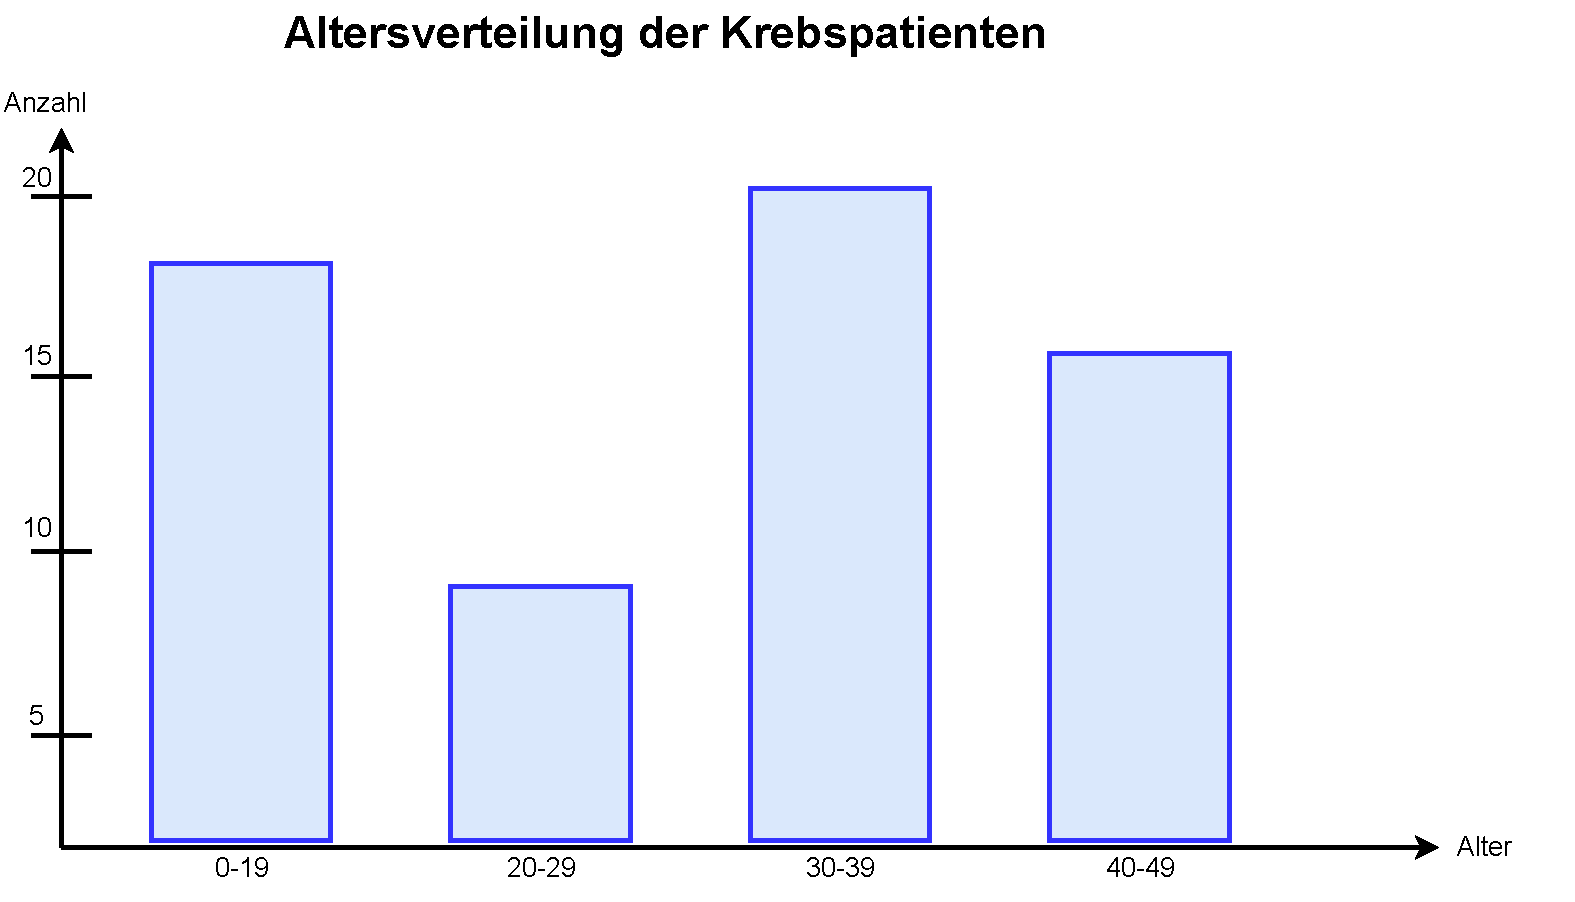
\includegraphics[scale=0.4]{./images/age_cancer_9.pdf}
	\caption{Die Anzahl der Krebspatienten am 12.12.21.}
	\label{fig:age_cancer_9}
\end{figure}
\begin{figure}[htbp]
	\centering
	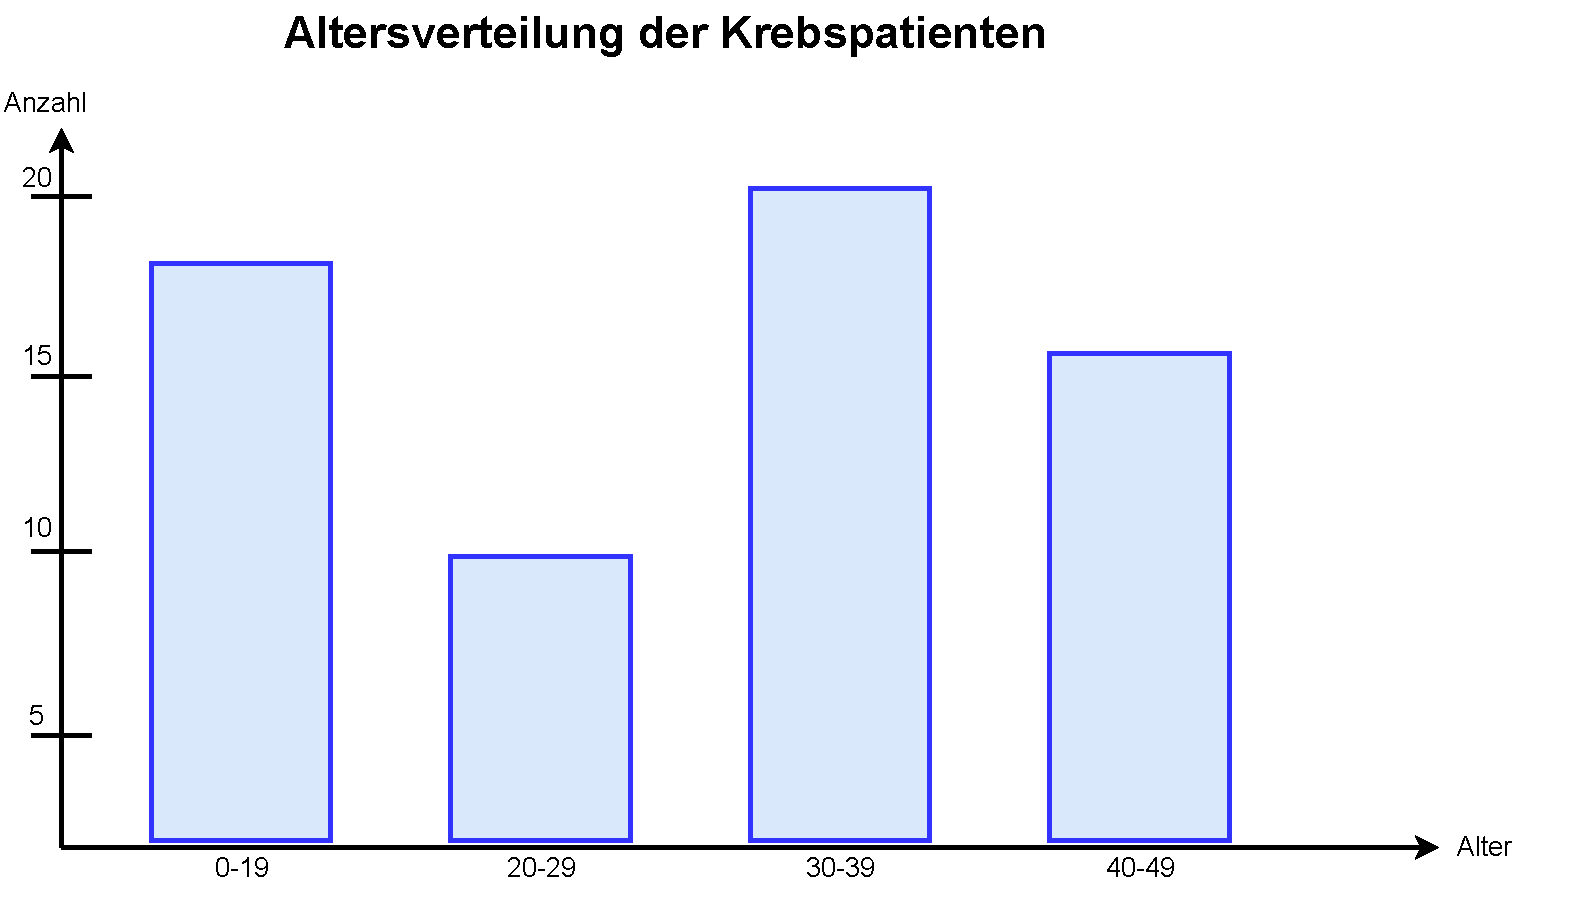
\includegraphics[scale=0.4]{./images/age_cancer_10.pdf}
	\caption{Die Anzahl der Krebspatienten am 13.12.21.}
	\label{fig:age_cancer_10}
\end{figure}

Ein Krankenhaus veröffentlicht täglich seine Statistik zu seiner Anzahl an krebskranken Patienten. Am 12.12.21 veröffentlicht es seine Statistik wie in \cref{fig:age_cancer_9} zu sehen ist. Sie gibt die Anzahl der Kranken nach ihrem Altersintervall an. So ist zum Beispiel die Anzahl der krebskranken Menschen im Alter von 20 bis 29 (inklusive) genau 9 Patienten. Diese Veröffentlichung ist nicht privatisiert und entspricht den tatsächlichen Werten. 

Wenn nun ein Freund Max wissen möchte, ob sein Bekannter Markus an Krebs leidet, dann muss er folgendes mindestens Wissen. Wie alt Markus ist und wann er in dieses Krankenhaus besucht hat. Wenn nun für Markus gilt, dass er 24 Jahre alt ist und am 13.12.21 im Krankenhaus war, dann folgt folgendes. Durch den Vergleich der Tabelle \cref{fig:age_cancer_9} und \cref{fig:age_cancer_10} im Altersintervall 20 bis 29 erfolgt aus der Differenz (10-9), dass eine zusätzliche Person erkrankt ist. Dies trifft dann auf Markus zu, sodass sein Freund Max nun weiß, dass Markus an Krebs erkrankt ist. Die Privatsphäre von Markus ist somit verletzt worden.

\textbf{Erweiterung von \gls{dp}: }
\gls{dp} kann um den additiven Parameter $\delta$ erweitert werden, sodass die Voraussetzungen, dass Informationen versehentlich durchsickern, bis zu einem gewissen Grad $\delta$ unerfüllt bleiben \parencite{Seminar2017}. Die Rückführung der Daten auf die originalen ist verhindert, wenn $\delta$ klein gewählt wird. Der Wert für $\delta$ hängt von der Größe der Datenbank ab. Diese Erweiterung heißt $(\epsilon,\delta)$- Differential Privacy und ist wie gefolgt definiert:
\begin{equation*}
	\Pr\Bigl[ \mA\Bigl( \mD_{1} \in \mS \Bigr) \Bigr]\leq  e^{\epsilon} \times \Pr\Bigl[ \mA\Bigl( \mD_{2} \in \mS \Bigr) \Bigr] + \delta
\end{equation*}
Ein randomisierter Mechanismus $\mA : \mD\longrightarrow\mathcal{S}$ mit der Eingabe eines Datensatzes sei gegeben, welcher alle potenziellen Ausgaben $S$ berechnet. Hierbei sind $\mD_{1}$ und  $\mD_{2}$ beliebige Datensätze, welche sich nur in einem Eintrag unterscheiden. Des Weiteren gilt für alle Untermengen $\mS \in \mathcal{S}$.

\subsection{Laplace Mechanismus}
Ein Mechanismus dient als randomisierter Algorithmus von \gls{dp}, um durch seine Funktion mathematisches Rauschen zu erzeugen. Dieses addierte Rauschen bewirkt das Abändern der Originalwerte im Rahmen der Vorgabe.

Der Laplace Mechanismus basiert auf der Laplace Verteilung wie in \cref{fig:fig_laplace_dib} veranschaulicht. Dieser Mechanismus berechnet das hinzugefügte Rauschen der Daten, um sie durch die Einhaltung von \gls{dp} zu privatisieren. Dafür spielt ebenfalls die Sensibilität \parencite{Seminar2017} der Daten eine Rolle, weswegen sie zuerst erklärt wird.

Sei $\mD$ ein Datensatz und $f: \mD \longrightarrow \mathbb{R}$ eine reellwertige Funktion. Die Sensibilität einer Funktion bezeichnet mit $\Delta f$ ist definiert als: 
\begin{equation*}
	\Delta f = \max |f(x) - f(y)|
\end{equation*}\parencite{AlgoFoundations2014}
wobei das Maximum von allen Paaren des Datensatzes $x$ und $y$ in $\mD$ genommen werden, welche sich nur in einem Eintrag unterscheiden.

Die Sensitivität einer Funktion $f$ gibt das Ausmaß an, wie sehr im schlimmsten Fall die Daten durch ein einzelnes Individuum verändert werden kann und damit die erforderliche eingeführte Veränderung der Antwort, um die Beteiligung einer einzelnen Person zu verbergen.
Durch die Sensitivität einer Funktion wird eine Obergrenze angesetzt, welche ein Maß angibt, wie stark die Ausgabe verrauscht werden muss, um die Privatsphäre zu bewahren.
\pgfmathdeclarefunction{laplace}{2}{%
	\pgfmathparse{1/(2*#2)*exp(-abs(x-#1))/#2)}%
}
\begin{figure}[htbp]\centering
	\begin{tikzpicture}
		\begin{axis}[every axis plot post/.append style={
				mark=none,domain=-3:3,samples=500,smooth,at={(0,0)},
				anchor=north east},
			axis x line*=bottom,
			axis y line*=middle, 
			enlargelimits=upper] 
			\legend{$\mu=0$ $b=1$,$\mu=0$ $ b=2$,$\mu=0$ $ b=4$}
			\addplot {laplace(0,1.0)};
			\addplot {laplace(0.0,2.0)};
			\addplot {laplace(0.0,4.0)};
		\end{axis}
	\end{tikzpicture}
	\caption{Die Laplace Verteilung um den Punkt ($0$,$0$) zentriert.}
	\label{fig:fig_laplace_dib}
\end{figure}

Auf Grundlage der Laplace-Verteilung wie in \cref{fig:fig_laplace_dib} veranschaulicht wird das Rauschen berechnet. Für ihre Dichtefunktion wird zum einen der Parameter $\mu$, welcher für die Lokalität gilt, und zum anderen $b$, welcher zur Skalierung dient, benötigt. Im Falle dieses Mechanismus ist der Parameter $b$ durch $\epsilon$ bestimmt und am Punkt $0$ für $\mu$ zentriert. Dies entspricht der symmetrischen Version der Exponentialverteilung. Eine Zufallsvariable $X$ ist Laplace verteilt, wenn gilt $X \sim Lap(b)$.

Der Laplace Mechanismus berechnet das zufällige Rauschen zu jedem Eintrag im Datensatz. Dazu wird den einzelnen Einträgen in der Antwort zu einer Anfrage $f$ Rauschen nach der Laplace-Verteilung hinzugefügt. Die Definition lautet:
\begin{equation*}
	\mM_{Lap} (x,f,\epsilon) = f(x) + Lap\Biggl(\mu = 0, b = Lap(\frac{\Delta f}{\epsilon})\Biggr)
\end{equation*}
wobei die $X_{i}$ Zufallsvariablen der Laplace-Verteilung $Lap(\frac{\Delta f}{\epsilon})$ sind.


\textbf{Beispiel Histogramm Anfragen: }
Bei solch einer Anfrage wird das Universum $\mathbb{N}^{|X|}$ in Zellen partitioniert \parencite{AlgoFoundations2014}. Die Anfrage fragt nach der Anzahl der Datenbankelementen, die in jeder der Zellen liegen. Aufgrund der disjunkten Zellen steigt bzw. verringert sich die Anzahl der Datenbankelementen nur um eins, wenn eines hinzugefügt oder gelöscht wird. Die Differenz dieser Zelle ist zu den anderen genau $1$, somit hat die Anfrage die Sensibilität von $\Delta f$ = $1$. Bei einer Anfrage kann hiermit zu allen wahren Werten der Zellen das Rauschen unabhängiger Ziehungen aus $Lap(\frac{1}{\epsilon})$ hinzugefügt werden.


\textbf{Beispiel der Funktionalität: }
Die Variable $k$ bezeichnet die Anzahl der Personen mit einer grünen Augenfarbe in der Datenbank \parencite{DPEasy2018}. Nun sei der wahre Wert $k$, welcher nicht veröffentlicht werden kann. Denn sonst kann ein Angreifer dies mit seinem Wissen abgleichen und herausfinden, ob $k-1$ (die Zielperson hat grüne Augen) oder $k$ (die Zielperson hat keine grüne Augen) gilt. Dafür muss er nur die Anzahl der Personen mit grünen Augen aus seinem Wissen mit den der Datenbank vergleichen. 

Für die Privatisierung der Zahl wird Rauschen hinzugefügt und nun wird $k$ = 1003 veröffentlicht. Dagegen ist für dieses Beispiel der wahre Wert $k$= 1001.
Aus der Sicht des Angreifers stellt sich die Frage, mit welcher Wahrscheinlichkeit die originale Zahl 1000 oder 1001 ist. Diese Werte werden mit ihrem zugrundeliegenden Verrauschen in \cref{fig:k_value} gezeigt. Die Hypothese besagt $k$ =1001 ist wahrscheinlicher, denn es ist zutreffend ein Rauschen von Distanz 2 (1003-1001) anstatt 3 (1003-1000) zu erzeugen. Die Abschätzung des Angreifers wird schwieriger desto kleiner $\epsilon$ ist.

\begin{figure}[htbp]
	\centering
	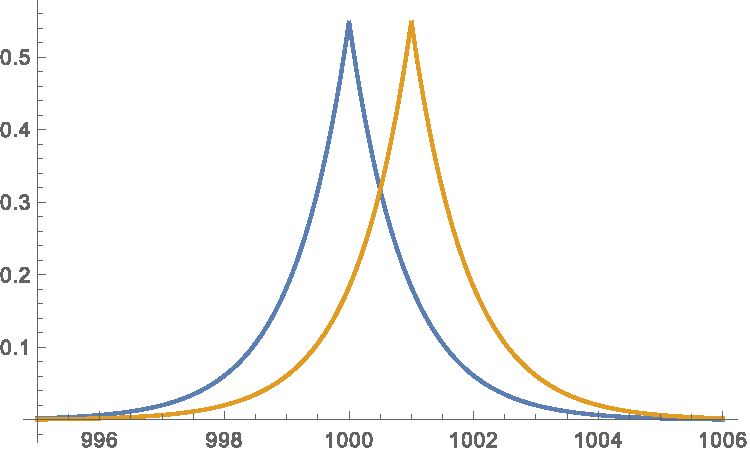
\includegraphics[scale=0.7]{./images/k_laplace_small_eps.pdf}
	\caption{Der wahre Wert ist k=1000 (die blaue Linie) oder k=1001 (die gelbe Linie) \parencite{DPEasy2018}}
	\label{fig:k_value}
\end{figure}

Somit wird dem Angreifer die Zuordnung eines Wertes durch die Überlappung der verschiedenen Laplace Verteilungen erschwert. Bei einem kleineren $\epsilon$ Wert folgt eine größere Abflachung der Verteilungen. 


\subsection{Gauß Mechanismus}
Analog zum Laplace Mechanismus, berechnet der Gauß Mechanismus das Rauschen basierend auf der Gauß Verteilung \parencite{AlgoFoundations2014}. Die Varianz ist von den Parametern für die Privatisierung und der Sensibilität abhängig.

Für beliebige Werte von $\delta \in (0,1)$ und $\epsilon \in (0,1)$ ist der Gauß Mechanismus wie folgt definiert:
\begin{equation*}
	\mM_{Gauss} (x,f,\epsilon,\delta) = f(x) + \mathcal{N}\Biggl(\mu = 0, \sigma^2 = \frac{2\ln(\frac{1.25}{\delta}) (\Delta f)^2}{\epsilon^2} \Biggr)
\end{equation*}

Die Besonderheit bei diesem Mechanismus liegt darin, dass er $(\epsilon,\delta)$-\gls{dp} garantiert, falls $\epsilon < 1$  erfüllt ist. Des Weiteren ist für diesen Mechanismus der Parameter $\delta$ notwendig.

\subsection{Weiterer Mechanismus}
Ein weiterer Mechanismus ist der \gls{rr}, welcher Rückschlüsse auf einzelne Personen verhindern soll \parencite{Seminar2017}. Dies wird hauptsächlich in sozialwissenschaftlichen Studien genutzt, um den Teilnehmer die Möglichkeit zu bieten, brisante Fragen ehrlich beantworten zu können. Aufgrund der verschiedenen Varianten von Randomized Response wird hier die gängigste Variante erklärt, welche auf einem Münzwurf basiert

\begin{figure}[htbp]
	\centering
	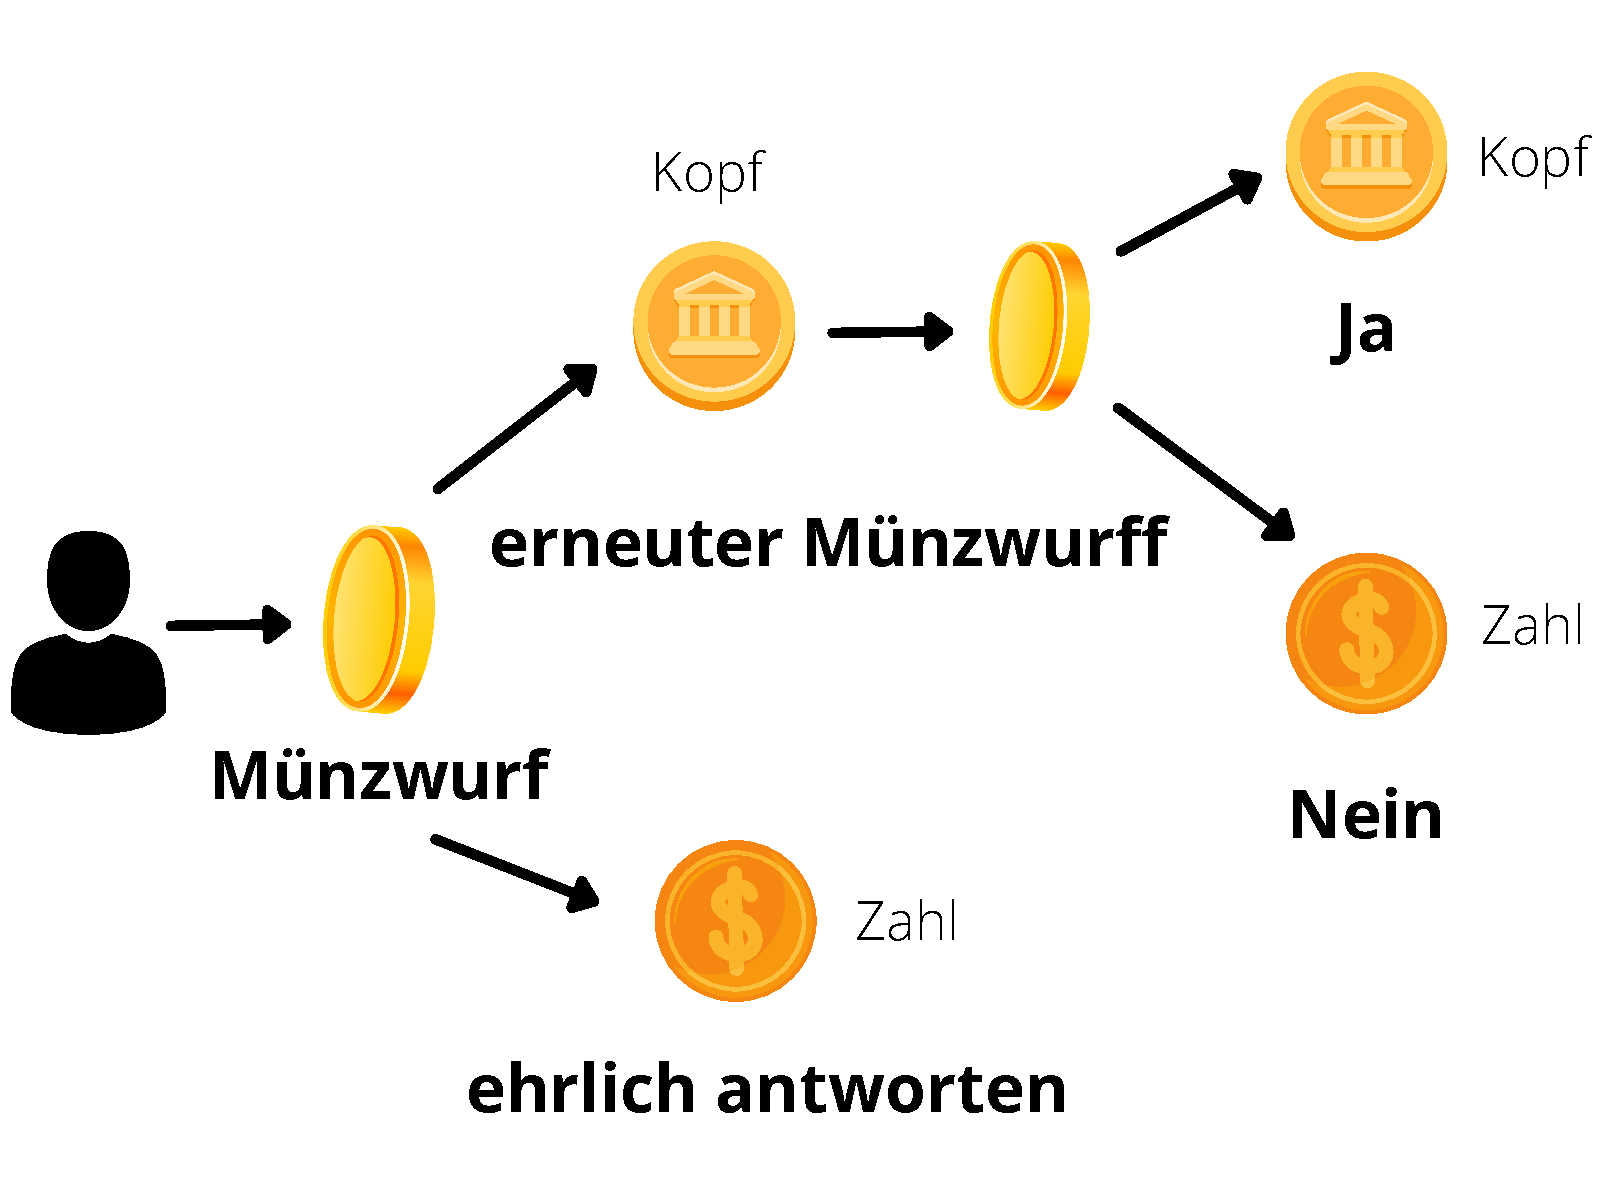
\includegraphics[scale=0.3]{./images/throw_coint.pdf}
	\caption{Eine Veranschaulichung der Entscheidung eines Befragten nach dem \gls{rr} Mechanismus.}
	\label{fig:rr_image}
\end{figure}

Der Befragte wirft eine Münze und folgt der Anweisung wie in Abbildung \cref{fig:rr_image} beschrieben. Wenn die Person beim ersten Wurf eine Zahl erhält, dann beantwortet sie die Frage ehrlich, sonst wirft sie die Münze noch einmal. Beim zweiten Wurf folgt bei Zahl die Beantwortung der Frage mit Nein, sonst mit Ja.

Die Intuition hinter diesem Mechanismus ist, dass dieser Abstreitbarkeit unterstützt. Wenn die Frage z.B. mit \enquote{Ja} beantwortet wurde, kann dies aufgrund des ersten und zweiten Wurfs, welche Kopf waren, geschehen sein. Die dazugehörige Wahrscheinlichkeit beträgt dann $\frac{1}{4}$. 
Es bleibt also ungewiss, ob die Person die Frage ehrlich beantwortet oder ob sie die Antwort der Münze wiedergibt. 
Dieser Prozess lässt eine Interpretation der Antworten zu, da die Art und Weise wie die Antworten eingeholt werden, nicht eindeutig nachvollziehbar sind.

Bei solchen Zufallsexperimenten wie dem Münzwurf nähert sich das Ergebnis bei häufiger Wiederholung dem erwarteten. Somit kann man davon ausgehen, dass die Hälfte der Antworten ehrlich angegeben worden sind. Dieser Mechanismus erfüllt \gls{dp}, genauer $\epsilon = ln(3)$.

\subsection{Privatsphäre-Metriken}
Im Bereich der Privatsphäre dienen die Metriken DP-res und Wasserstein Distanz als Messwert, inwieweit die Definition von \gls{dp} eingehalten wird und wie gut die Qualität des Verrauschens ist. Zum einen prüft die Metrik DP-res die Einhaltung von \gls{dp} nach und zum anderen die Metrik Wasserstein Distanz misst die Verschiedenheit der Datensätze nach dem Verrauschen.

\paragraph{DP-res (($\epsilon$,$\delta$)-DP begrenztes Histogramm Test)}
Dies ist ein $(\epsilon, \delta)$ \gls{dp} Histogramm Test aus dem Framework smart-noise-eval (siehe Kapitel 2.2) für benachbarte Datensätze D1 und D2. Das Ergebnis ist entweder wahr oder falsch.
Hierfür werden die beiden Datensätze durch die Ausführung einer Funktion (z.B. Durchschnittsfunktion) in angegebener Häufigkeit berechnet. Aus den aggregierten Daten wird zunächst ein Histogramm erzeugt. Anschließend folgt der Test der Histogramme, ob sie \gls{dp} einhalten. In diesem Test werden die Werte des Histogramms des erste Datensatzes mit $e^\epsilon$ multipliziert und mit $\delta$ summiert, wobei überprüft wird, ob das Histogramm in den Grenzen des zweiten Datensatzes liegt. Ebenfalls erfolgt dies umgekehrt.

\textbf{Interpretation für \gls{dp}: }
Das Ergebnis des Testes sagt aus, inwieweit die Definition von \gls{dp} eingehalten wurde. Wenn das Ergebnis wahr ist, dann ist es gültig, sonst nicht.
\paragraph{Wasserstein-Distanz}
Die Wasserstein-Distanz \parencite{WDExplanation} ist ein Maß um die Distanz zwischen zwei Wahrscheinlichkeitsverteilungen zu berechnen. Sie wird auch als \enquote{Earth Mover's distance} in der Dimension 1 bezeichnet. Dieser Name folgt aus der Interpretation von ihr als das Minimum der Energiekosten für das Verschieben und Transformieren eines Erdhaufens in Form einer Wahrscheinlichkeitsverteilung in die Form der anderen Verteilung. Für diese Bachelorarbeit wird die erste Dimension der Distanz benötigt, sodass sie als numerische Metrik genutzt werden kann. In der \cref{fig:wd} wird diese Interpretation veranschaulicht. Die kleinen blauen und roten markierten Stellen des Graphen sollen ineinander überführt werden. Dafür wird zum einen durch den Pfeil die Distanz gekennzeichnet und zum anderen die Wahrscheinlichkeit für die Umformung beachtet.


Die Distanz zwischen zwei diskreten Distributionen $f$ und $g$ ist wie folgt definiert:
\begin{equation*}
	\mW_{1} (f,g) = \inf_{h \in \mH(\mX,\mY|f,g)} \mE_{(x,y)\sim h} \Bigl[|\mX - \mY|\Bigr]
\end{equation*}
Hierbei ist $\mH$ eine Menge von allen vereinten Verteilungen der Variablen $\mX$ und $\mY$, welche die marginale Verteilungen $f$ und $g$ haben.
\begin{figure}[htbp]
	\centering
	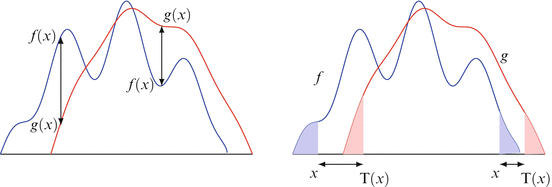
\includegraphics[scale=0.4]{./images/wasserstein_distance.png}
	\caption{Der Transport von $x$ nach $\mT(x)$ und andersherum wird mit der $\mW_{1}$ im rechten Bild berechnet, wobei die Flächen von f und g gleichgesetzt werden. \parencite{Santambrogio2015}}
	\label{fig:wd}
\end{figure}

Eine intuitive Interpretation dieser Metrik ist die Summe der Flächen zwischen zwei kumulativen Dichtefunktionen. Wenn $\mF(x)$ und $\mG(x)$ die kumulativen Dichtefunktionen von $f(x)$ und $g(x)$ sind, dann kann $\mW_{1}$ auch definiert werden als:

\begin{equation*}
	\mW_{1} (f,g) = \int_{\infty}^{\infty} |\mF(x) - \mG(x)| dx
\end{equation*}
\parencite{WDDef}
Die Wasserstein-Metrik ist eine echte Wahrscheinlichkeitsmetrik und berücksichtigt sowohl die Wahrscheinlichkeit als auch den Abstand zwischen verschiedenen Ergebnisereignissen.

\textbf{Interpretation für \gls{dp}: }
Diese Metrik kann sehr gut für die numerische Ähnlichkeit der originalen und verrauschten Daten eingesetzt werden. Des Weiteren kann der Wert der Metrik in Bezug für verschiedene $\epsilon$- Werte zur Veranschaulichung der Hinzunahme von Rauschen verwendet werden. Somit kann die Qualität der Frameworks in der Berechnung des Rauschens verglichen und ausgewertet werden.

\subsection{Genauigkeits-Metriken}
Im Bereich der Genauigkeit diene die Metriken die mittlere quadratische Abweichung und Standardabweichung als Messwerte, inwieweit das Verrauschen auf die Qualität der Genauigkeit einen Einfluss hat. Bei niedrigen $\epsilon$ Werten ist eine große Ungenauigkeit zu erwarten, bei großen soll das Gegenteil zutreffen.
\paragraph{Mittlere quadratische Abweichung}
Die mittlere quadratische Abweichung (in Englisch \gls{mse}) \parencite{MSE2022} gibt an, wie sehr ein Punktschätzer um den zu schätzenden Wert streut.
Wenn eine geringe mittlere quadratische Abweichung gilt, dann folgt gleichzeitig ein kleiner Bias und eine kleine Varianz des Schätzers. Der Schätzer liegt somit im Mittel in der Nähe des zu schätzenden Funktionals (kleiner Bias) und die Schätzwerte streuen wenig (kleine Varianz). Die Wahrscheinlichkeit, dass Schätzwerte in der Nähe ihres Erwartungswertes liegen, ist somit groß.

Ihre Definition lautet:

Sei $\mathcal{Y}$ der Vektor der beobachteten Werte und $\grave{\mathcal{Y}}$ der Vektor der vorhergesagten Werte. Der Vektor von $n$ Vorhersagen wird durch eine Stichprobe mit $n$ Datenpunkten aller Variablen und der vorherigen Vektoren generiert. Innerhalb der Stichprobe wird die mittlere quadratische Abweichung wie folgt berechnet:
\begin{equation*}
	MSE = \frac{1}{n} \sum_{i=1}^{n} (\mathcal{Y}_{i} -\grave{\mathcal{Y}}_{i})^2
\end{equation*}

\textbf{Interpretation für \gls{dp}: }
In Kontext von \gls{dp} kann anhand der mittleren quadratischen Abweichung die Genauigkeit der verrauschten Daten berechnet werden. Dafür gelten die originalen Daten der Funktion (z.B. der Durchschnitt) der tatsächlichen Stichprobe und die vorhergesagten Datenwerten der verrauschten Daten. Wenn das berechnete Resultat nahe an $0$ ist, gilt für die verrauschten Daten eine hohe Genauigkeit.

\paragraph{Standardabweichung}
Wenn die Quadratwurzel der Varianz genommen wird, dann ist der entsprechende Wert die Standardabweichung \parencite{SDLexikon} , welche als eines der wichtigsten Streuungsmaße in der Stochastik gilt.
Die Varianz ist definiert als die zu erwartende quadratische Abweichung einer Zufallsvariable zu ihrem Erwartungswert. Dagegen ist die Standardabweichung die durchschnittliche Entfernung aller gemessenen Daten vom Durchschnitt.

Wenn die Standardabweichung \parencite{SDNormalverteilung} der Daten berechnet wird, liefert sie die Information, wie weit sich diese Daten zwischen dem Minimum und dem Maximum verteilen, vor allem wie dicht sie sich um den Mittelwert häufen. Die Verteilung der Datenpunkte kann in einer Kurve dargestellt werden, welche meistens die Form einer Glocke hat. Dies wird in \cref{fig:nv_std} deutlich. Die Werte liegen entsprechend der Normalverteilung vor und die Standardabweichung zeigt die räumliche Distanz zum Mittelwert.

Sei $\mX$ eine Zufallsvariable und ihr Erwartungswert $\mathbb{E}(X)=\mu$, dann ist die Standardabweichung \parencite{Varianz}:
\begin{equation*}
	SD(\mX) := +\sqrt{VAR(\mX)} = +\mathbb{E}((\mX-\mu)^2)
\end{equation*}
Auch als $\sigma_{x}$ bezeichnet.

\begin{figure}[htbp]
	\centering
	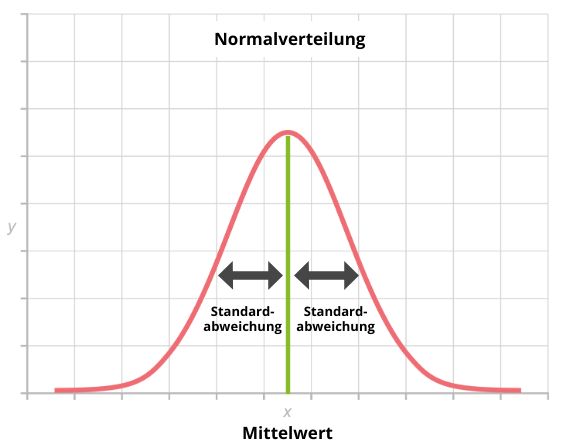
\includegraphics[scale=0.7]{./images/standard_deviation.png}
	\caption{Die Funktionalität der Standardabweichung. \parencite{STD}}
	\label{fig:nv_std}
\end{figure}

\textbf{Interpretation für \gls{dp}: }
In Kontext von \gls{dp} kann anhand der Standardabweichung bestimmt werden, inwiefern die Ausgabe durch das Rauschen des Laplace Mechanismus streut. Wenn die Standardabweichung klein ist, dann unterscheiden sich die verrauschten Ausgaben nicht sehr voneinander. Andersherum gilt dies auch. Dies gilt für den Laplace Mechanismus.

Insbesondere beim Gauß Mechanismus mit seiner Gauß-Verteilung kann eine Normalverteilung vorliegen, sodass sie sich zur Quantifizierung von Unsicherheit bei Entscheidungen unter Risiko eignen kann. In gewissen Intervallen der Standardabweichung ($\pm\sigma_{x}$, $\pm2\sigma_{x}$ usw.) kann die Wahrscheinlichkeit für das Aufkommen der Werte in einem Intervall berechnet werden. Dies kann zur Bewertung des Verrauschens benutzt werden.

\subsection{Erwartungstreue-Metrik}
Im Bereich der Erwartungstreue dient die Metrik mittlere vorzeichenbehaftete Abweichung als Messwert, inwieweit das Verrauschen die Werte verzerrt hat. Desto mehr die Werte verzerrt sind, desto weniger sind sie semantisch nutzbar. Die Aussagekraft der verrauschten Werte gegenüber den originalen verschwindet dadurch.
\paragraph{Mittlere Vorzeichenbehaftete Abweichung}
Die mittlere vorzeichenbehaftete Abweichung wird im Englischen als \gls{msd} bezeichnet.
Es gibt eine Menge von $n$ Paaren ($\theta_{i}$,$\hat{\theta_{i}}$), wobei $\theta_{i}$ für den tatsächlichen Wert und $\hat{\theta_{i}}$ für den geschätzten Wert steht \parencite{MSD}. Die Definition lautet:

\begin{equation*}
	MSD(\hat{\theta_{i}}) := \frac{1}{n} \sum_{i=1}^{n}  \hat{\theta_{i}} - \theta_{i}
\end{equation*}

\textbf{Interpretation für \gls{dp}: }
Bei dieser Metrik wird die Differenz von dem originalen Wert und dem verrauschten Wert paarweise berechnet und davon dann insgesamt der Mittelwert genommen. Dieser Wert veranschaulicht, ob durchschnittlich das Rauschen des Mechanismus zu viel (positiver Wert) oder zu wenig (negativer Wert) war. Somit kann das Verhalten des Mechanismus aufgezeigt und Schlüsse gezogen werden, ob die Informationen in den Daten erhalten bleiben.
\newpage
\section{Technische Aspekte der Frameworks}
In diesem Abschnitt werden die drei Frameworks in ihrer gesamten Struktur erklärt. Dies beginnt mit dem Aufbau des Frameworks bis zu seinen Besonderheiten, die es von den anderen abgrenzt. Zum Schluss folgt eine allgemeine Übersicht des Frameworks für den Einsatz in \gls{dp}.
\subsection{Smartnoise SDK}
\textbf{Technologie: }
Dieses Framework \parencite{Smartnoise}  kann in der Programmiersprache Python genutzt werden. Des Weiteren werden für zusätzliche Funktionalitäten die SQL-Sprache benötigt, um über die bereitgestellten Funktionen hinaus agieren zu können.

\textbf{Aufbau: }
Dieses Framework wird in drei Module smartnoise-sql, smartnoise-synth und smartnoise-eval untergliedert. Jeder dieser Teilbestände ist eine eigene Bibliotheken. Für diese Arbeit ist lediglich smartnoise-sql relevant. In der Teilbibliothek smartnoise-sql werden durch SQL-Anfragen innerhalb der Programmiersprache Python Daten ausgelesen und ihr Ergebnis verrauscht. Die Funktionalität stammt ursprünglich aus der Bibliothek \gls{opendp} \parencite{OpenDP}. Sie ist eine Ansammlung an statistischen Algorithmen, die die Definition von \gls{dp} einhalten. Durch die Anfragen können diese Berechnungen daraus vollzogen werden. 

\textbf{Beschreibung der Funktionen: }
Durch fünf verschiedene Methoden können Daten im Framework eingelesen werden. Unter diesen ist eine Datenbankverbindung möglich. Für das Nachverfolgen des \gls{pb}s steht die Funktionalität \enquote{odometer}(Kilometerstand) zur Verfügung. Während der Auswertung kann die Menge an benötigtem \gls{pb} eingesehen werden. Durch weitere Funktionen der Lesemethode \enquote{readers} kann die durchschnittliche Genauigkeit der Anfragen innerhalb eines Intervalls; z.B. 95\% der Fälle angegeben werden. Für die Veranschaulichung der Daten wird beim Histogramm automatisch Angaben wie der Nachname gelöscht, die die Privatsphäre verletzen könnten.

\textbf{Besonderheit: }
Eine direkte Verbindung zu einer SQL-Datenbank ist durch dieses Framework möglich. Hierbei ist ein unmittelbarer Zugriff auf die Originaldaten nicht von Nöten.

\textbf{Fazit: }
Insgesamt deckt dieses Framework die grundlegenden Funktionen für eine Auswertung durch seine Funktionalitäten ab. Des Weiteren bietet es fünf verschieden Möglichkeiten, um Daten auslesen zu können.

\subsection{IBM DP}
\textbf{Technologie: }
Dieses Framework \parencite{diffprivlib} kann in der Programmiersprache Python genutzt werden. Neben den statistischen Funktionen stehen weitere Funktionen im Bereich des \gls{ml}s zur Verfügung.

\textbf{Aufbau: }
Dieses Framework kann in die vier großen Hauptkomponente Mechanismen, Modelle, Tools und Accountant des \gls{pb}s unterteilt werden. Die Mechanismen besitzen alle grundlegenden Funktionalitäten, welche \gls{dp} nutzen. 
Die Modelle sind für \gls{ml} mit \gls{dp} einsetzbar. Diese lassen sich in Clustering, Klassifizierung, Regression, Dimensionsreduktion und Vorverarbeitung untergliedern. Dagegen stellen die Tools generische Funktionen für \gls{dp} gerechte Datenanalyse an, worin ein verrauschtes Histogramm enthalten ist. Zuletzt kann \enquote{Accountant} zum Nachverfolgen des investierten \gls{pb} verwendet werden. Fortschrittliche Kompositionstechniken berechnen zusätzlich dabei den Verlust an Privatsphäre.

\textbf{Beschreibung der Funktionen: }
Die Funktionalität richtet sich eher nach \gls{ml} und bietet dementsprechend überwiegend solche Methoden an. Diese umfassen grundlegende wie z.B. logistische Regression, k\_means, pca usw. mit Verwendung von \gls{dp}.
Neben dessen können statistische Funktionen wie die Anzahl, Durchschnitt, Summe usw. durch vordefinierte Funktionen aufgerufen werden. Eine Besonderheit liegt darin, \gls{dp} gerechte Histogramme, auch multidimensionale, erzeugen zu können. Zusätzlich kann der Einsatz des \gls{pb}s durch Accountant nachverfolgt werden. Somit stehen dem Forscher die Funktionen in den Bereichen Mechanismen, Modelle, Tools und Accountant zur Einsetzung bereit.

\textbf{Besonderheit: }
Die Mechanismen umfassen auch Funktionen im Bereich des \gls{ml}s. Hierfür werden grundlegende Modelle mit einer verrauschten Ausgabe durch \gls{dp} angeboten.

\textbf{Fazit: }
Insgesamt liegt der Fokus dieses Frameworks eher im Bereich \gls{ml}. Darin sind Modelle vorhanden, die in den Eingaben sowie im Trainieren richtig benutzt werden müssen. Sonst können deren Ergebnisse nicht aussagekräftig sein. Daher richtet sich dieses Framework in diesem Bereich eher an Experten in \gls{ml}, die ihre Ideen umsetzten, möchten. Im Bereich \gls{dp} sind grundlegende Funktionen vorhanden und können für eine Datenanalyse genutzt werden.

\subsection{Google DP}
\textbf{Technologie: }
Dieses Framework \parencite{DPGoogle} kann in der Programmiersprache Java, C++ und Go genutzt werden. Dafür stehen drei verschiedene Block-Bibliotheken, die in den jeweiligen Sprachen die grundlegenden Funktionen für \gls{dp} gerechte Auswertung implementieren, zur Verfügung.

\textbf{Aufbau: }
Die gesamte Bibliothek Google \gls{dp} ist in Tools unterteilt, die verschiedene Anwendungen umfassen.
Für eine einfache Anwendung durch Nicht-Experten kann \enquote{Privacy on Beam} genutzt werden. Dies ist ein End-zu-End \gls{dp} Framework, welches auf Apache Beam gebaut ist. Dafür wird keine Vorkenntnis in \gls{dp} vorausgesetzt. Lediglich die Angabe des \gls{pb}s genügt als Parametrisierung für die Berechnung. Für diese Arbeit ist der \enquote{Stochastische Tester} irrelevant. Wie bei den anderen Bibliotheken ist es möglich, das eingesetzte \gls{pb} nachzuverfolgen. Für eine Anwendung mit der SQL-Sprache bietet dieses Framework die Schnittelle \enquote{ZetaSQL} an. Sie verfügt die Eingabe von Anfragen durch SQL und und stellt dafür eine Kommandozeilen-Schnittstelle bereit.

\textbf{Beschreibung der Funktionen: }
Durch die fertig implementierten Block-Bibliotheken werden jeweils 14 Funktionen von statistischen, wie z.B. der Durchschnitt, bis zu graphisch basierenden Funktionen, wie z.B. \enquote{Laplace thresholding}, bereit gestellt. Darüber hinaus können durch SQL-Anfragen Daten ausgewertet werden.

\textbf{Besonderheit: }
Eine flexible Anwendung dieses Frameworks ist durch die drei verschiedenen Programmiersprachen möglich. Für einen Einstieg in \gls{dp} ist Privacy on Beam geeignet.

\textbf{Fazit: }
Insgesamt liegt der Fokus dieses Frameworks einheitlich auf \gls{dp}. Es stehen verschiedene Anwendungen durch statistische Funktionen zur Verfügung, die in ihrer Funktionalität eingeschränkt sind. Eine übliche Auswertung durch SQL-Anfragen ist ebenfalls möglich.

\newpage
\section{Vergleich}
Eine Gegenüberstellung der Frameworks in verschiedenen Gebieten erfolgt in \cref{tab : compare_frameworks}. Die drei Frameworks stellen grundlegende statistische Methoden für eine Auswertung bereit. Die verwendeten Mechanismen fürs Verrauschen basieren auf den zwei grundsätzlichen und IBM \gls{dp} bietet zusätzlich noch den exponentiellen an.  Zwei der Frameworks sind einzig auf \gls{dp} fokussiert, IBM \gls{dp} umfasst ebenfalls das Thema \gls{ml}. Ein Gebrauch der SQL-Sprache ist außer beim IBM \gls{dp} möglich. Einzig Smartnoise SDK bietet eine Auslesung der Daten aus einer Datenbank an. Bei den restlichen ist dies nur durch Auslesen von CSV Dateien realisierbar. Eine Vielfalt an Programmiersprachen bietet das Google \gls{dp} an, und zwar drei verschiedene. Die anderen beiden können nur in Python eingesetzt werden. Als einziges Framework kann das Google \gls{dp} bei der Eingabe eines Algorithmus validieren, ob er nicht \gls{dp} einhält. Die Entscheidbarkeit des Überprüfers hierbei ist semi-entscheidbar.

\begin{table}[h]
	\centering
	\begin{tabular}{ l l l l} \toprule
		& \textbf{Smartnoise SDK} & \textbf{Google DP} & \textbf{IBM DP}  \\ \midrule
		\textit{bereitgestellte Funktionen}	&  & &\\ \hline
		Laplace Mechanismus	& X  & X & X\\
		Gaussian Mechanismus	& X & X & X\\
		Exponentieller Mechanismus	&  & & X\\
		Summe	&  X & X & X\\
		Varianz   &  X & X & X\\
		Standardabweichung & X & X &X\\
		Anzahl	&  X & X & X\\ \hline
		\textit{Besonderheiten} & & &\\ \hline
		Modelle (\gls{ml})	&  & & X\\ 
		SQL-Anfragen	&  X & X &\\ 
		Auslesungsart der Daten	&  SQL-Sprache&CSV  & CSV\\ 
		Programmiersprache	&  Python& Go, Jave \& C++ & Python\\ 
		DP Algorithmus Validierer	&  & X &\\ \bottomrule
	\end{tabular}
	\caption{Vergleich der Frameworks in ihren Eigenschaften.}
	\label{tab : compare_frameworks}
\end{table}


\chapter{Verwandte Arbeiten}
Die Privatisierung von Daten durch \gls{dp} wird nicht nur in der Medizin seit einigen Jahren verwendet, sondern auch in der Industrie wie z.B. von Apple für die Auswertung von Nutzern bei der Versendung von Emojis \parencite{Apple}. Diese Arbeit beschränkt sich auf das Gesundheitswesen und die Evaluationsmöglichkeiten von \gls{dp}.


Im Jahr 2014 forschten gemeinsam nach einem Ansatz Wissenschaftler Raquel Hill, Michael Hansen, Erick Janssen und weitere aus verschiedenen Universitäten \parencite{Hill2014} nach einem Ansatz für die Nutzbarkeit von \gls{dp} für wissenschaftlichen Daten. Der Datensatz über ungeschützten Geschlechtsverkehr und ungeplante Schwangerschaften von der Kinsey Institut bereitgestellt. Diese Daten wurden durch \gls{dp} mit verschiedenen Algorithmen wie zellen-basiert, kd-Baum-Partitionierung, Privolet-Algorithmus (ad-hoc) und Walvet (basic) generiert. Die Metriken der Evaluation dieser verrauschten Daten in der Nutzbarkeit unterteilten sich in zwei Kategorien: multivariate logistische Regression und die Wichtigkeit der Merkmale der Daten (z.B. Dimension). 
Zusätzlich werden vier verschiedene Methoden k-d Baum, Basis und adhoc (Privelet Algorithmus) für \gls{dp} angewandt, um das Rauschen für die Zellen und die Histogramme zu erzeugen.
Für die Evaluation wurde der Datensatz in zwei Teilmengen unterteilt. Alle drei Daten, der gesamte Datensatz (MART\_FINAL) und die zwei Teilmengen (MART\_RS1, MART\_RS2), wurden durch \gls{dp} mit den verschiedenen Methoden ausgeführt und das Chancenverhältnis (in Englisch odds ratio) aus der logistischen Regression verglichen. Schlussendlich wurde festgestellt, dass \gls{dp} hat mit dem großen Unterschied zwischen der Anzahl von Zeilen und der gedeckten Zellen durch die Abfrage in der Dimension (zweite Kategorie) sehr große Schwierigkeiten hat. Dabei der gesamte Datensatz bei der Evaluation stets schlechter ab. 

In dieser Bachelorarbeit wird zur Kompatibilität der Frameworks die Nutzung eines großen Datensatzes anstatt mehrere. Es findet keine Unterteilung des Datensatzes statt.

Ein interessanter Einsatz von \gls{dp} ist die Privatisierung von Texten \parencite{TEM2021}. Hier wird der Algorithmus \enquote{\gls{tem}} entwickelt, welcher eine höhere Nutzbarkeit als der state-of-art (Stand 2021) haben. Der Algorithmus ermöglicht für eine beliebige Distanzmetrik das Privatisieren von Wörtern. Die Besonderheit liegt in der spezifischen Ausführung des \enquote{Exponential mechanism}, welcher für den Entwurf eines \gls{dp} Algorithmus genutzt wird. Der Schritt zur Privatisierung wird zu einem Auswahlproblem verlegt. Das Eingabewort wird durch eines mit einer höheren Ähnlichkeit zum Eingabewort aus der Worteinbettung ersetzt. Das Rauschen kann dadurch abhängig von der Dichte der Worteinbettung hinzugefügt werden. In ihren Experimenten mit einem vergleichbaren Algorithmus erreicht \gls{tem} eine deutliche höhere Genauigkeit und Privatisierung beim selben Privatisierungsparameter ($\epsilon$).


Dieses Paper befasst sich in Gegensatz zu dieser Bachelorarbeit mit dem Themengebiet Machine Learning in Gegensatz zu dieser Bachelorarbeit, jedoch wird folgendes für die Evaluation der Frameworks deutlich: Die Genauigkeit und der Privatisierungsgrad ist durch eine Metrik messbar, eine Verbesserung der Resultate ist durch den Mechanismus für \gls{dp} entscheidend und die Weise der Hinzufügung des Rauschens zu den Daten spielt eine wichtige Rolle. In den drei evaluierten Frameworks werden die bekannten Mechanismen wie Laplace und Gauss selbst implementiert und eingesetzt bzw. von einer Third Party verwendet. Des Weiteren ist die Zuteilung des Rauschens bei ihnen unbekannt und kann eine erhebliche Auswirkung auf die Genauigkeit haben.


Des Weiteren gelang es den Wissenschaftlern der Pennsylvania State University in den USA wie ein \gls{dp} Framework, welches von Herrn Wasserman und Zhou entwickelt worden sind \parencite{DPFramework}, abgeändert werden muss, um für klinische Daten einsetzbar zu sein \parencite{Duy2009}. In solchen Anwendungsgebieten sind für Untersuchungen Hypothesen, welche üblicherweise statistisch getestet und modelliert werden, durch dieses Framework ermöglicht worden. Die Stichprobe ist entscheidend für die Effizienz und den Grad an Privatisierung der Daten. Beim Algorithmus von \gls{dp} wurde die Zerlegung in Gruppen für eine bessere Schätzfunktion durchgeführt und beim Laplace Mechanismus ein Parameter unterlassen, so dass bei einem festen Stichprobenumfang $N$ nur das $\epsilon$ anpasst werden muss, um das Verhältnis zwischen der Privatsphäre und den asymptotischen Eigenschaften des zurückgegebenen Schätzers zu bestimmen. Durch Experimente wurde gezeigt, dass dadurch der Mean Squared Error von \gls{dp} deutlich niedriger als die eines Maximum-Likelihood-Schätzers für dieselben Daten ist. Dies ermöglicht sensible medizinische Daten unter Einhaltung der Privatsphäre effizienter auszuwerten.


In dieser Bachelorarbeit wird ebenfalls die Einsetzbarkeit von \gls{dp} als Framework für medizinische Daten untersucht und evaluiert. Der Datensatz wird dagegen nicht unterteilt, sondern in der gleichen Größe für alle Frameworks bereitgestellt. Des Weiteren werden die Frameworks unverändert entsprechend der Definition von \gls{dp} eingesetzt. Diese Arbeit wird dem realistischen Einsatz von \gls{dp} für das Gesundheitswesen aus dem Paper nachgehen.

Unterstützt von der EURECOM sowie privaten Firmen entwickeln Eleonora Ciceri , Marco Mosconi, Melek Önen und Orhan Ermis die Plattform PAPAYA, um Datenschutzbedenken auszuräumen, wenn Datenanalyseaufgaben von nicht vertrauenswürdigen Datenverarbeitern durchgeführt werden. Dieses Projekt soll unter Einhaltung der DSGVO und des Schutzes der Kunden durchgeführt werden, während wertvolle und aussagekräftige Informationen aus den analysierten Daten extrahiert werden. Das PAPAYA-Projekt fokussiert sich auf drei Hauptdatenanalysetechniken: neuronale Netze (Training und Klassifizierung), Clusterbildung und grundlegende Statistiken (Zählung). PAPAYA widmet sich zwei Anwendungsfällen im Bereich der digitalen Gesundheit. Im ersten Bereich für Erkennung von Arrhythmie und Stress. Im zweiten Fall wird \gls{dp} für das Zusammenführen der personenbezogenen medizinischen Daten Angestellter für das neuronale Netzwerk eingesetzt. Einzelne Angestellte sind somit vor einer Veröffentlichung ihrer Daten bewahrt und das Netzwerk kann trotz dessen Berechnungen durchführen.


Dieser zweite Anwendungsfall entspricht dem dieser Bachelorarbeit in der Konstruktion. Den Patienten wird ermöglicht durch ihre \gls{ePa} ihre Daten der Forschung bereitzustellen, welche durch eine Datenbank zusammengeführt und anschließend durch \gls{dp} zur privatisierten Auswertung vorhanden sind. Die Frameworks basieren weder auf Machine Learning noch beinhalten solche Funktionen im Themenbereich der Klassifizierung. Sie bieten generelle statistische Funktionen für \gls{dp} Brechungen an. Des Weiteren gilt ebenfalls die Einhaltung der DSGVO für die Frameworks für den medizinischen Anwendungsfall.


Eine große und ausführliche Übersicht über die bisherigen Ergebnisse der Forschung bezüglich \gls{dp} bildet das Paper \parencite{OverviewDP} der CHEO Research Instituts. In diesem wird über die Begrenzungen des Verfahrens sowie seine Mechanismen (Laplace, Gauß usw.) gesprochen, die durch die Forschung zum Vorschein kam. Unter anderem sind Schwierigkeiten mit den Anfragen an Datenbanken aufgekommen, da die Genauigkeit mit vielen verschiedenen Anfragen abnimmt. Sonst kann ein Angreifer durch die verrauschten Ausgaben eine Fraktion einer Datenbank rekonstruieren. Des Weiteren folgt, dass das Rauschen aus dem Mechanismus linear mit der Anzahl der Anfragen wächst. Dies impliziert, dass bei sublinearem Rauschen des Mechanismus nicht in der gleichen Menge Anfragen beantworten kann. Als Resultat wird festgestellt, der Laplace Mechanismus garantiert die Beantwortung zufälliger Anfragen, ist effizient, erreicht $\epsilon$-\gls{dp} und beantwortet Anfragen anpassungsfähig. Jedoch erfüllt er das Kriterium, eine große Anzahl an Anfragen mit einer nicht einfachen Genauigkeit zu beantworten, nicht. Für die Anwendung von \gls{dp} im Gesundheitswesen, sind gewisse Umstände sehr zu beachten. Bei Anfragen für die Anzahl der Patienten mit einer gewissen Eigenschaft, ist nur durch ein abgewandelter Exponentieller Mechanismus erfolgreich. Eine vorgegebene Menge an Budget für den Parameter $\epsilon$, ermöglicht den Nutzern davon eins auszusuchen. Der Nutzer kann somit sein Parameter gerichtet an seiner Anfrage auswählen.


Dieses Paper zeigt mögliche Schwierigkeiten bei der Evaluation dieser Bachelorarbeit. Es wird eine einfache Anfrage (Durchschnitt) durchgeführt und der Laplace Mechanismus verwendet. Es wird auch keine Menge an $\epsilon$- Budget genutzt. Es wird eine große Menge an Anfragen stattfinden (1000 mal). Die Anwendbarkeit des Verfahrens auf den medizinischen Fall kann entsprechend der Ergebnisse beschränkt genutzt werden.

Insgesamt fehlt in der medizinischen Forschung die Untersuchung von Frameworks für das Gesundheitswesen. Es gibt vereinzelt Versuche, vor allem für Machine Learning, jedoch fehlt es an einer Evaluation in den Aspekten von Genauigkeit und Privatisierung von \gls{dp} Frameworks für die Medizin.




\chapter{Anwendungsfall}
Im Rahmen dieser Arbeit wird die Verwendung von \gls{dp} Frameworks evaluiert und dazu eine prototypische Schnittstelle implementiert. Das folgende Kapitel führt einen konkreten Anwendungsfall für die drei Frameworks auf, wobei auf eine Anwendung in der medizinischen Forschung eingegangen wird. Anschließend wird der Ursprung der generierten Daten erläutert.
\section{Geplante Forschungsdatennutzung in der ePa}
Alle gesetzlich Versicherten können seit dem 1. Januar 2021 eine elektronische Patientenakte (\gls{ePa}) ihrer Krankenkassen erhalten \parencite{BGMePa}. In dieser werden medizinische Befunde, Informationen aus vorhergehenden Untersuchungen und Behandlungen über Praxis- und Krankenhausgrenzen hinweg umfangreich gespeichert. Der Patient kann durch verschiedene Endgeräte in einer dazugehörigen App seine medizinischen Unterlagen digitalisieren und in der \gls{ePa} abspeichern. Diese Daten liegen dann verschlüsselt darin vor. Die Daten werden nicht nur lokal verschlüsselt gespeichert, sondern auch innerhalb einer Telematikinfrastruktur, die zur schnellen Kommunikation zwischen den medizinischen Beteiligten dient.  Wenn ein Patient einem Arzt Zugriff auf seine \gls{ePa} gewähren möchte, dann muss er sie durch seine elektronische Gesundheitskarte und seine persönliche Identifikationsnummer freischalten. Zudem benötigt der Arzt seine Identifikationsnummer auf seinem Heilberufsausweis, welche als ein zweiter Schlüssel zum Lesen der \gls{ePa} dient. Alleinig der Patient kann inhaltliche sowie zeitliche Zugangsbeschränkungen seiner Daten festlegen. In der ersten Version ab 2021 konnte der Patient einer dritten Person lediglich kompletten oder gar keinen Zugriff gewähren. vollkommenen oder gar keinen Zugriff zuweisen. Ab der Änderung (zweite Version) im Jahr 2022 ist das Konfigurieren individueller Zugriffsberechtigungen pro Dokument möglich. So kann ein Zahnarzt nur einen Bruchteil der \gls{ePa} seines Patienten lesen, ein Hausarzt hingegen die gesamten Dokumente. Für 2023 ist eine dritte Version angekündigt, bei der eine persönliche digitale Identität hinterlegt wird, eine Datenfreigabe für Forschungszweck möglich ist und weitere Funktionalitäten hinzukommen werden.

Nach dem eingeführten Patientendatenschutzgesetz können die Patienten mit der dritten Version der \gls{ePa} ihre Daten der Forschung freigeben, was als Datenspende bezeichnet wird. So können verschiedene Verbände wie der Bundesverband der Deutschen Industrie e.V. (BDI), Bundesverband Medizintechnologie (BVMed) und weitere auf diese medizinischen Daten zugreifen, um z. B. ihre Versorgungsforschung gezielter zu führen. Die Daten der Datenspender werden nach dem Patientendatenschutzgesetz auf zentralen deutschen Servern gespeichert. Sie unterliegen den europäischen Datenschutzbestimmungen.

Dieses geplante Vorhaben wird in der \cref{fig:useCase} abgebildet. Im linken Bereich wird das zuvor beschriebene Szenario für die dritte Version im Jahr 2023 veranschaulicht.

\section{Erweitertes Szenario durch DP}
In dieser Arbeit wird der Einsatz von Frameworks mit \gls{dp} Funktionen am Beispiel einer Forschungsschnittstelle
evaluiert. Dafür wird der Anwendungsfall um das folgende Szenario erweitert.
\begin{figure}[!htbp]
	\centering
	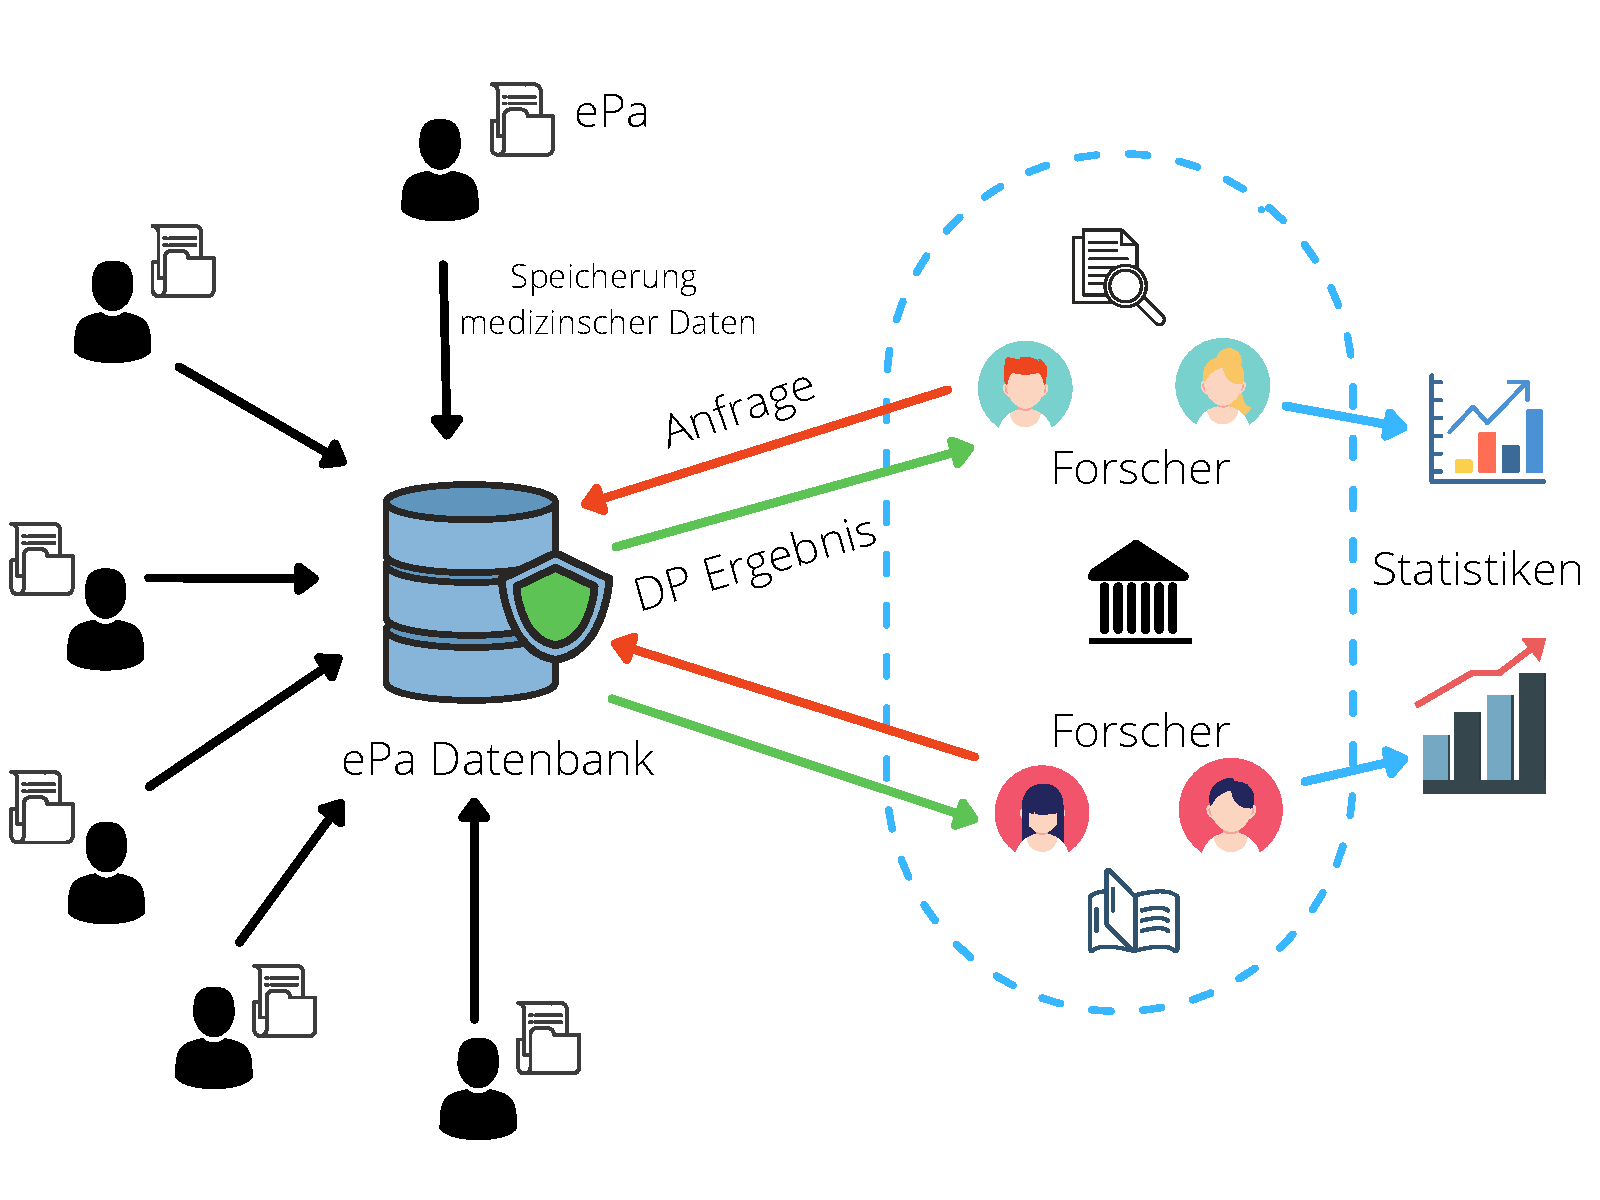
\includegraphics[scale=0.4]{./images/use_case.pdf}
	\caption{Die Visualisierung des Anwendungsfalls mit der Benutzung der \gls{ePa} und ihren dazugehörigen Akteuren.}
	\label{fig:useCase}
\end{figure}

Ein Forschungsinstitut stellt den Forschern ein Framework bereit, welches ein Zugriff unter der Bewahrung der Privatsphäre auf die \gls{ePa} Datenbank ermöglicht. In diesem Framework stellt ein Forscher eine Anfrage an die Datenbank. Das Framework verwertet die statistische Funktion der Anfrage unter Einhaltung von \gls{dp}, indem den Daten ein Rauschen hinzugefügt wird. Die hierfür benötigten Parameter des \gls{pb}s ist serverseitig festgelegt und nicht durch dritte Personen änderbar. Diese Parameter werden vom Staat in Einklang mit dem \gls{dsgvo} bestimmt und geändert (siehe Kapitel 1). Dieses verrauschte Ergebnis erhält der Forscher und verwendet es für seine Analysen und Statistiken. Anhand weiterer Anfragen können Zusammenhänge erkannt werden. Mit erfassten Kenntnisse können dann aussagekräftige Statistiken veröffentlicht werden. Hierbei wird nach der Definition von \gls{dp} die Beteiligung eines Patienten mit seiner \gls{ePa} nicht mehr ausschlaggebend, wodurch seine Privatsphäre geschützt wird.  

Dieses beschriebene Szenario dient als eine Weiterführung und wird in \cref{fig:useCase} im mittleren und rechten Bereich veranschaulicht.

\begin{figure}[htbp]
	\centering
	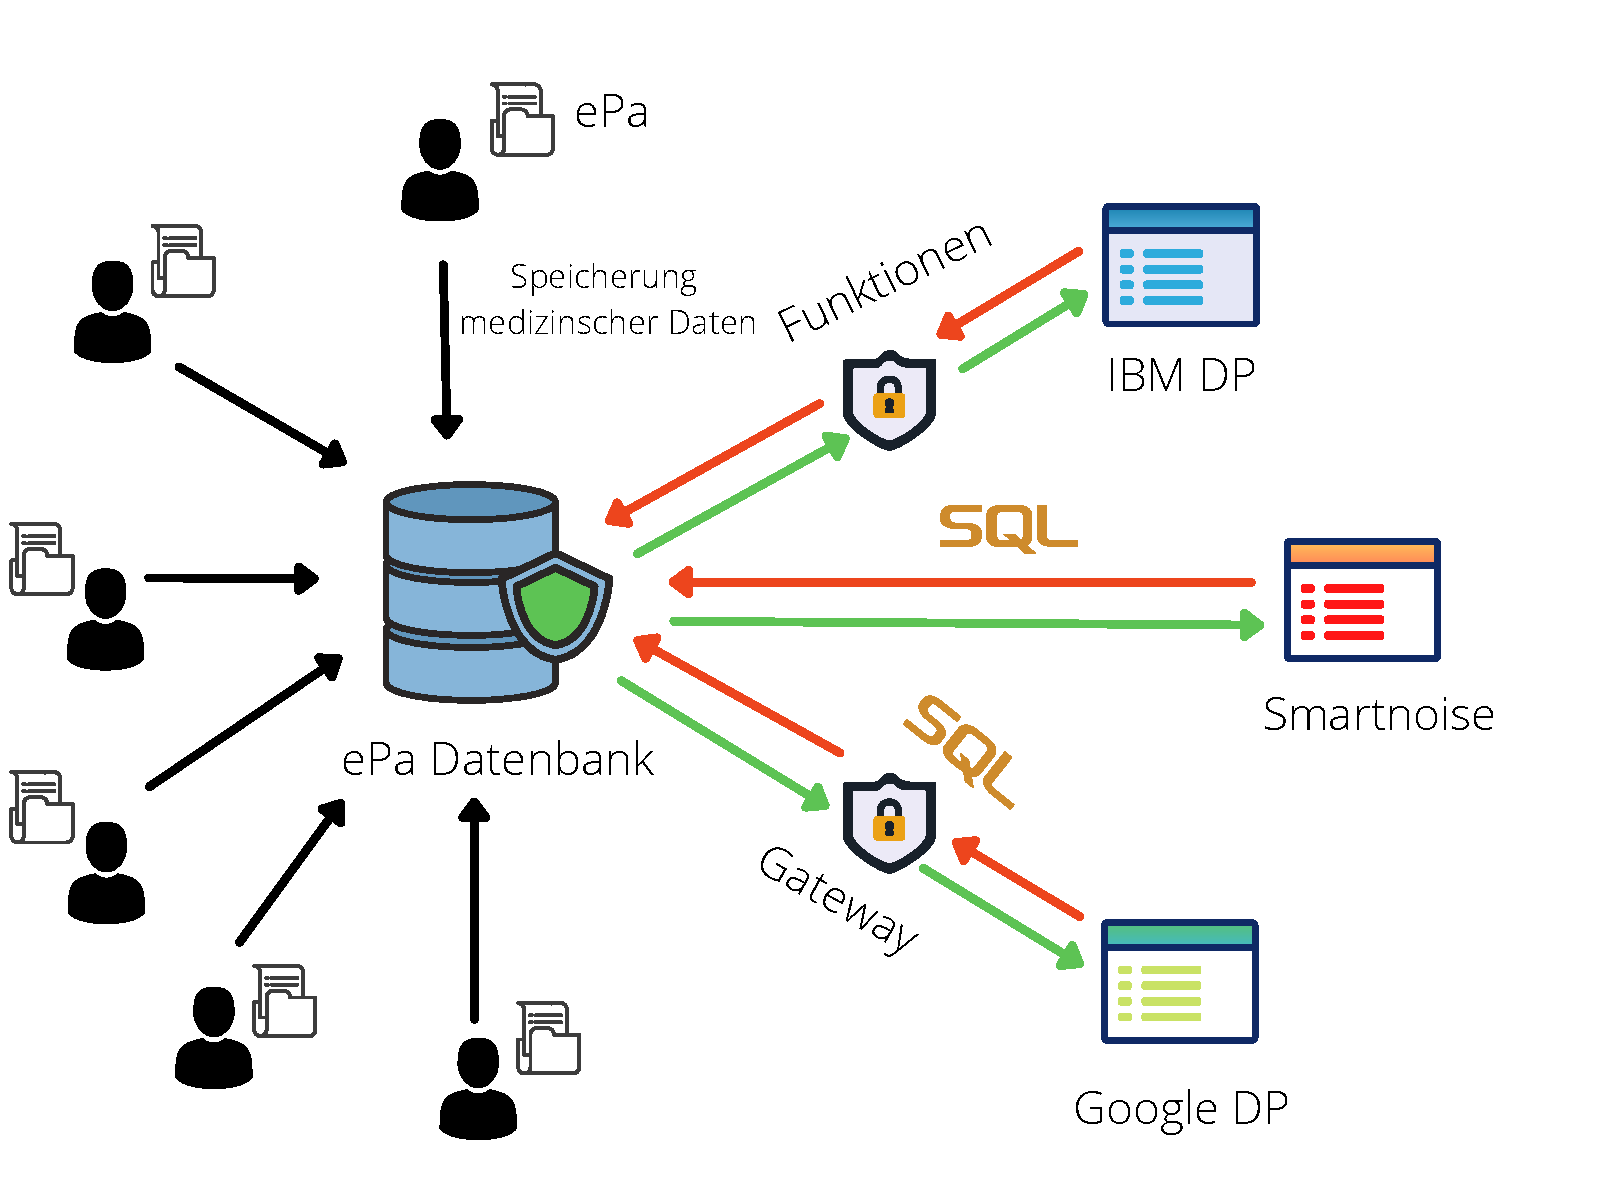
\includegraphics[scale=0.3]{./images/use_case2.pdf}
	\caption{Die Visualisierung des Anwendungsfalls mit der Benutzung der Frameworks.}
	\label{fig:use_case2}
\end{figure}

In Anbetracht des Szenarios kann eines der drei Frameworks eingesetzt werden. Der Einsatz eines jeweiligen Frameworks (IBM \gls{dp}, Smartnoise SDK und Google \gls{dp}) wird in der \cref{fig:use_case2} veranschaulicht. 
Das Smartnoise SDK Framework bietet zunächst die Verbindung zu einer Datenbank an. Aus dieser kann, ohne einen unmittelbaren Zugriff zu haben, Daten ausgelesen werden. Dagegen benötigen die Frameworks IBM \gls{dp} und Google \gls{dp} eine zusätzliche Verbindungsmöglichkeit zur Datenbank, denn sie können nur lokal Dateien auslesen. In den beiden Frameworks Smartnoise SDK und Google \gls{dp} werden die Anfragen durch die SQL-Sprache umgesetzt. Dabei werden die Parameter des \gls{pb}s durch den Forscher bestimmt, was dem Anwendungsfall widerspricht. Dies ist ebenfalls beim IBM \gls{dp} der Fall. Dieses Framework realisiert seine Anfragen anstatt durch die SQL-Sprache mit bereitgestellten statistischen Funktionen und \gls{ml} Modellen. Bei der Auswertung bietet dieses Framework noch zusätzlich die Generierung von verrauschten Histogrammen an. Dies kann in einer Statistik verwendet werden. Smartnoise SDK und Google \gls{dp} unterstützen explizit keine Funktionalitäten zur Visualisierung von Daten an, dagegen IBM \gls{dp} einige wenige wie z.B. verrauschte Histogramme.

\section{Rohdaten}
Für die Evaluation der Frameworks werden große Datenmengen benötigt. Diese sollen zu einem leicht verständlich sein und zugleich für den medizinischen Anwendungsfall geeignet sein. Dafür können synthetische Daten erzeugt oder bereits erfasste Daten im Gesundheitswesen genutzt werden. Für diese Bachelorarbeit wird ein hybrider Ansatz zwischen den beiden Möglichkeiten genommen. Zum einen wird eine CSV Datei vom \gls{rki} genutzt \parencite{RKIAltersverteilung}, welche die Anzahl an infizierten Patienten entsprechend der 19 Altersgruppen pro Kalenderwoche enthält. Für die Kalenderwochen 48 bis 52 (der Monat Dezember) wird die Wahrscheinlichkeitsverteilung der infizierten Personen pro Altersgruppe wie in \cref{tab : age_distribution} dargestellt, berechnet. Auf dieser Verteilung werden 1000 synthetisch generierte Werte für diese Altersgruppen erzeugt. Dieser Datensatz dient als Quelle für die Evaluation der Frameworks.

Zunächst wurde bei der Recherche ein großer Fokus auf Originaldaten im Bereich der Krankheit COVID-19 gesetzt. Verschiedene Institutionen und Länder haben Online-Portale sowie Datenbanken veröffentlicht, um die medizinischen Auswirkungen durch COVID-19 Krankheit in Zahlen auszudrücken

Dafür liegt ein großer Datenhub vom RKI vor, welcher die Covid-19 Infektionen pro 100.000 Einwohner der deutschen Bundesländern angibt \parencite{Datenhub}. Diese Statistik wird wöchentlich aktualisiert. Diese Datei mit tausenden Einträgen enthält genügend Informationen für die Evaluation und ist leicht durch eine CSV Datei einzulesen. Zusätzlich können die Anzahl der Attribute (Spalten) bestimmt werden. Jedoch sind die Daten zum einen inhaltlich teilweise schwierig zu verwenden, da sie schon privatisiert sind. Das Alter wird nur in Altersgruppen durch Kenneichungen angegeben und die Verteilung wird nach Bundesländern oder Landkreisen angeboten. Diese Problematik erschwert diese Datei als Basis der Evaluation zu verwenden.

Bei weiterer Recherche durch Kaggle, ein Online-Ansammlung von wissenschaftlichen Dokumenten, war eine Publikation des Landes Italien zur Krankheit COVID-19 sehr interessant \parencite{CovidItalien}. Hierbei handelt es sich um die Anzahl der Fälle sowie der Todesfälle nach Alter und Geschlecht für jede Region in Italien. Zwar ist die Datei an sich klein, jedoch können die darin enthaltenen Daten als Basis zur Synthese eines umfangreicheren Datensatzes genutzt werden. Das Ziel war für jedes Alter die spezifische Anzahl der Kranken zu erfassen. Aus Gründen der Privatsphäre wurden diese Daten schon privatisiert und nur in Altersgruppen veröffentlicht.
Nach weiterer Suche erfolgte der Fund desgleichen für Deutschland wie des von Italien, sodass dieser Datensatz für die Evaluation eingesetzt wird \parencite{RKIAltersverteilung}.
\begin{table}[ht]
	\centering
	\begin{tabular}{l l} \toprule
		\textbf{Altersgruppe} & \textbf{Wahrscheinlichkeit}  \\ \midrule
		0 - 4	&  4\% \\
		5 - 9	&  9\% \\
		10 - 14	&  10\% \\
		15 - 19	& 6\%  \\
		20 - 24	& 6\%  \\
		25 - 29	&  7\% \\
		30 - 34	&  8\% \\
		35 - 39	&  9\% \\
		40 - 44	&  8\% \\
		45 - 49	& 7\%  \\
		50 - 54	& 7\%  \\
		55 - 59	& 6\%  \\
		60 - 64	& 4.5\% \\
		65 - 69	&  3\% \\
		70 - 74	& 2\%  \\
		75 - 79	& 1\%  \\
		80 - 84	&  1,5\% \\
		85 - 89	& 0.5\%  \\
		90+& 0.5\%  \\ \bottomrule
	\end{tabular}
	\caption{Die Wahrscheinlichkeitsverteilung der COVID-19 infizierten Menschen nach den Altersgruppe im Dezember 2021.}
	\label{tab : age_distribution}
\end{table}


\chapter{Implementierung}
Der folgende Abschnitt umfasst die praktische Umsetzung dieser Bachelorarbeit. Zunächst werden grundlegende Tools für die Umsetzung der Schnittstelle dargestellt und ihre Anwendung erläutert. Anschließend folgt der Hauptteil dieser Arbeit, die generische Schnittstelle. In dieser werden die Daten für die Evaluation erzeugt und ausgewertet. Einige Probleme sind bei dieser Umsetzung aufgetreten, welche näher beleuchtet werden. Zuletzt werden selbst erstellte CSV Daten präsentiert, die für die generische Schnittstelle von Nöten sind.
\section{Benutzte Tools}
Als Programmierumgebung wurde Jupyter Notebook, eine web-basierte interaktive Umgebung, eingesetzt. Zwei der drei Frameworks (IBM \gls{dp} \& Smartnoise SDK) wurden in der Programmiersprache Python eingesetzt, wodurch in Jupyter Notebook ihre Funktionalität genutzt werden konnten. Nebenbei können durch weitere Python Bibliotheken einfach und schnell Grafiken für die Auswertung der Frameworks realisiert werden. Eine entscheidende Funktionalität dieser Umgebung ist die Unterstützung einer Verbindung zu Servern. Diese verhalf die zeitaufwendigen Berechnungen der Frameworks auf einen Server zu verlagern.

Dagegen wurde das dritte Framework Google \gls{dp} in der Programmiersprache Java umgesetzt, weshalb hierfür die Programmierumgebung Eclipse genutzt wurde. Die Erstellung des Projektes erfolgte durch Bazel, ein Build-Tool zur Automatisierung des Erstellens und Testens von Software. Durch Kommandozeilenbefehle wird der Code erzeugt und durch eine interne Datei von Bazel ausgeführt.

Für die aufwendigen und komplexen Berechnungen innerhalb der aufgerufenen Funktionen des Frameworks wurde ein Server mit den folgenden Systemspezifikationen genutzt: 

Plattform Linux-3.10 64 with-centos-7.9.2009-Core, 18 GB verfügbarer virtueller Arbeitsspeicher, 40 logische Prozessorkerne.

Über eine SSH Verbindung konnten die Berechnungen der Frameworks IBM \gls{dp} und Smartnoise SDK aus dem Jupyter Notebook auf dem Server ausgeführt werden. Dagegen wurde beim Google \gls{dp} das Programm lokal in der Programmierumgebung Eclipse ausgeführt. Zunächst bestand keine Notwendigkeit die Berechnungen auf den Server auszulagern, da die Evaluationsergebnisse schnell berechnet wurden.

\section{Generische Schnittstelle}
In der Datei \textit{source\_data.ipynb} werden die 1,000 generierten Alterswerte erzeugt. Darin wurde der in \cref{sourceData} dargestellte Algorithmus in Python implementiert. Zunächst wird die Verteilung der Wahrscheinlichkeiten für die 19 Altersgruppen in \textit{distribution} vorgegeben. Basierend darauf werden die Gewichte für die zufällige Auswahl des Alters innerhalb einer Altersgruppe festgelegt. Hierfür werden die Wahrscheinlichkeiten gleichermaßen für 100 Alterswerte \textit{weights} verteilt. Somit hat \textit{weights} eine Dimension von 1 Reihen und 100 Spalten. In der Schleife erfolgt 10-mal die Zuweisung von jeweils 100 Werten entsprechend der Gewichtung durch \textit{weights}. Letztendlich befinden sich dann 1000 synthetische Alterswerte in \textit{sourcedata} vor. Davon wird der originale Durchschnitt ohne Verrauschen 1000-mal genommen und in der Datei \textit{originalMean.csv} abgespeichert. Aus den 1000 Alterswerte werden zwei \textit{neighboring datasets} (benachbarte Datensätze) berechnet und in \textit{d1Data.csv} und \textit{d2Data.csv} gespeichert. Diese zwei Datensätze sind für die Berechnung der Metriken nach der Definition von \gls{dp} notwendig, die auf der Aussage von zwei Datensätzen basiert \parencite{Dwork2006}.
\begin{algorithm}[htbp]
	\caption{Erzeugung der 1000 Alterswerte basierend auf der Wahrscheinlichkeitsverteilung von Dezember}\label{sourceData}
	\begin{algorithmic}[1]
		\State $distribution \gets [4,9,10 ... 0.5,0.5]$
		\State $weights \gets [4,4,4,4,4,9,9,9,9,9,10 ... ,0.5,0.5,0.5,0.5,0.5]$
		\For{$i$ $to$ $10$}
		\State $sourceData\gets random.choices(range(0,100),
		weights, k=100)$	
		\EndFor
	\end{algorithmic}
\end{algorithm}

In der Datei \textit{metrics.ipynp} ist das Objekt \textit{Metrics} mit seinen Attributen definiert. Diese sind die Metriken der Evaluation. Ab dem Kaptiel 2.1.5 werden diese nähere erläutert.

In der Datei \textit{dpEvaluator.ipynp} ist die Klasse DPEvaluator definiert. Sie beinhaltet für jede Metrik die benötigte Methode, um sie zu berechnen.

Die bis hier genannten Dateien stellen das Grundgerüst für die Evaluation da. Dieses ist der obere Teil der Gesamtübersicht der generischen Schnittstelle in der \cref{fig:interface_overview}. Zunächst folgt die Generierung der drei CSV Dateien \textit{originalMean.csv, d1Data.csv} und \textit{d2Data.csv} aus der Datei \textit{source\_data.ipynb}. Anschließend können die Frameworks aus diesen den verrauschten Durchschnitt der verschiedenen $\epsilon$-Werte sowie die daraus resultierenden Werte der Metriken berechnen. Ihre Ergebnisse werden in weiteren CSV Dateien gespeichert, sodass sie in der Datei results.ipynb gemeinsam in Diagrammen angezeigt werden können.

Diese Basis wird benötigt, damit die Frameworks den verrauschten Durchschnitt der Alterswerte aus den Dateien \textit{sourcedata.ipynp} berechnen können und von diesen Ergebnissen die Werte der Metriken erhalten.

Nun können die Frameworks ihre \gls{dp} Funktion Durchschnitt darauf anwenden und davon die Metriken berechnen. Dies erfolgt in den Dateien \textit{ibmResults.ipynb}, \textit{snResults,ipynp} und \textit{googleResults.ipynb}.

\begin{figure}[!htbp]
	\centering
	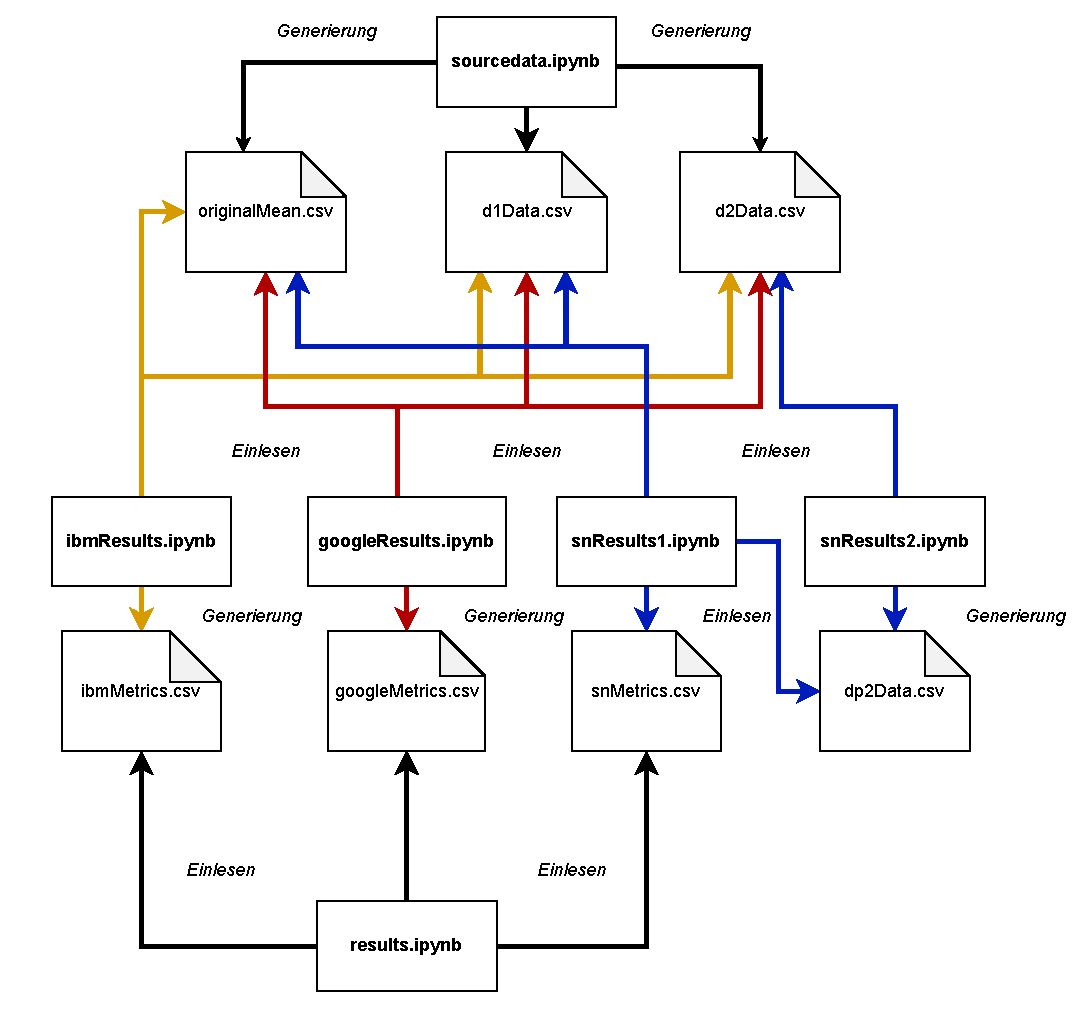
\includegraphics[scale=0.6]{./images/interface_overview.pdf}
	\caption{Eine Übersicht der generischen Schnittstelle für die Evaluation der Frameworks.}
	\label{fig:interface_overview}
\end{figure}

In diesen drei Dateien wird folgender \cref{noisedData} ausgeführt.
Nachdem die drei grundlegenden drei Dateien $d1Data$, $d2Data$ und originalMean gelesen sind, folgt darauf in der verschachtelten \textit{For-Schleife} die Berechnung der verrauschten Durchschnitte entsprechend der verschiedenen $\epsilon$ Werten. Diese sind für die Berechnungen der Metriken in Zeile 10 erforderlich. Jedes Framework berechnet ihre eigenen Metriken für die $\epsilon$-Werte und speichert sie in ihrer CSV-Datei ab. Bei dem Framework Smartnoise SDK liegt eine Besonderheit vor, da es zwei Dateien \textit{snResults1.ipynb} und \textit{snResults2.ipynb} verwendet. Hierbei wird lediglich die Berechnung der verrauschten Werte in Zeile 6 und 7 separiert in diesen Dateien berechnet. Somit kann die Berechnung parallel ausgeführt werden, da sonst die Laufzeit erheblich höher ist. Semantisch entsprechen sie gemeinsam dem Code in Zeile 1 bis 10.
\begin{algorithm}[t]
	\caption{Die Erzeugung der verrauschten Durchschnittswerte und die Berechnung aus ihnen resultierenden metrischen Werten}\label{noisedData}
	\begin{algorithmic}[1]
		\State $d1Data\gets read(d1Data.csv)$
		\State $d2Data\gets read(d2Data.csv)$
		\State $originalMean\gets read(originalMean.csv)$
		\For{$e$ $in$ $epsilons$}
		\For{$index=0$ $to$ $1000$}
		\State $noisedMean1\gets  dp.mean(d1Data)$
		\State $noisedMean2\gets  dp.mean(d2Data)$
		\EndFor
		\EndFor
		\State $metrics\gets calculateMetrics(noisedMean1,noisedMean2,originalMean)$
	\end{algorithmic}
\end{algorithm}
In der letzten Datei results.ipynb erfolgt lediglich die Veranschaulichung der Metriken gemeinsam in einem Diagramm. 

\section{Datenstruktur}
Für die Evaluation werden bestimmte Daten in CSV Dateien abgespeichert, damit die generische Schnittstelle flexibel und unabhängig von den Frameworks funktionieren kann.

Die drei CSV Dateien $d1Data$, $d2Data$ und $originalMean$ dienen als Grundbasis der Evaluation. Wenn diese neu berechnet werden, muss die gesamte Evaluation für einen Vergleich erneut durchgeführt werden. Damit dies nicht jedes Mal vom neuen erforderlich ist, werden sie einmal abgespeichert und von den Frameworks nur gelesen.

Die weitere Separierung der Frameworks in eigene Jupyter Notebooks und ihre Abspeicherung der Ergebnisse in CSV Dateien soll die Flexibilität unterstützen. Es können beliebig viele Durchläufe der \gls{dp} Berechnungen erfolgen, welche in den entsprechenden results.csv gespeichert werden (siehe \cref{fig:interface_overview}). In der Datei \textit{results.ipynb} werden alle Durchläufe zu jedem Framework in einem Array gespeichert. Je nach Auswahl des Arrayfeldes für ein bestimmtes Framework kann ein spezifischer Durchlauf veranschaulicht werden. Dies erleichtert den Vergleich der Werte aus den Metriken.

\section{Probleme}
Eine große Herausforderung dieser Arbeit war es geeignete Metriken für die Evaluation zu finden. Trotz intensiver Literaturrecherche bezüglich Papers im Bereich \gls{dp} wurden keine vergleichsweise Evaluationen wie diese gefunden. Nach genauerem Lesen wurden ein paar Papers im Bereich Analyse von \gls{dp} gefunden, die sich mit der Genauigkeit sowie Privatsphäre von \gls{dp} beschäftigten. Jedoch gab es keine expliziten in Bezug auf Frameworks. Nach langer Recherche wurde im Framework Smartnoise SDK eine Teilbibliothek gefunden, welche sich für Evaluation von \gls{dp} Algorithmen sich eignet \parencite{SNEVAL}. Hierbei werden 8 Metriken für die Evaluation eingesetzt. Diese wurden analysiert und beurteilt, ob sie für diese Bachelorarbeit sinnvoll und nutzbar sind. Dabei wurde bei Fachliteraturen in der Mathematik recherchiert und in Tests in Python auf Tauglichkeit überprüft. Davon wurden 5 Metriken übernommen.

In weiteren verschiedenen Veröffentlichungen wurde zur Bestimmung der Genauigkeit das Modell einer logistischen Regression verwendet. Diese galt als eine Möglichkeit die Auswirkung des Verrauschens auf Rohdaten zu beurteilen. Für diese Bachelorarbeit wurde ebenfalls dieses Modell in Python implementiert und veranschaulicht. Nach einigen Tests sowie Recherche folgte, dass das Szenario dieser Bachelorarbeit für dieses Modell zu einfach ist. Dies lag am Kriterium, welcher der originale Durchschnitt war. Das Modell konnte schnell dieses Kriterium lernen. Somit wurde eine Genauigkeit (score) von ca. 98\% stets erreicht. Aufgrund dessen hat die Aussagekraft für eine Beurteilung des Verrauschens gefehlt. Schließlich wurde dieses Modell für diese Arbeit nicht miteingebracht.

Eine große Hürde war die Feststellung der Gründe für die entgegen den Erwartungen auftretenden Ergebnisse. Die Frameworks beinhalten bekannte Mechanismen wie Laplace und weitere. Jedoch ist die Prozedur des Frameworks intern nicht von außen nachvollziehbar. Das Verrauschen folgt einem Mechanismus, welcher unterschiedlich implementiert werden kann. Um die Ergebnisse auf Richtigkeit und Gültigkeit zu prüfen, wurden neben den Ergebnissen auch Zwischenergebnisse der Berechnungen gespeichert. Diese halfen die Berechnungen der Frameworks besser nachzuvollziehen. Des Weiteren folgten in den Ergebnissen der Metriken Abweichungen aufgrund von kleinen $\epsilon$-Werten. Eine valide Beurteilung der Leistung des Frameworks wäre somit nicht möglich gewesen. Insgesamt konnte ein geeignetes Intervall an $\epsilon$-Werten sowie plausible Ergebnisse bestimmt werden. 

\chapter{Evaluation}
In diesem Kapitel wird auf das Ergebnis der drei Frameworks in den Kategorien Privatsphäre, Genauigkeit und Erwartungstreue eingegangen. Hierbei werden diese Ergebnisse veranschaulicht und in Anbetracht des erwarteten Ergebnisses beschrieben.

\section{Voraussetzungen}
Für diese Evaluation wurde die Menge an $\epsilon$-Werten [0,5;1,0;1,5;3,0;5,0] ausgewählt. Sie umfasst ein Spektrum an kleinen sowie großen Werten, wie sie in verschiedener wissenschaftlicher Literatur verwendet wird. Einerseits werden diese $\epsilon$-Werte in Anwendungen eingesetzt. Andererseits wird dadurch das Verhalten des Frameworks in Bezug zur Definition von \gls{dp} sicherer überprüft, da sich je nach der Größe des  $\epsilon$-Wertes die semantische Bedeutung des Ergebnisses ändern kann.

Die Evaluationsergebnisse sind in einigen Bereichen vom Wert her niedrig ausgefallen, die auf den einfachen medizinischen Anwendungsfall in dieser Arbeit zurückzuführen sind. Trotzdem ist die Aussagekraft sowie Validität vorhanden, da die Frameworks solche Fälle ebenfalls unterstützen und konsistent durch Zwischenergebnisse sind.

Die Metriken werten ein unveränderter Datensatz, der die Durchschnitte der Eingabewerte erhält, sowie die beiden mit DP verrauschten Datensätze \glqq Datensatz1 \grqq und \glqq Datensatz2 \grqq aus. Sie beinhalten jeweils 1000 Werte. Der unveränderte Durchschnittsdatensatz beinhaltet 1000 Mal den Durchschnitt aller Alterswerte der Rohdaten. \textbf{Dieser entspricht in diesem Fall dem Durchschnittsalter von 36.1 Jahren.} Die verrauschten Datensätze beinhalten die Ergebnisse von jeweils 1000 unabhängigen DP-geschützten Berechnungen des Durchschnittsalters pro $\epsilon$-Wert. Näheres dazu siehe Kapitel $4$.

Bei der Erläuterung der Ergebnisse wird auf Zwischenergebnisse hingewiesen. Sie sind der Durchschnitt für jeden $\epsilon$-Wert des verrauschten Datensatzes$1$ und Datensatzes$2$. In dieser Evaluation sind das 10 Werte insgesamt. Es gibt zwei verrauschte Datensätze mit jeweils 5 $\epsilon$-Werten. Diese dienen als Hilfe zur Erklärung der Ergebnisse der Metriken. 

Des Weiteren liegt der Fokus des Verständnisses der Ergebnisse in der Kategorie. Zwar sind übergreifende Erklärungen aufgrund von Zusammenhängen möglich, jedoch folgt dies verstärkt in den Folgerungen (Kapitel 7).

Als Grundlage der verrauschten Durchschnittsfunktion der Frameworks diente der Laplace Mechanismus, welcher für das Verrauschen der Daten zuständig ist.

Bei den Diagrammen werden Punkte angezeigt, die die tatsächlichen Ergebnisse der Metrik darstellen. Zur Verdeutlichung des Verlaufes sind Punkt zu Punktverbindungen durch gestrichelte Linien hinzugefügt worden.
\newpage

\section{Privatsphäre}
In diesem Abschnitt werden die Ergebnisse der Metriken DP-res und Wasserstein-Distanz evaluiert. Die erste Metrik überprüft die Einhaltung der \gls{dp} Definition. Die zweite bewertet die Qualität des Verrauschens der Frameworks für verschiedene $\epsilon$-Werte.
\subsection{DP-res}
Als erstes sollte in der Evaluation überprüft werden, ob die verwendeten Frameworks überhaupt in der Lage sind korrekt mit DP verrauschte Ergebnisse zu erzeugen. Hierbei bildeten die beiden verrauschten Datensätze die Eingabe.
\begin{table}[h]
	\centering
	\begin{tabular}{ l l l l} \toprule
		\textbf{Epsilon-Werte} & \textbf{IBM \gls{dp}} & \textbf{Google DP} & \textbf{Smartnoise SDK}  \\ \midrule
		0,5	& true  & true & true\\
		1,0 	& true  & true & true\\
		1,5 & true  & true & true\\
		3,0	& true  & true & true\\
		5,0   & true  & true & true\\ \bottomrule
	\end{tabular}
	\caption{Die Ergebnisse der DP-res Metrik für die $\epsilon$-Werte der drei Frameworks.}
	\label{tab :dp_res}
\end{table}

\textbf{Erwartetes Ergebnis:}
Jedes Ergebnis der Frameworks muss DP-res erfüllen, damit die Definition von \gls{dp} eingehalten wird. Also soll jedes der Frameworks bei seinen Ergebnissen stets true erhalten.

\textbf{IBM \gls{dp} Ergebnis:}
Alle Ergebnisse von IBM \gls{dp} erfüllten die Definition von \gls{dp}.

\textbf{Google Ergebnis:}
Alle Ergebnisse von Google erfüllten die Definition von \gls{dp}.

\textbf{Smartnoise SDK Ergebnis:}
Alle Ergebnisse von Smartnoise SDK erfüllten die Definition von \gls{dp}.
\newpage

\subsection{Wasserstein-Distanz}
Als nächstes wurde die Wasserstein-Distanz berechnet um, die Qualität des Verrauschens zu bewerten. Dafür war die Eingabe die zwei verrauschten Datensätze. Die Berechnung ist mehrmals erfolgt, um ein stabiles Ergebnis (kein Ausnahmeergebnis) zu erhalten. Da die Eingabe benachbarte Datensätze sind, wird wieder auf die Definition von \gls{dp} eingegangen. Das Gesamtergebnis ist in \cref{fig:wsd} zu betrachten.

\textbf{Erwartetes Ergebnis:}
Desto größer die Wasserstein-Distanz ist, desto unähnlicher sind die  Datensätze. Der umgekehrte Fall gilt ebenfalls. Daher wird erwartet, dass die Punkte entsprechend einer streng monoton fallenden Kurve verlaufen. Dies bedeutet dann, dass bei einem kleinen $\epsilon$-Wert die Ähnlichkeit der Datensätze sehr gering ist, sodass die Privatsphäre vermehrt geschützt wird. Bei einem steigenden $\epsilon$-Wert hingegen nimmt die Ähnlichkeit der Datensätze zu, wodurch die Privatsphäre abnimmt. Dies entspricht der Definition von \gls{dp}, die auf zwei benachbarten Datensätzen basiert.

\begin{figure}[htbp]
	\centering
	\subfloat[Das Ergebnis von IBM \gls{dp} für die Wasserstein-Distanz.]{
		\label {fig:ibm_wsd}
		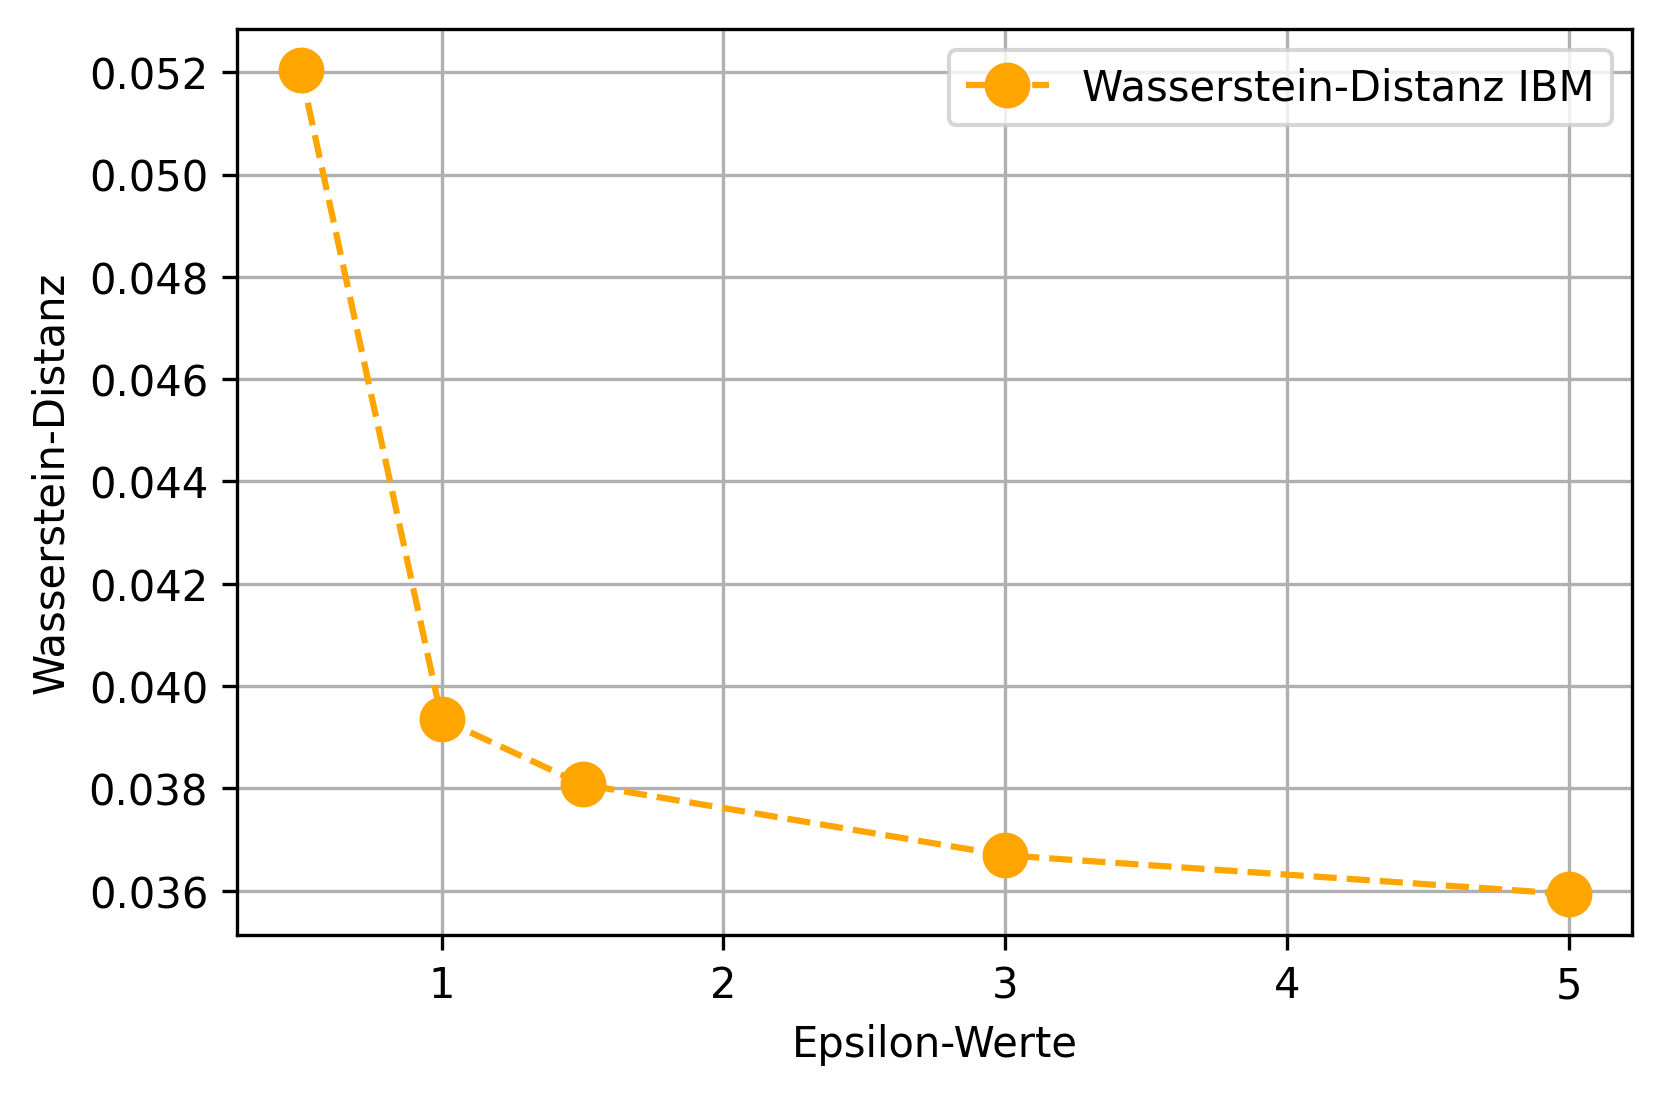
\includegraphics[scale=0.4]{./images/ibm_wsd.png}
	} \qquad
	\subfloat[Das Ergebnis von Google für die Wasserstein-Distanz.]{
		\label {fig:google_wsd}
		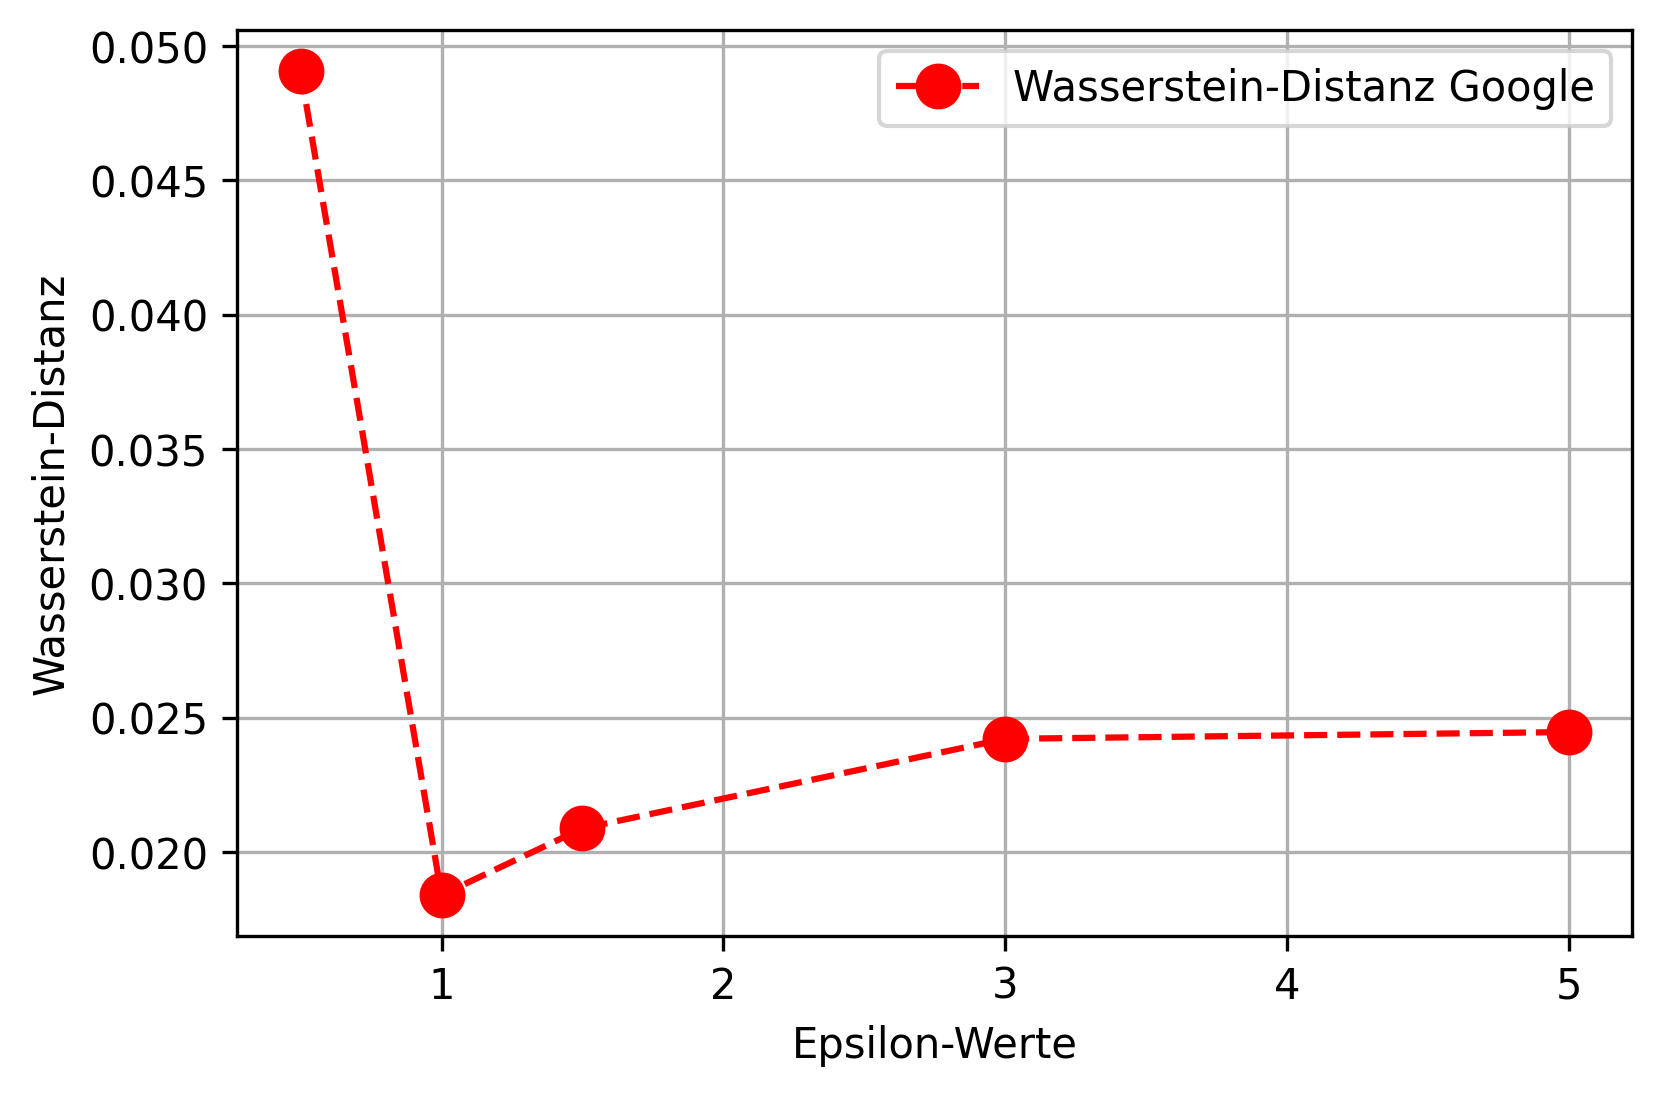
\includegraphics[scale=0.4]{./images/google_wsd.png}
	}
	\subfloat[Das Ergebnis von Smartnoise SDK für die Wasserstein-Distanz.]{
		\label {fig:sn_wsd}
		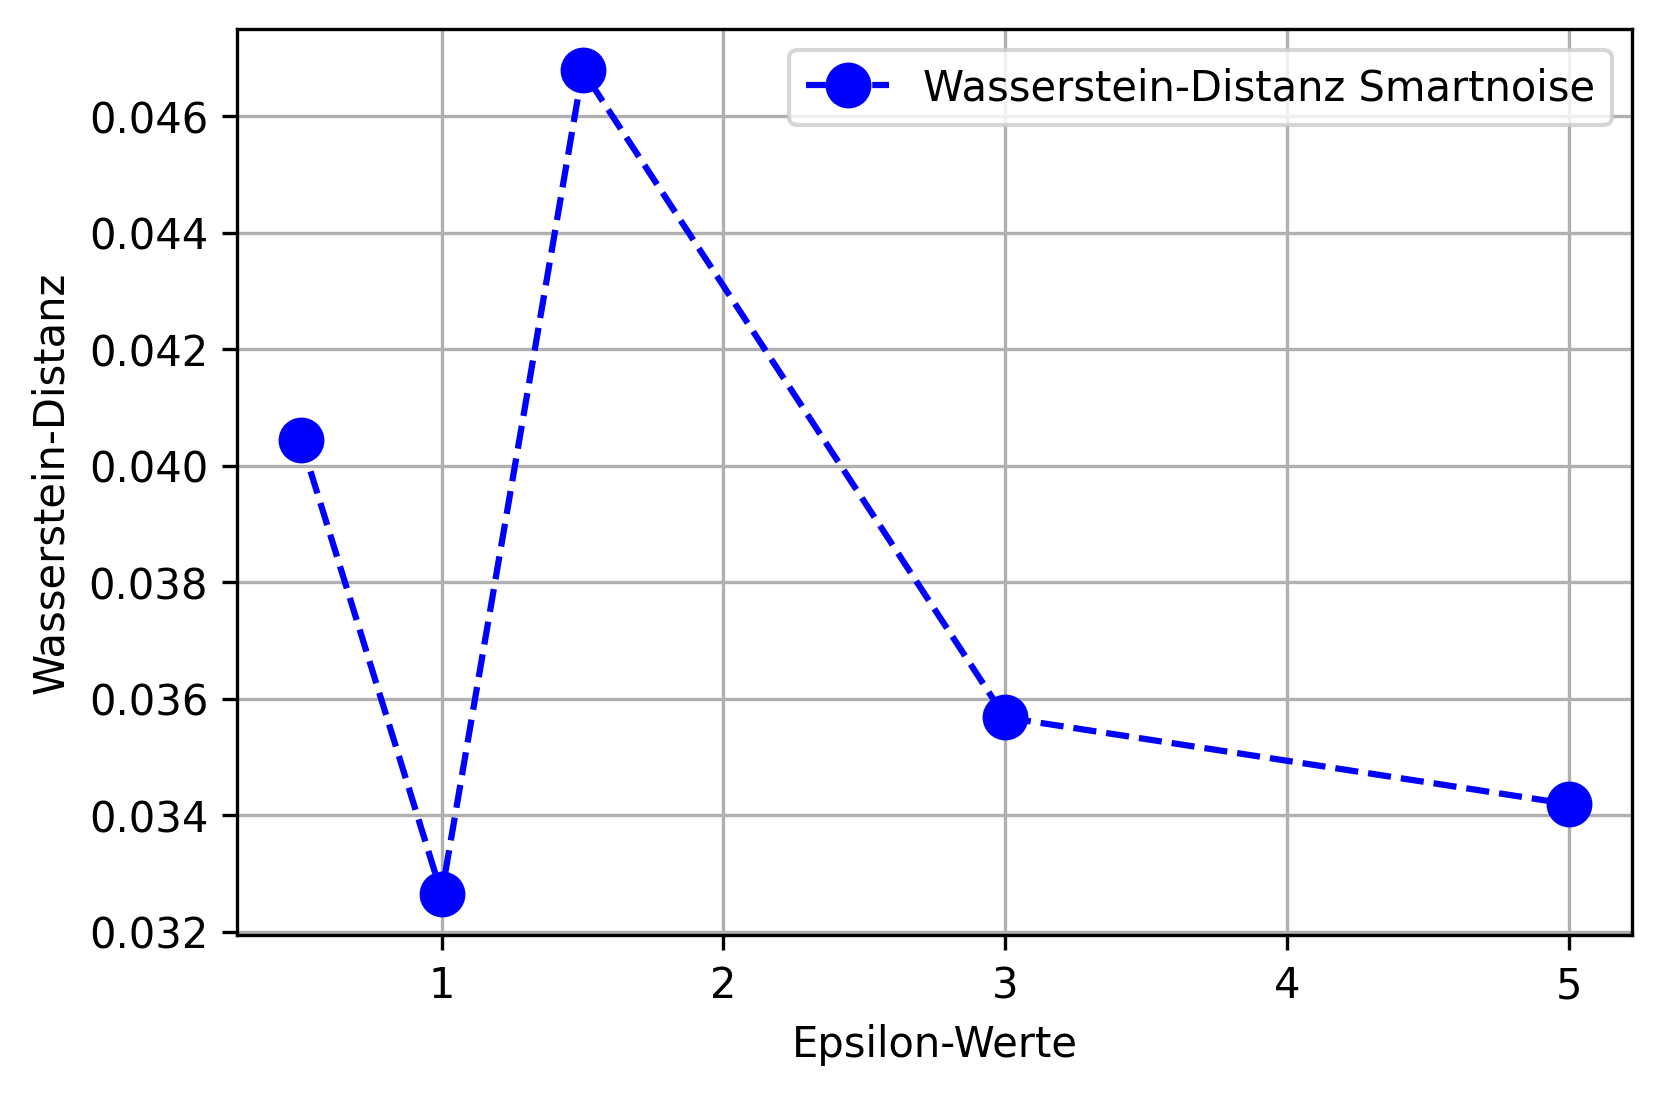
\includegraphics[scale=0.4]{./images/sn_wsd.png}
	}
	\caption{Die Ergebnisse der Wasserstein-Distanz für die $\epsilon$-Werte [0,5;1,0;1,5;3,0;5,0] der drei Frameworks.}
	\label{fig:wsd}
\end{figure}


\textbf{IBM \gls{dp} Ergebnis:}
Das Ergebnis entsprach den Erwartungen. In der \cref{fig:ibm_wsd} wird eine streng monoton fallende Kurve ersichtlich. Sie hat den Höchstwert der Wasserstein Distanz für den kleinsten $\epsilon$-Wert und das Minimum für den größten $\epsilon$-Wert. Die Differenz zwischen ihnen liegt bei ca. 0,015, sodass die Privatsphäre in einem relativ großem Wertebereich geschützt wird. Die Abnahme der Distanz erfolgt in Relation zum $\epsilon$-Wert gleichmäßig. Ab dem $\epsilon$-Wert 3,0 konvergiert der Wert der Distanz gegen ca. 0,0370. Daraus folgt ein Mindestwert der Wasserstein-Distanz für die Daten, somit ein Mindestniveau für den Schutz der Privatsphäre.

\textbf{Google Ergebnis:}
Das Ergebnis in \cref{fig:google_wsd} entsprach nicht einer streng monoton fallenden Kurve. Beim kleinsten $\epsilon$-Wert erreicht es einen hohen Wert. Dies stimmt noch mit der Erwartung überein. Anschließend folgen zwei Ausreißer für die $\epsilon$-Werte 1,0 und 1,5. Hierbei ist die Metrik deutlich niedriger als der vorherige Punkt ausgefallen. Die Differenz zwischen dem ersten und dem zweiten Punkt liegt bei ca. 0,03. Im weiteren Verlauf der Kurve bei dem $\epsilon$-Werten 3,0 und 5,0 steigt sie leicht an und konvergiert gegen einen Wert von ca. 0,0248. Die durchschnittliche Wasserstein-Distanz von 0,029 liegt nahe an diesem.

Die Privatsphäre wird für den kleinsten $\epsilon$-Wert sorgfältig geschützt, anschließend findet ein rapider Abfall des Schutzniveaus statt. Dies birgt gewisse Unsicherheiten bei kleinen $\epsilon$-Werten, bei denen hauptsächlich der Fokus auf der Privatsphäre liegt und diese vermehrt eingehalten werden müsste.

Die Ausreißer lassen sich anhand der Zwischenergebnisse erklären. Die Differenz der $\epsilon$-Werte 1,0 und 1,5 sind bei den verrauschten Datensätzen gering, somit liegen sie nah beieinander. Das Verrauschen der Durchschnitte fiel somit bei diesen $\epsilon$-Werten geringer aus, als beim $\epsilon$-Wert 0,5. Hierbei war die Differenz beim Zwischenergebnis viel höher, ein deutliches Verrauschen geht hieraus hervor. Durch diese Zwischenergebnisse ist festgestellt, dass das unerwartete Verhalten der Kurve auf das Framework zurückzuführen ist. 
In diesem Framework folgen verschiedene Berechnungen für den Laplace Mechanismus, welcher für das Verrauschen verantwortlich ist, die als außenstehender nicht verständlich sind. Daher ist das Ergebnis teils unerklärbar, da die Zuweisung des Verrauschens auf die Rohdaten vom Framework ausgeht.

\textbf{Smartnoise SDK Ergebnis:}
Die ersten drei Punkte der $\epsilon$-Werte widersprechen den Erwartungen wie in \cref{fig:sn_wsd} ersichtlich. Der erste Punkt ist nicht der Höchstpunkt der Kurve. Dieser liegt beim dritten Punkt mit 0,0468 vor. Der zweite Punkte ist der Tiefpunkt der Kurve, sodass die Privatsphäre hierbei sehr gering geschützt ist. Ab dem dritten Punkt ist der Verlauf streng monoton fallend und entspricht somit der Erwartung. Beim ersten Punkt liegt der Wert zwischen dem zweite und dritten, da die Differenz der Zwischenergebnisse im Verhältnis zu den anderen dazwischen liegt. Hier war das Verrauschen im Verhältnis zum zweiten Punkt deutlich mehr, jedoch zum dritten Punkt geringer.

Die Zwischenergebnisse spiegeln die unerwartete Verteilung der drei ersten Punkte in der Metrik wieder. Diese Werte sind für die beiden Datensätze am $\epsilon$-Wert 1 sehr nah beieinander, wofür das geringe Verrauschen des Frameworks verantwortlich ist. Daraus folgt der niedrige Schutz der Privatsphäre. Dagegen beim $\epsilon$-Wert 1,5 ist die Differenz zwischen den Zwischenergebnissen höher als zuvor, wodurch die Metrik ein hohen Wert hat. Dieses Verhalten ist auf die den Laplace Mechanismus im Framework zuzuweisen. Er agiert hier nicht entsprechend der Definition von \gls{dp}. Dies ist eine Implementierungsangelegenheit, die entscheidet wie stark das Verrauschen ist, die lediglich vom Nutzer angewendet und beurteilt werden kann.

\begin{figure}[htbp]
	\centering
	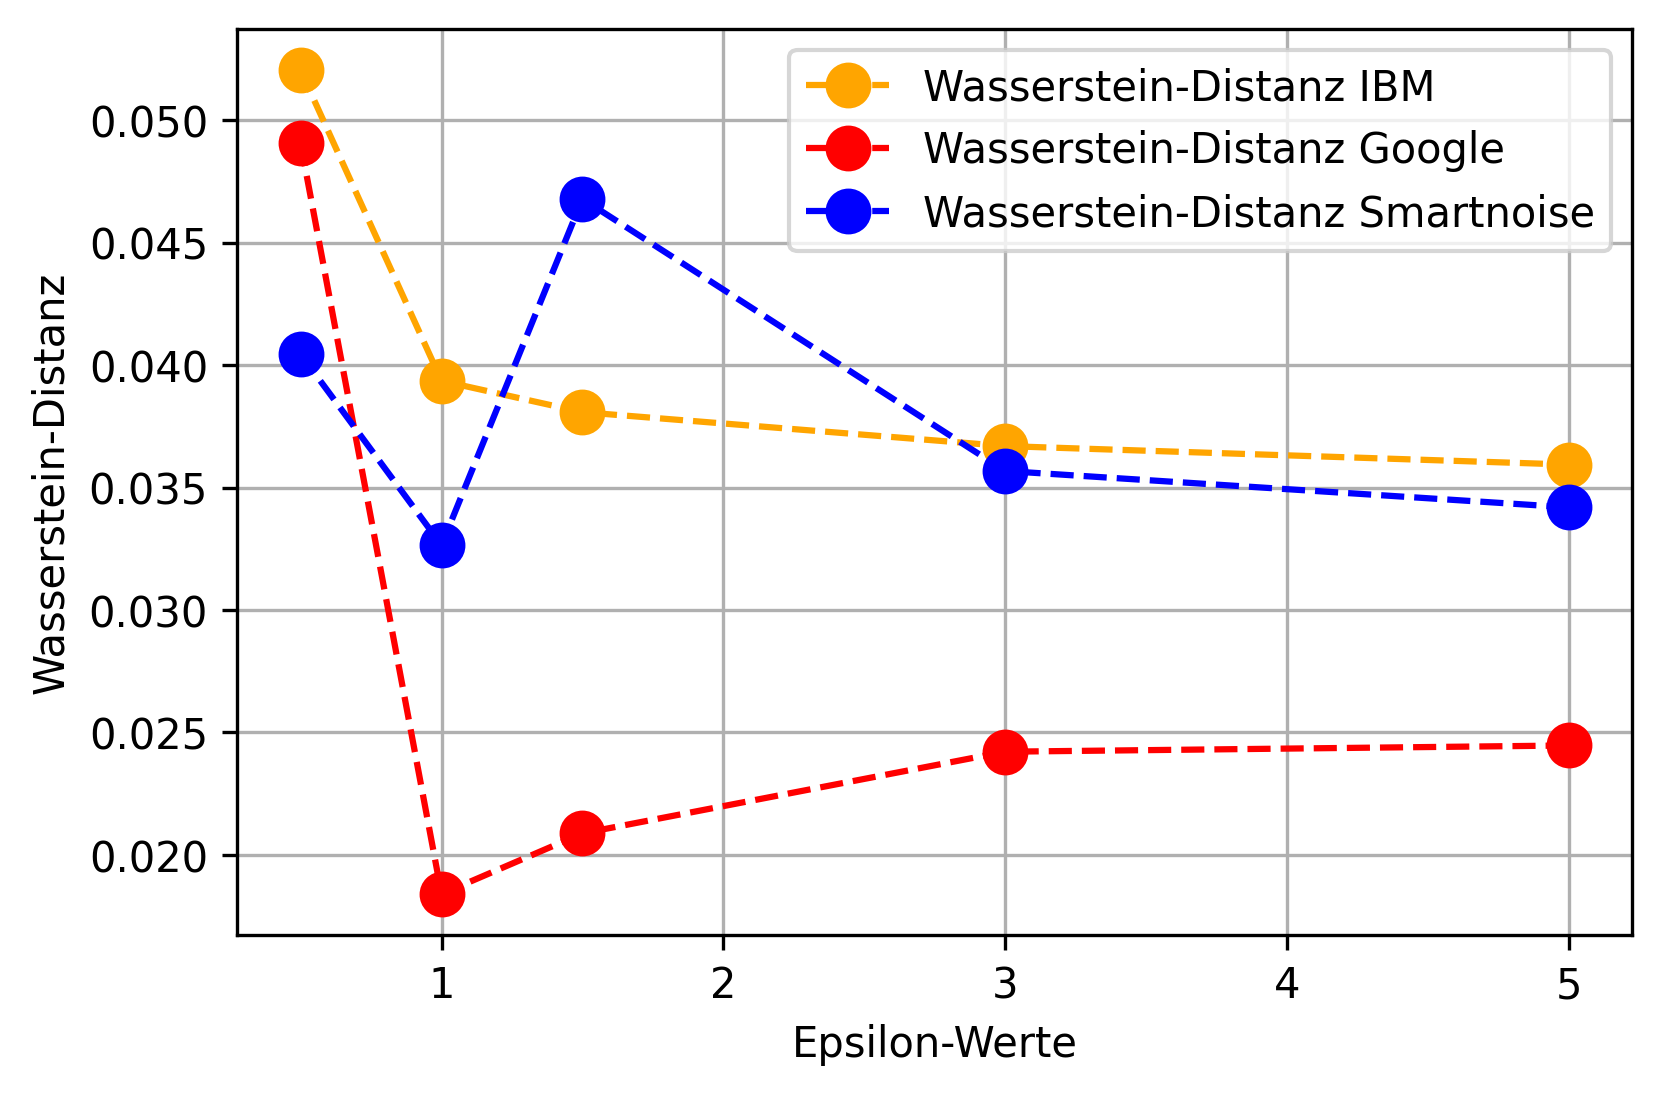
\includegraphics[scale=0.6]{./images/together_wsd.png}
	\caption{Die Gesamtübersicht der drei Frameworks in der Metrik Wasserstein-Distanz.}
	\label{fig:together_wsd}
\end{figure}

\textbf{Vergleich: }
In \cref{fig:wsd} werden die Ergebnisse der drei Frameworks in Vergleich gesetzt. Beim ersten $\epsilon$-Wert liegt bei jedem Framework außer beim Smartnoise SDK der Höchstwert vor. Ab diesem Punkt fällt der Wert der restlichen Punkte bei Google \gls{dp} in Gegensatz zu den anderen erheblich ab. Sie verläuft ohne eine Überschneidung unterhalb der anderen Frameworks zu haben. Die Kurve von IBM \gls{dp} hat insgesamt den Höchstwert und verläuft von diesem streng monoton fallend weiter. Sie behält bis zum $\epsilon$-Wert 5 stets den höchsten Wert für die Metrik außer beim $\epsilon$-Wert 1.5, hier liegt das Ergebnis von Smartnoise SDK höher. Ab dem vierten Punkt verlaufen die Ergebnisse dieser zwei Frameworks (IBM \gls{dp} und Smartnoise SDK) sehr nah beieinander, was für eine Konvergenz des Schutzes für die Privatsphäre bedeutet. Um ca. 0,01 liegt parallel dazu die Ergebnisse von Google vor. Insgesamt verlaufen die Kurven von IBM \gls{dp} und Smartnoise SDK im mittlerer oberer Bereich in Gegensatz zu Google im unteren.

Die Privatsphäre wird unterschiedlich stark bei den Frameworks geschützt. Beim IBM \gls{dp} ist ein stets hohes Niveau an Privatsphäre vorhanden. Dieser konvergiert ebenfalls auf einem hohen Niveau für große $\epsilon$-Werte. Somit ist ein hoher Schutz der Rohdaten vorhanden. Dagegen beim Google \gls{dp} fällt das Niveau des Schutz nach dem ersten Punkt erheblich. Vor allem bei kleinen $\epsilon$-Werten kann das Framework nicht einen hohen Schutz an Privatsphäre aufrechterhalten und hat in diesen den geringsten Schutz an Privatsphäre. Im Nachgang konvergiert es für weitere steigende $\epsilon$-Werte, jedoch auf dem niedrigsten Niveau in Verhältnis zu den restlichen Frameworks. Smartnoise SDK zeigt ein Verhalten auf, welches zwischen den beiden anderen liegt. Zum einen geht eine Instabilität bei den ersten drei Punkten hervor, die trotz dessen ein hohen Schutz an Privatsphäre anbieten. Zum anderen liegt die Konvergenz des Frameworks fast auf dem selben des IBM \gls{dp}, welches in bei kleinen $\epsilon$-Werten besser abschneidet.
\newpage
\section{Genauigkeit}
In diesem Abschnitt werden die Ergebnisse auf ihre Genauigkeit des Wertes zum unveränderten Datensatz beurteilt. Zu einem gibt die mittlere quadratische Abweichung ein Einblick auf die Auswirkung des Verrauschens. Zum anderen verschafft die Standardabweichung die Erkenntnis, inwieweit die Mechanismen stabil die Werte im Verhältnis zu den $\epsilon$-Werten Verrauschen. 

\subsection{Mittlere quadratische Abweichung}
Bei der mittleren quadratischen Abweichung war die Eingabe der erste verrauschte und der unveränderte Datensatz. Der Wert zeigt eine Tendenz des Frameworks auf, ob das Verrauschen verstärkt oder vermindert eingesetzt wird.

\textbf{Erwartetes Ergebnis:}
Desto größer die mittlere quadratische Abweichung ist, desto ungenauer sind die verrauschten Daten. Der umgekehrte Fall gilt ebenfalls. Das Ergebnis soll mit steigendem $\epsilon$-Wert genauer werden.
\begin{figure}[htbp]
	\centering
	\subfloat[Das Ergebnis von IBM \gls{dp} für die mittlere quadratische Abweichung.]{
		\label {fig:ibm_mse}
		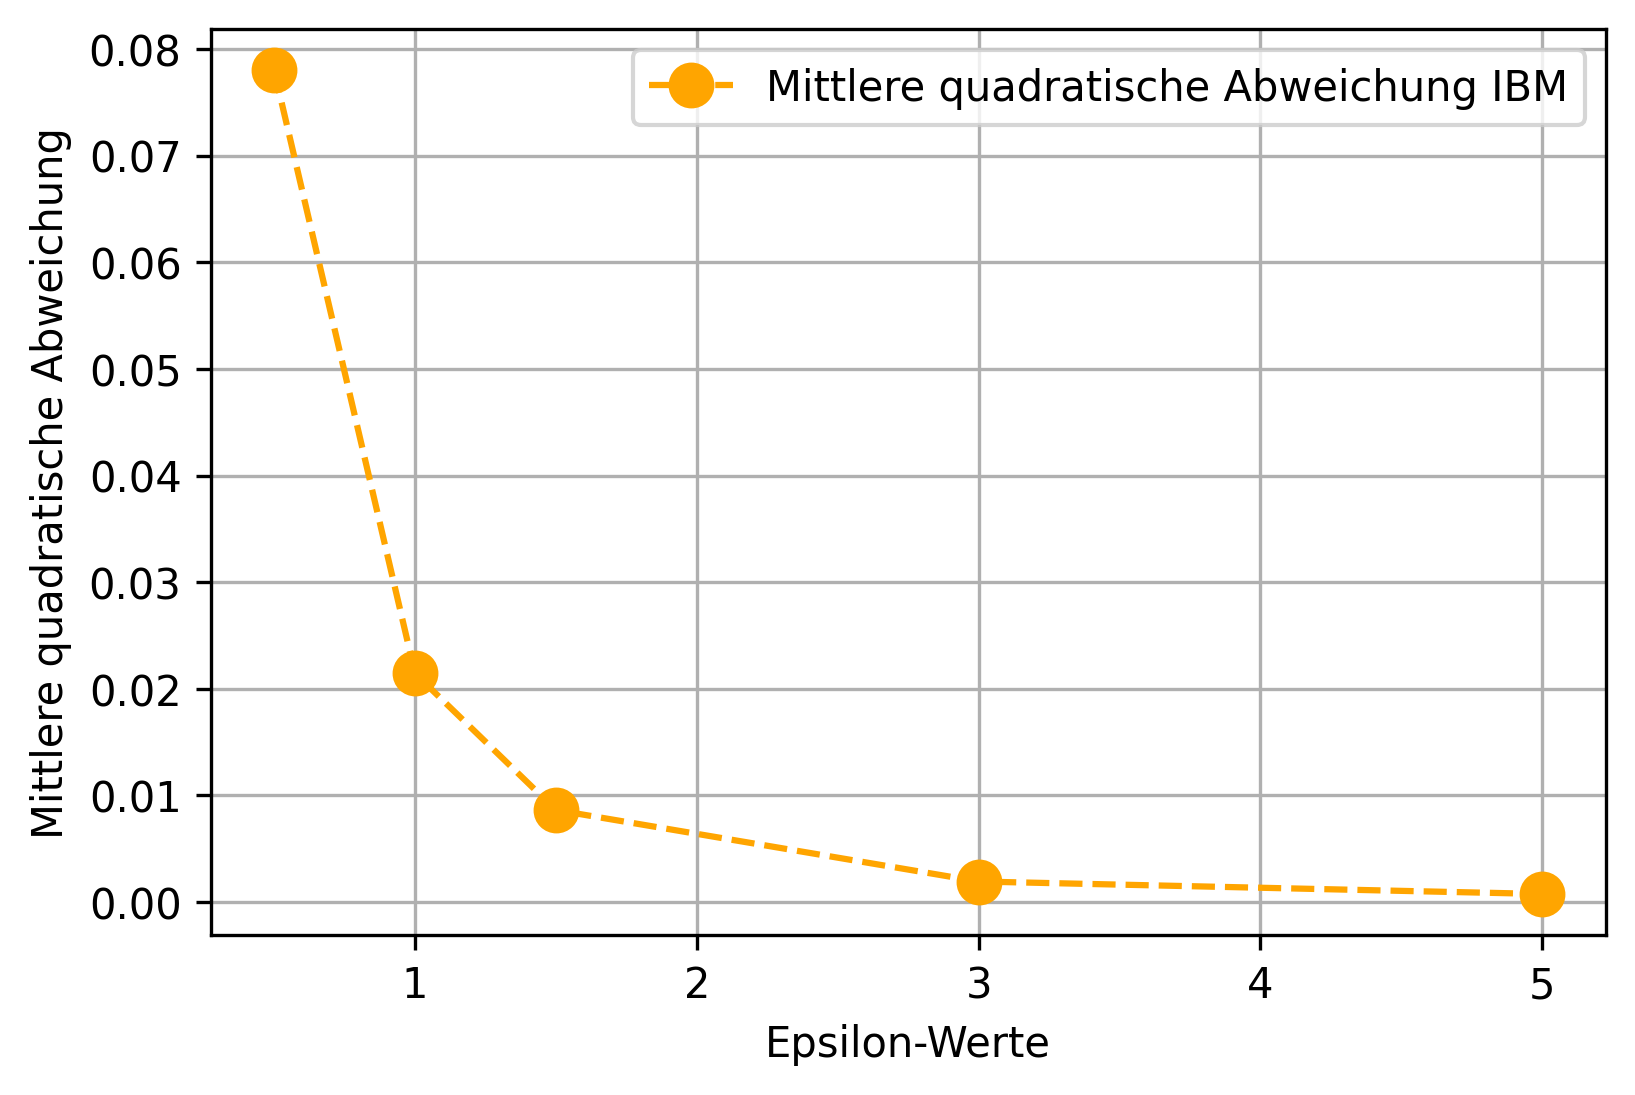
\includegraphics[scale=0.4]{./images/ibm_mse.png}
	} \qquad
	\subfloat[Das Ergebnis von Google für die mittlere quadratische Abweichung.]{
		\label {fig:google_mse}
		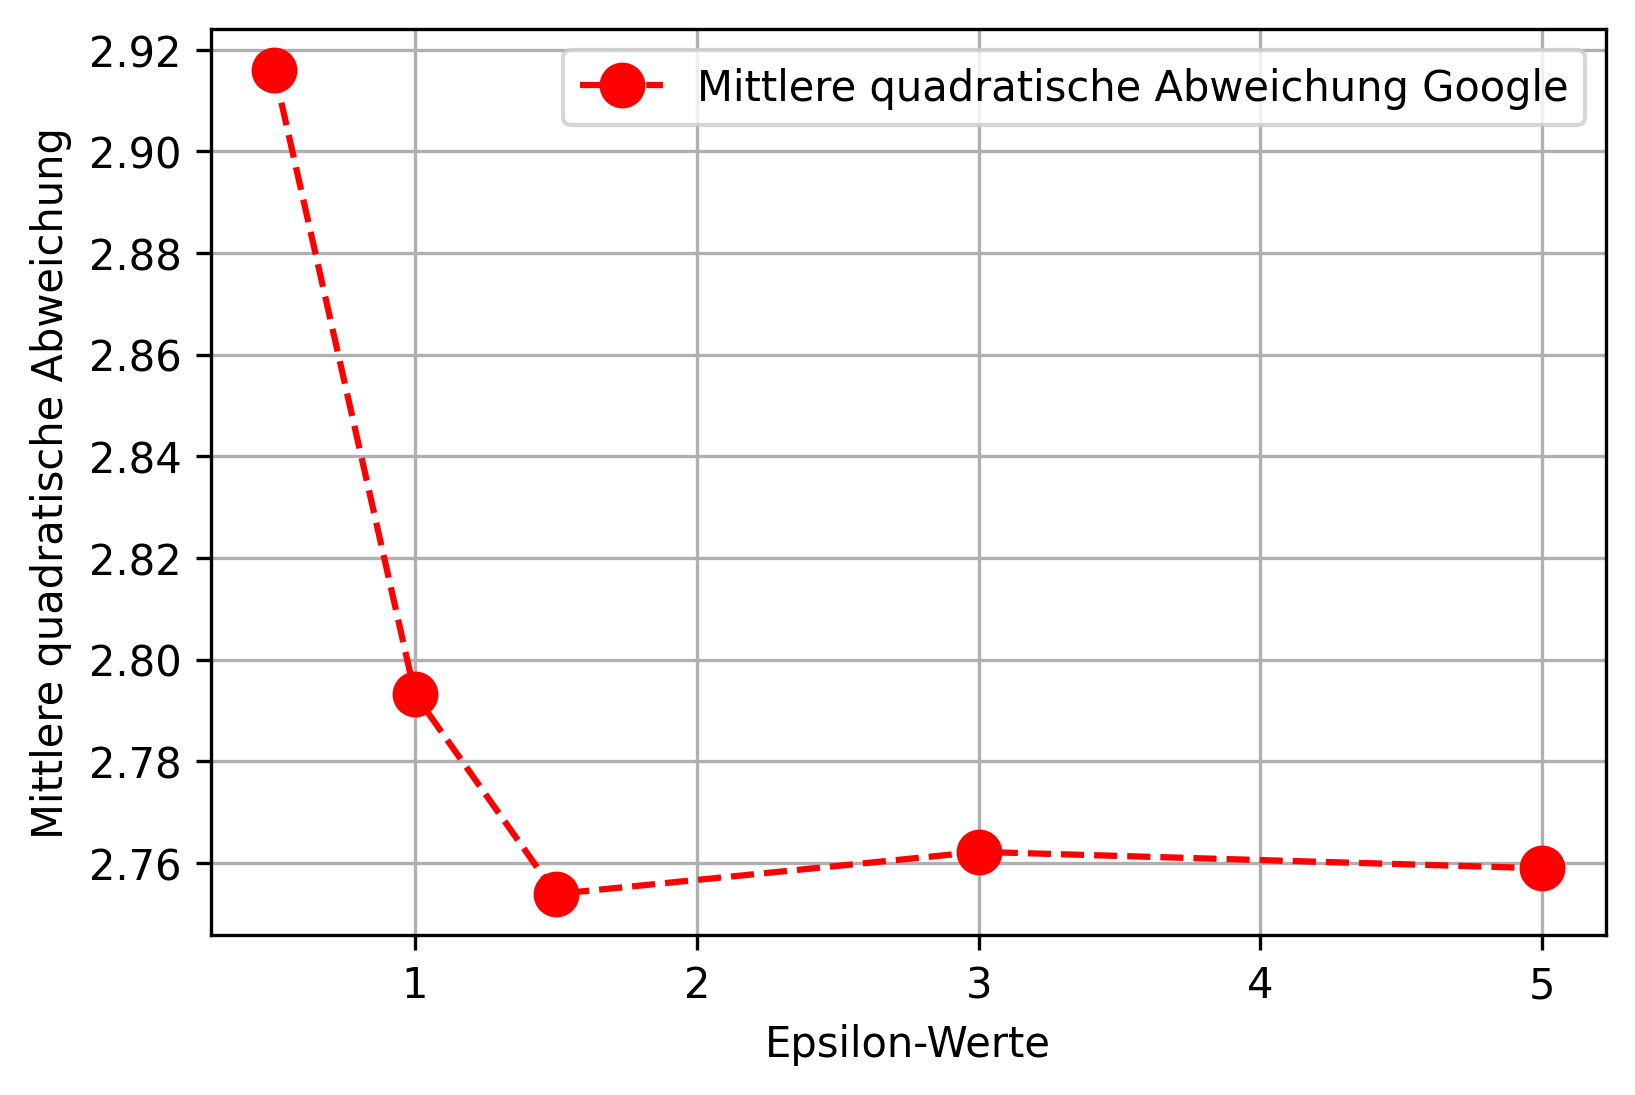
\includegraphics[scale=0.4]{./images/google_mse.png}
	}
	\subfloat[Das Ergebnis von Smartnoise SDK für die mittlere quadratische Abweichung.]{
		\label {fig:sn_mse}
		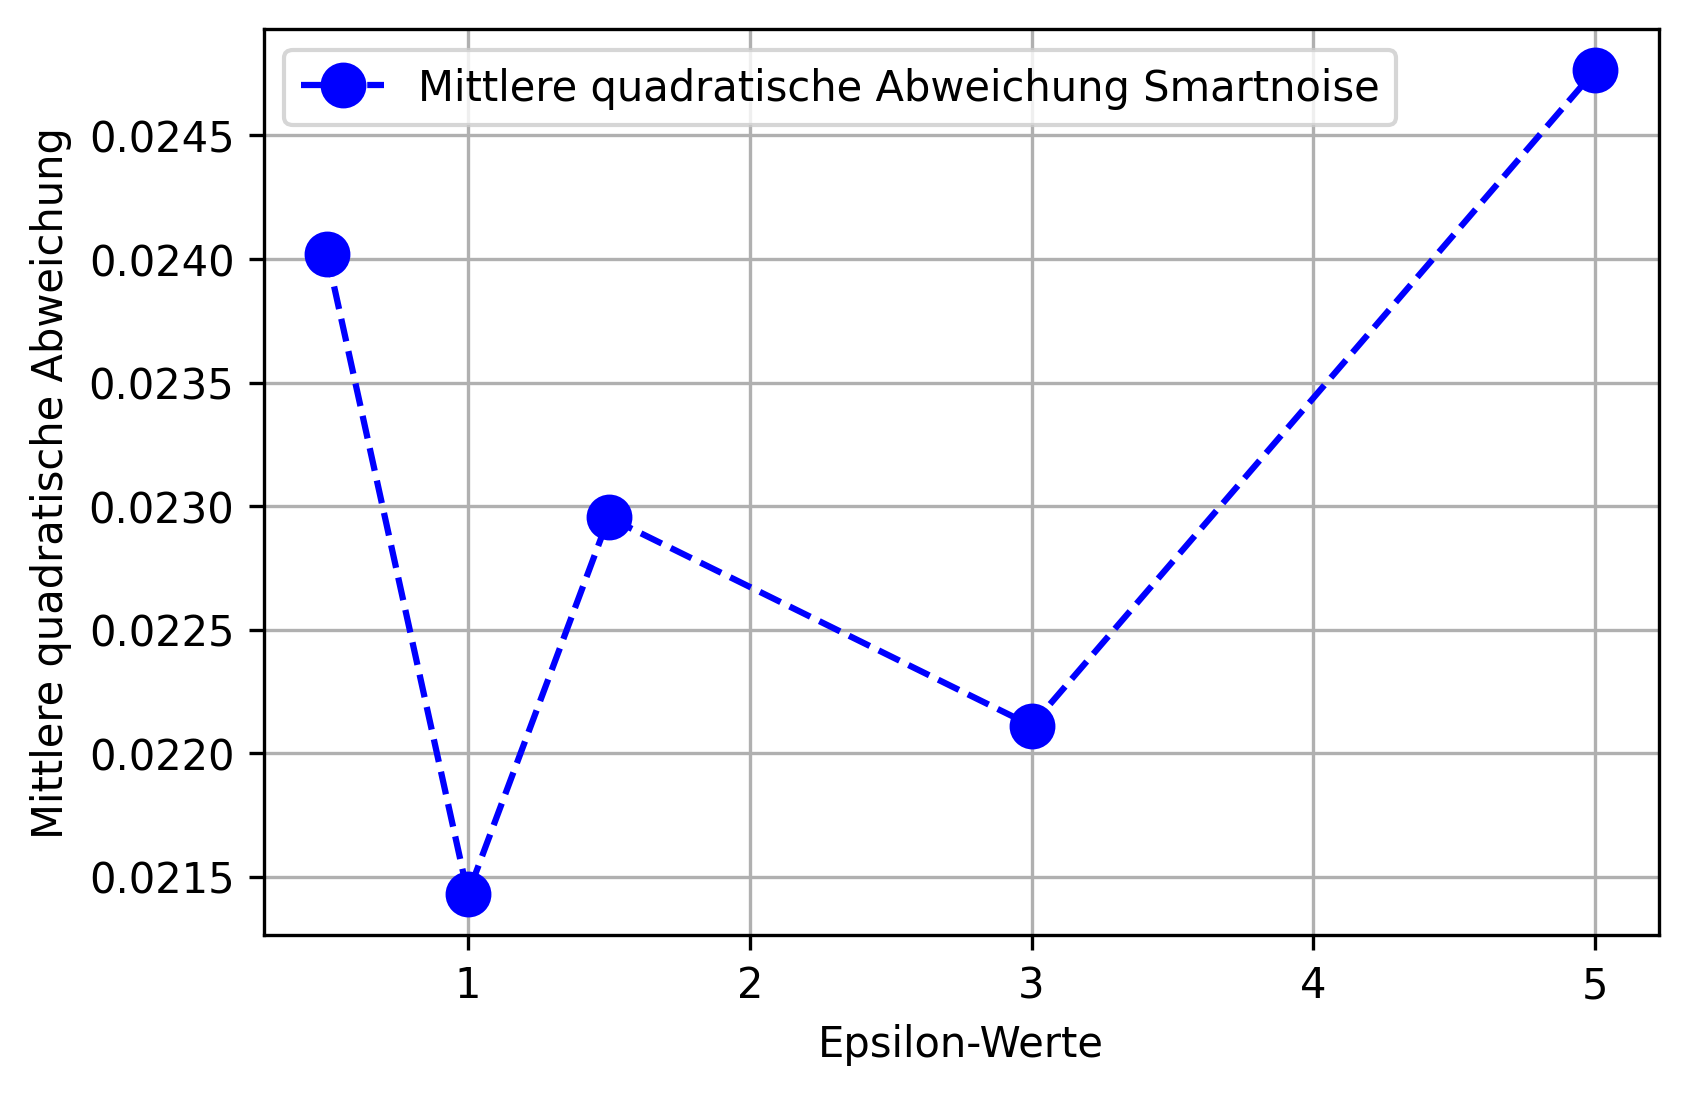
\includegraphics[scale=0.4]{./images/sn_mse.png}
	}
	\caption{Die Ergebnisse der mittleren quadratischen Abweichung der drei Frameworks für die $\epsilon$-Werte [0,5;1,0;1,5;3,0;5,0].}
	\label{fig:mse}
\end{figure}

\textbf{IBM \gls{dp} Ergebnis:}
Die Genauigkeit nimmt mit steigendem $\epsilon$-Wert zu, die fallende Kurve entspricht der Erwartung wie in \cref{fig:ibm_mse} ersichtlich. Ein Gesamtblick auf die Werte der Metrik zeigt eine hohe Genauigkeit auf. Vom ersten bis zum letzten Punkt steigt die Genauigkeit fast um das achtfache. Schon beim zweiten Punkt ist die Genauigkeit sehr gestiegen und der verrauschte Durchschnitt des Frameworks übereinstimmt fast mit dem des unveränderten beim fünften Punkt.

In den Zwischenergebnissen wird diese Auswertung deutlich, da diese sich nur in den Nachkommastellen zum originalen Durchschnittswert 36,1 variieren. Somit kann eine hohe Genauigkeit beobachtet werden.

\textbf{Google Ergebnis:}
Das Ergebnis in \cref{fig:google_mse} entspricht bis auf den 4 Punkt der Erwartung. Die Kurve hat ihren Höchstpunkt beim $\epsilon$-Wert 0,5 und sinkt mit steigendem $\epsilon$-Wert. Die weiteren Punkt nehmen einen niedrigeren Wert für die Abweichung an. Beim vierten Punkt ist der Wert minimal höher als der vorherige und nachherige, wodurch die strenge Monotonie unterbrochen wird. Ebenfalls ist ab diesem Punkt eine Konvergenz ersichtlich, sodass für weitere höhere $\epsilon$-Werte diese Metrik um den Wert 2.76 betragen würde.

Der unveränderte Durchschnitt beträgt 36.1 und in den Zwischenergebnisse hat der verrauschten Durchschnitt ca. den Wert 34. Er ist stets niedriger und nimmt mit steigendem $\epsilon$-Wert wie erwartet nicht zu. Dies weist ein internes Verhalten auf, welches als negatives Rauschen in den Zwischenergebnissen zum Vorschein kommt. Dies erklärt den hohen Wert für die mittlere quadratische Abweichung, wodurch eine hohe Ungenauigkeit vorliegt. Die verrauschten Werte haben eine weite Entfernung zu den originalen, welche sogar für große $\epsilon$-Werte nicht abnimmt, sondern stagniert. Diese weite Distanz ist vom Laplace Mechanismus vorgegeben, die unveränderbar ist. Das Framework berechnet das Hinzufügen des Rauschens nach seinen eigenen Vorgaben, sodass dieses Phänomen nachzuvollziehen erfordert eine tiefstgehende Untersuchung, was nicht Bestandteil dieser Bachelorarbeit ist und es in der Ausgabe fest vorhanden ist.

\textbf{Smartnoise SDK Ergebnis:}
Das Ergebnis in \cref{fig:sn_mse} besitzt am zweiten sowie fünften Punkt einen Ausreißer. Der Höchstpunkt liegt nicht am ersten sondern am fünften, sodass die höchste Ungenauigkeit beim größten anstatt am kleinsten $\epsilon$-Wert vorliegt. Beim zweiten Punkt handelt es sich um den Tiefstpunkt der Ungenauigkeit, welcher beim fünften liegen sollte. Da sonst am zweiten Punkt, bei einem kleinen $\epsilon$-Wert eine höhere Genauigkeit als an den anderen Punkten zutrifft.

In den Zwischenergebnissen liegen die verrauschten Durchschnitte um den originalen Durchschnittswert 36.1, weswegen die Werte der Metrik gering ausgefallen sind. Des Weiteren verursacht die randomisierte Zuweisung des Verrauschens vom Laplace Mechanismus für die Ausreißer. Hierbei liegen die Zwischenergebnisse sehr nah beieinander, sodass die Unterschiede in den Nachkommastellen deutlich werden. Dies kann der Grund für die fehlende strenge Monotonie sein. Kleine Abweichungen in ihnen verursachen große Schwankungen in den Metriken, welche stärker als bei unterschiedlichen $\epsilon$-Werten. Insgesamt sorgt das Framework für eine sehr hohe Genauigkeit für kleine sowie große $\epsilon$-Werte. Ein erheblicher erwartete Unterschied zwischen den verschiedenen $\epsilon$-Werten ist nicht erkenntlich.
\begin{figure}[!htbp]
	\centering
	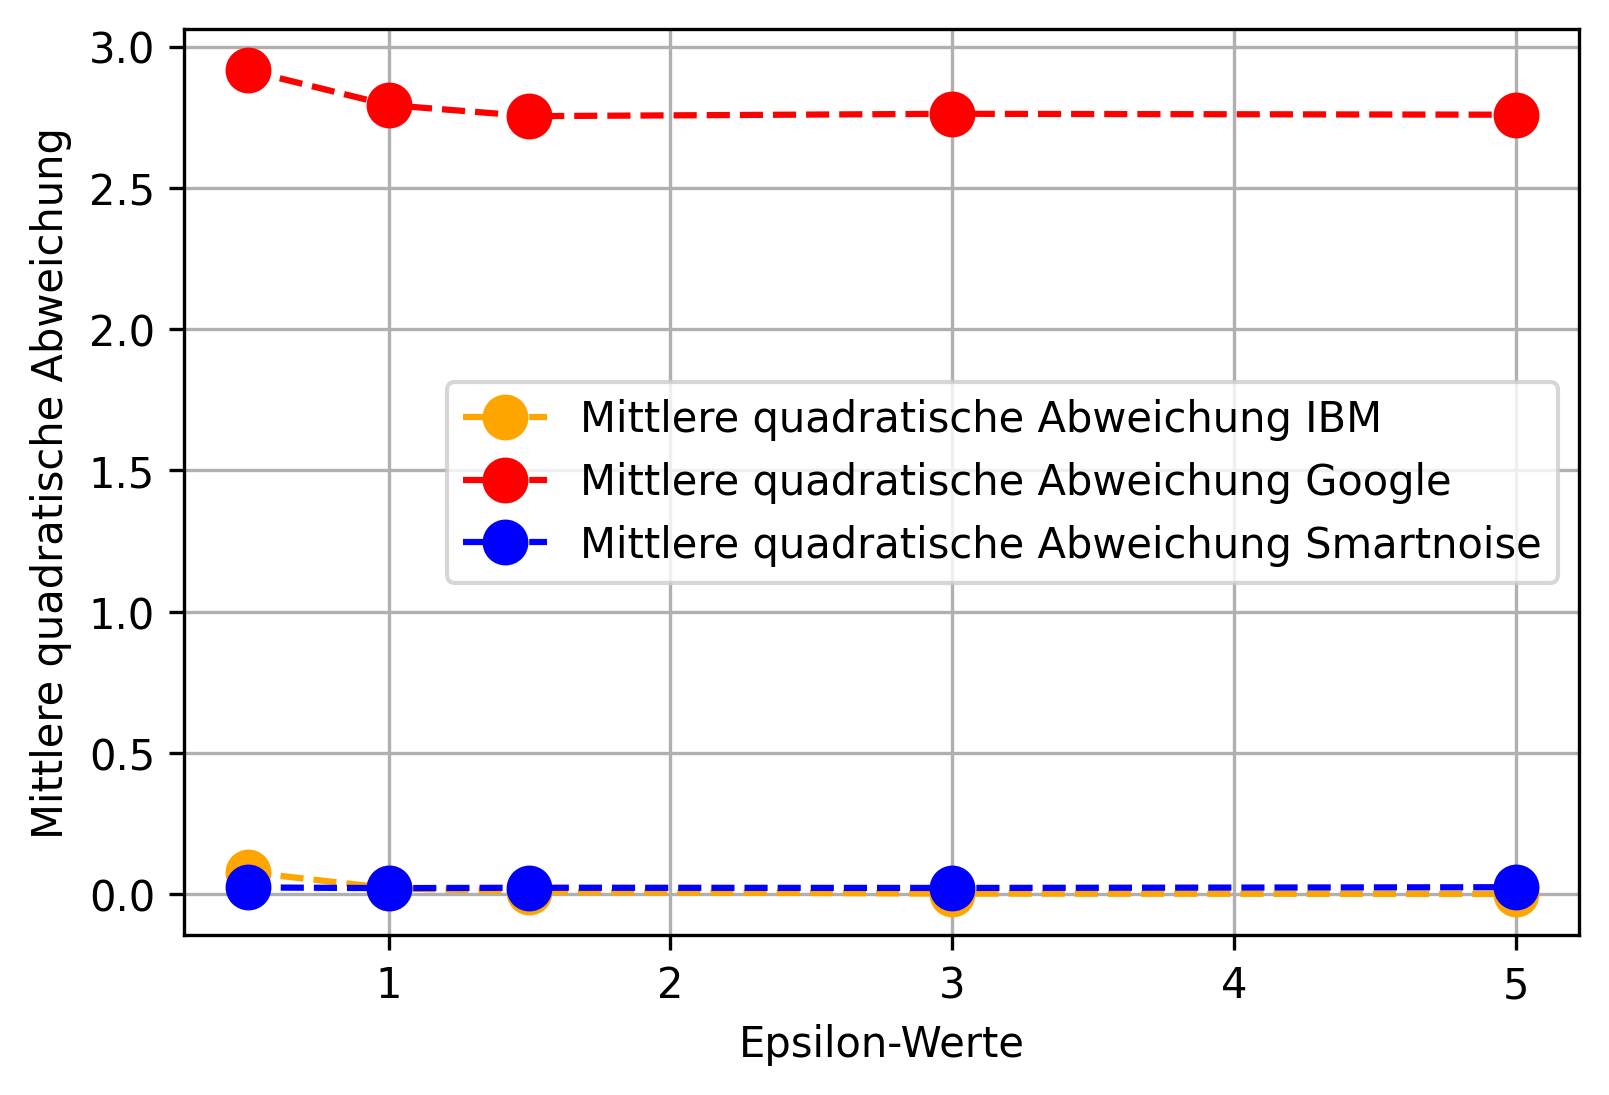
\includegraphics[scale=0.6]{./images/together_mse.png}
	\caption{Die Gesamtübersicht der drei Frameworks in der Metrik Mittlere quadratische Abweichung.}
	\label{fig:together_mse}
\end{figure}

\textbf{Vergleich: }
Im Gesamtüberblick in \cref{fig:together_mse} wird der Grad der Genauigkeit der Frameworks eindeutig erkennbar. IBM \gls{dp} und Smartnoise SDK befinden sich nahe des Wertes $0$ für die Metrik. Aus dieser Perspektive ist keine erkenntliche Unterscheidung zwischen kleinen und großen $\epsilon$-Werten in der Genauigkeit sichtbar. Daher ist die Beurteilung von IBM \gls{dp} und Smartnoise SDK in der zu vorigen spezifischen Beschreibungen eindeutig. Hier kann das Verhältnis zu einander analysiert werden.
Die Kurve von Google sticht zu den anderen deutlich hervor. Sie ist wie die beiden von IBM \gls{dp} und Smartnoise SDK im Gesamten konstant und verläuft um den Wert 3. Dieser weist auf eine durchgehende hohe Ungenauigkeit der verrauschten Daten hin. In Relation zu den anderen sorgt das Verrauschen vom Google Laplace Mechanismus für einen zu niedrigen Wert. Sein Rauschen ist im Allgemeinen zu stark.

\subsection{Standardabweichung}
Anhand der Standardabweichung wird die Stabilität der Genauigkeit des Laplace Mechanismus bestimmt. Dafür ist lediglich der erste verrauschte Datensatz als Eingabe notwendig.

\textbf{Erwartetes Ergebnis:}
Die Abweichung der Werte um den Mittelwert weißt auf die Sorgfalt des Mechanismus hin. Wenn eine große Abweichung bei kleinen $\epsilon$-Werten vorliegt, dann ist die Privatsphäre besser geschützt, jedoch nimmt die Stabilität der Genauigkeit ab. Die höhere Abweichung sorgt für verschiedene verrauschte Werte, die damit insgesamt ihre Genauigkeit senkt. Im umgekehrten Fall gilt dies ebenfalls. Vor allem bei großen $\epsilon$-Werten ist eine hohe Stabilität in der Genauigkeit zu erwarten, da dann der Mechanismus weniger Rauschen dazu addiert.

\begin{figure}[htbp]
	\centering
	\subfloat[Das Ergebnis von IBM \gls{dp} für die Standardabweichung.]{
		\label {fig:ibm_std}
		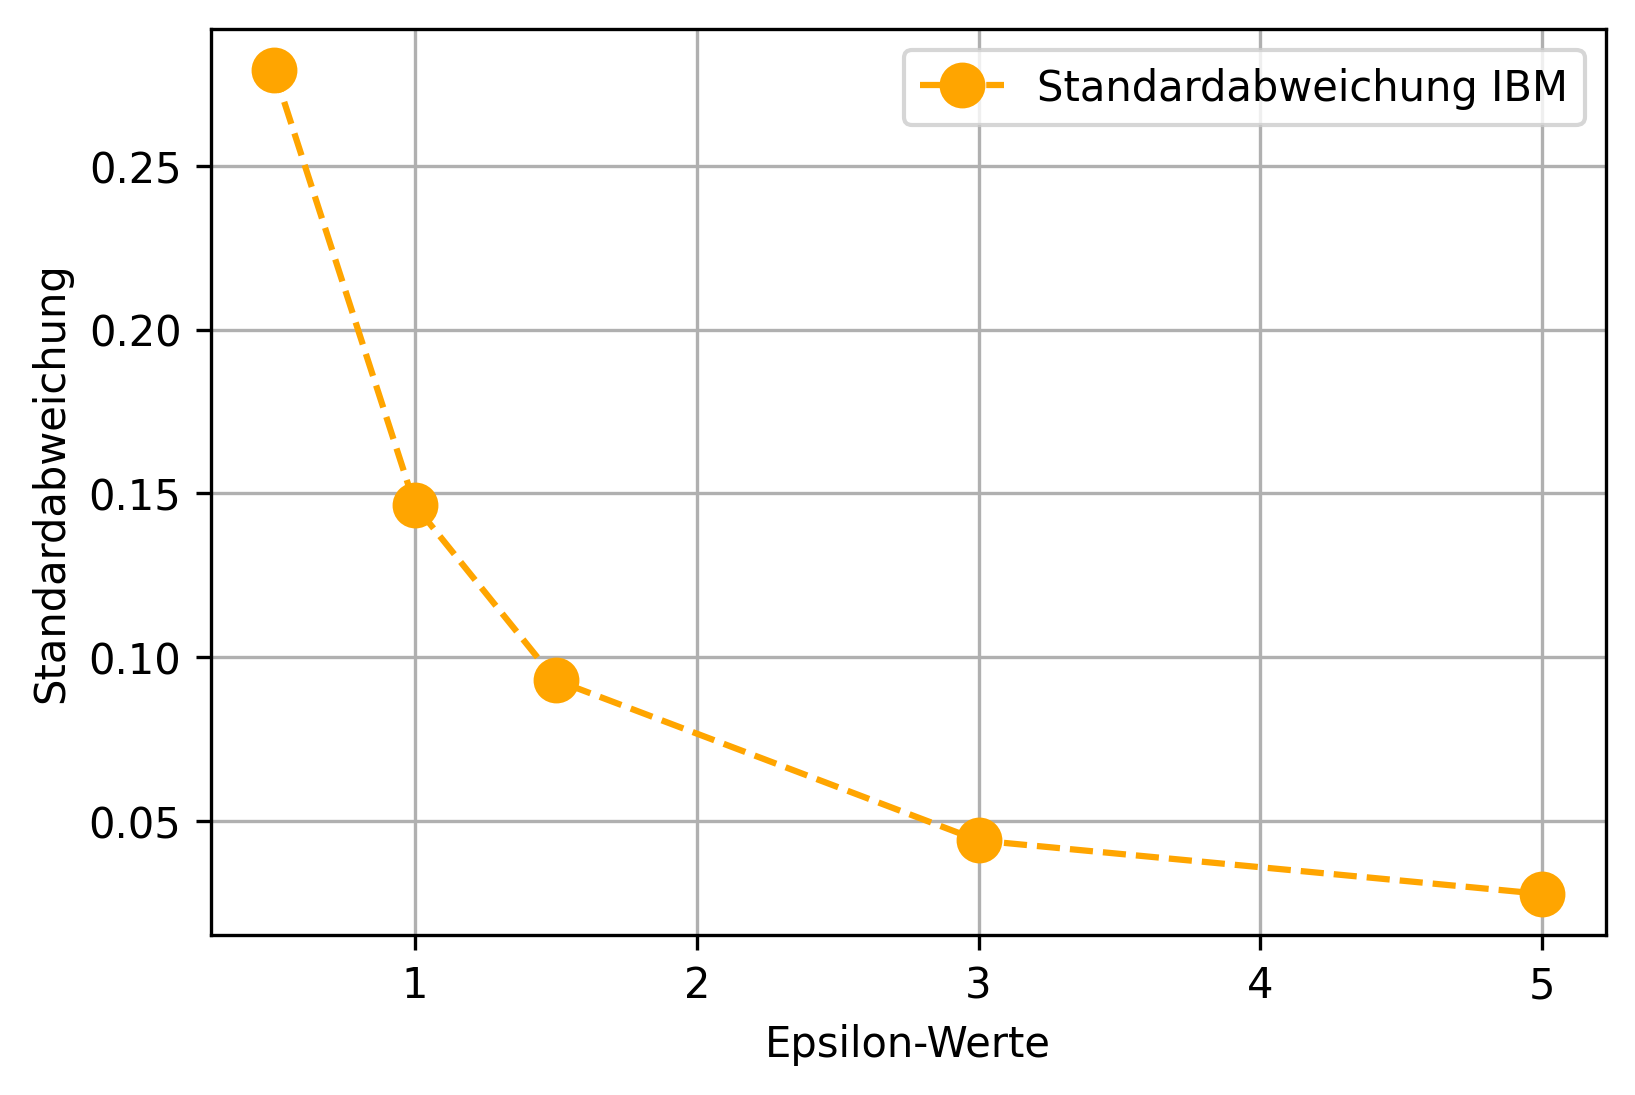
\includegraphics[scale=0.4]{./images/ibm_std.png}
	} \qquad
	\subfloat[Das Ergebnis von Google für die Standardabweichung.]{
		\label {fig:google_std}
		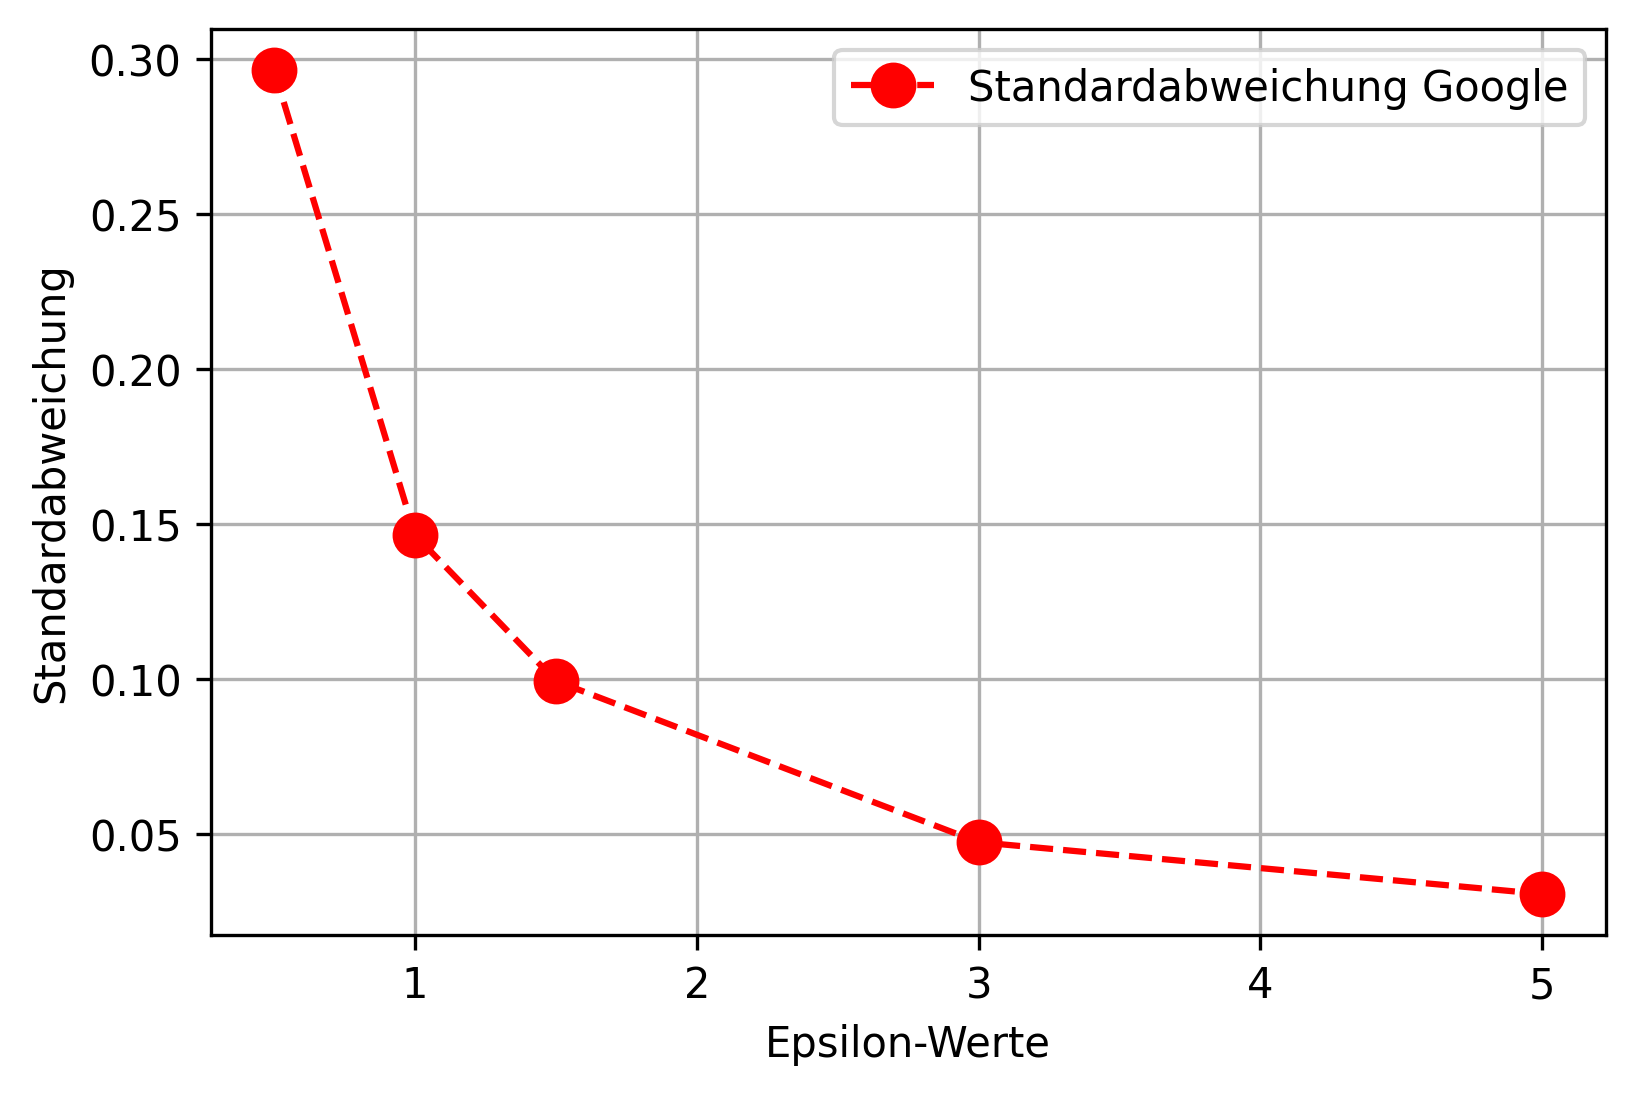
\includegraphics[scale=0.4]{./images/google_std.png}
	}
	\subfloat[Das Ergebnis von Smartnoise SDK für die Standardabweichung.]{
		\label {fig:sn_std}
		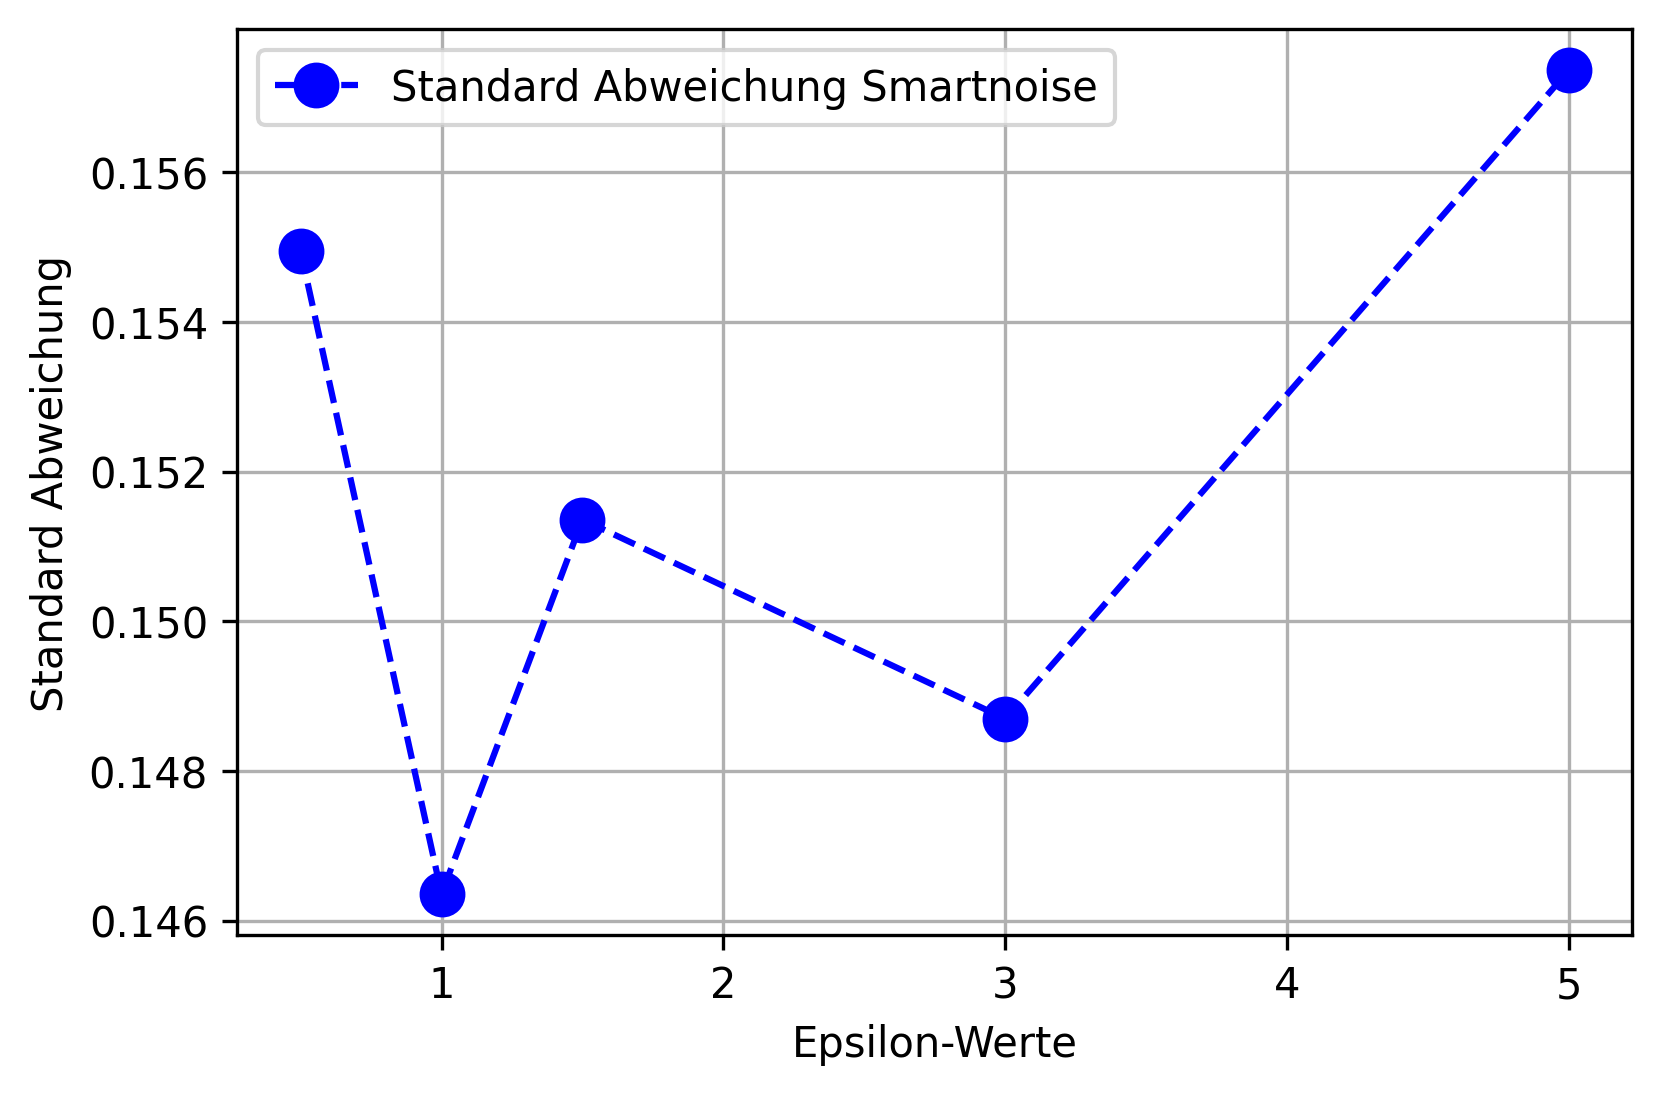
\includegraphics[scale=0.4]{./images/sn_std.png}
	}
	\caption{Die Ergebnisse der Standardabweichung für die $\epsilon$-Werte [0,5;1,0;1,5;3,0;5,0] der drei Frameworks.}
	\label{fig:std}
\end{figure}

\textbf{IBM \gls{dp} Ergebnis:}
Bei diesem Ergebnis in \cref{fig:ibm_std} spricht die streng monoton fallende Kurve für eine zunehmende Stabilität bei steigendem $\epsilon$-Wert. Dieses Verhalten entspricht der Definition von \gls{dp}. Für einen kleinen $\epsilon$-Wert wird die Privatsphäre mehr geschützt und die Genauigkeit dafür vernachlässigt, daher sind die Ausgaben variierter.Dies spiegelt sich in den ersten drei Punkten wieder. Die letzten zwei Punkte sprechen für eine hohe Stabilität der verrauschten Daten, da der Wert sehr nahe bei $0$ liegt. Somit wird kaum noch die Werte stärker verrauscht.

\textbf{Google Ergebnis:}
Die Kurve erfolgt den Erwartungen streng monoton fallenden wie in \cref{fig:google_std} erkennbar zu sein. Bei kleinen $\epsilon$-Werten ist die Abweichung höher als bei größeren. Dies deutet auf eine größere Instabilität in der Ausgabe bei kleinen $\epsilon$-Werten. Der Wertebereich der Metrik nimmt um ein Sechstel ab, was eine hohe Präzision des Mechanismus aufzeigt. Er agiert bei kleinen sowie großen $\epsilon$-Werten stets richtig. Auffallend sind die letzten zwei Punkte, welche sehr nahe an $0$ liegen. Dafür wird vom Laplace Mechanismus nur Verrauschen in den Nachkommastellen hinzugefügt, welche nicht mehr signifikant die Werte ändern. In den Zwischenergebnissen wird dies deutlich, da sie sich hauptsächlich in den Nachkommastellen (4-7 Stelle) unterscheiden.

\textbf{Smartnoise SDK Ergebnis:}
Insgesamt verläuft die Kurve in \cref{fig:sn_std} nicht streng monoton und keinem erkenntlichen Schema. Für die Beurteilung der Stabilität genügen die Werte der Metrik für eine Analyse. Die Werte weichen leicht in einem Rahmen von ca. 0,007 vom Mittelwert 0,151 ab. Dies erweist ein Stagnieren der Abweichung. Es existiert keine signifikante Differenz zwischen dem niedrigsten und höchstem $\epsilon$-Wert. Der Laplace Mechanismus fügt somit stets im gleichen Maße an Verrauschen hinzu. Die Qualität der Stabilität in der Genauigkeit bleibt erhalten und fällt bei verschiedene $\epsilon$-Werte gleich aus. Sie entspricht einer Konstanten.
\begin{figure}[htbp]
	\centering
	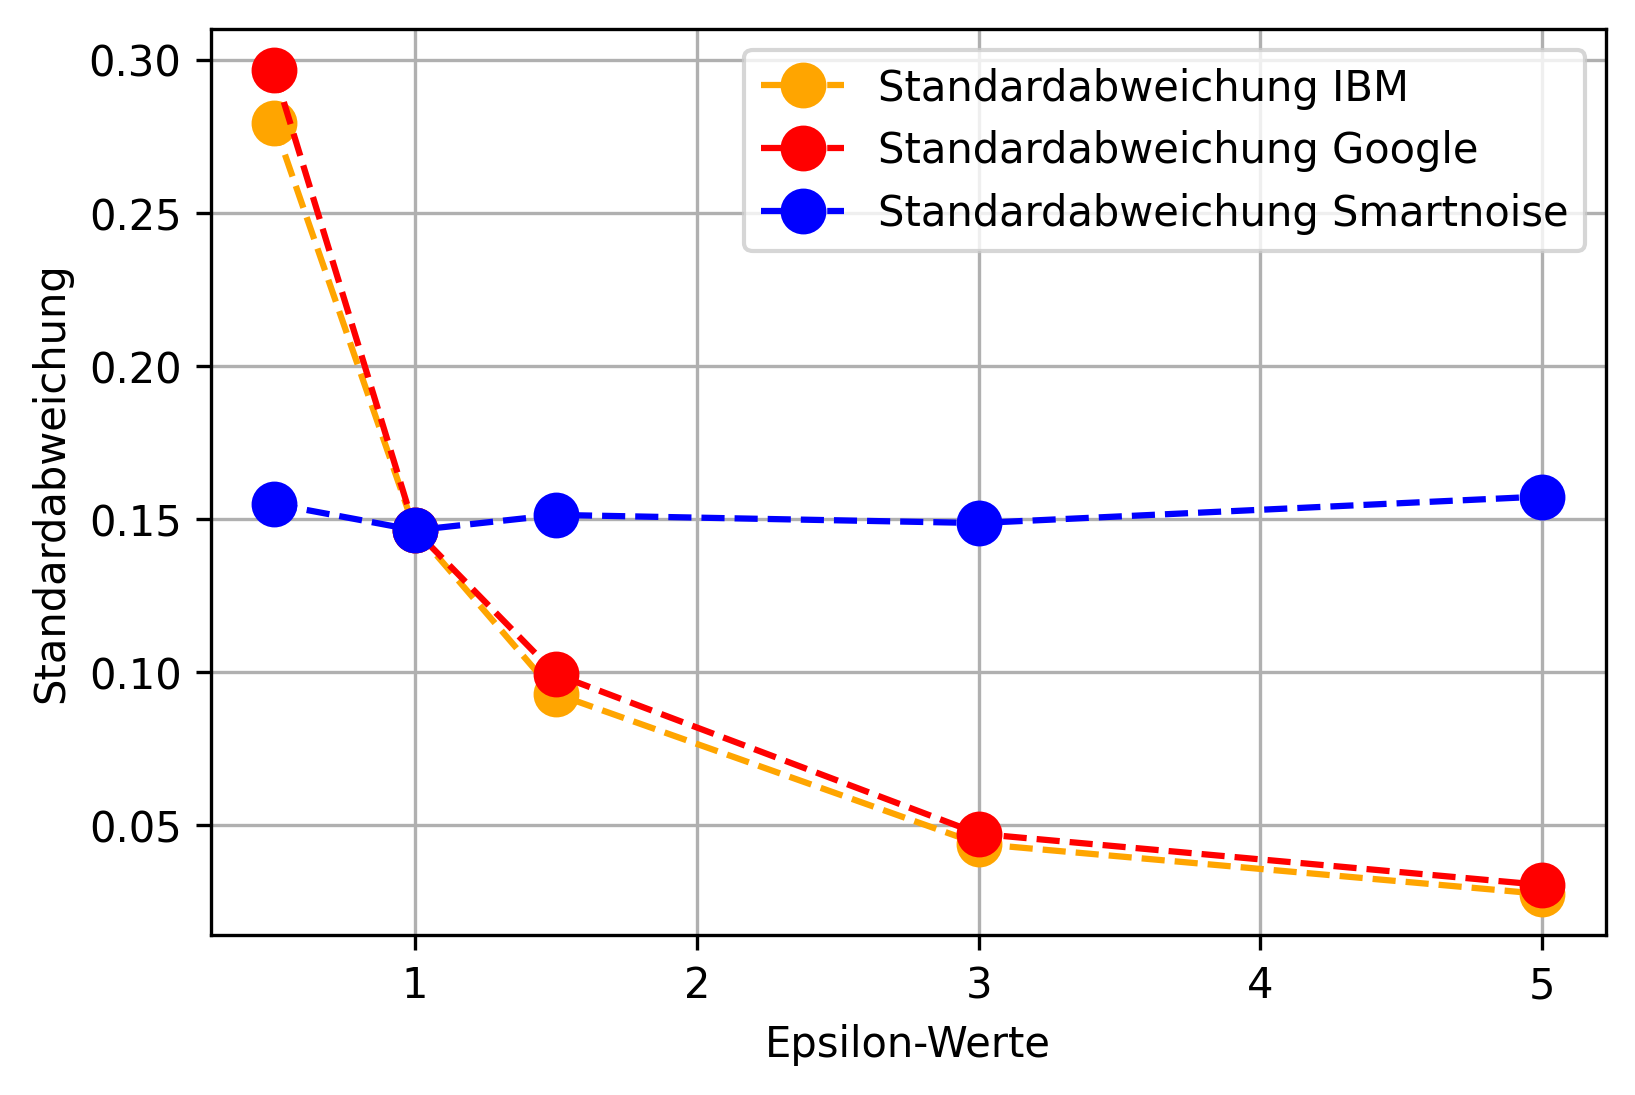
\includegraphics[scale=0.6]{./images/together_std.png}
	\caption{Die Gesamtübersicht der drei Frameworks in der Metrik Standardabweichung.}
	\label{fig:together_std}
\end{figure}

\textbf{Vergleich: }
Im Ergebnis zeichnen sich deutliche Muster wie in \cref{fig:together_std} ab. IBM \gls{dp} sowie Google \gls{dp} verlaufen nahe zu parallel, da beide mit steigendem $\epsilon$-Wert weniger Verrauschen zu den Daten hinzufügen. Die verrauschten Ausgaben weichen weniger ab, sodass die Genauigkeit zunimmt. Die minimale Genauigkeit ist am ersten Punkt und die maximale Genauigkeit am letzten Punkt vorhanden. In Kontrast dazu steht die Kurve von Smartnoise SDK. Sie stagniert über die verschiedenen $\epsilon$-Werte hinweg und verliert keineswegs an Genauigkeit. Der Mechanismus beim Smartnoise SDK hat eine konstante Abweichung in seiner verrauschten Ausgabe, weswegen die erwartete höhere Genauigkeit in den größeren $\epsilon$-Werten verloren geht. 

\newpage
\section{Erwartungstreue}
In diesem Abschnitt wird die Verzerrung der verrauschten Daten betrachtet. Inwieweit sie von den unveränderten Daten abweichen. Diese Auswirkungen betreffen die Semantik der Daten.
\subsection{Mittlere vorzeichenbehaftete Abweichung}
Mit dieser Metrik wird gefolgert, ob das Verrauschen die Semantik des unveränderten Datensatzes bewahrt und ob im Durchschnitt zu wenig oder zu viel hinzugerechnet wurde. Dafür war die Eingabe zum einen der erste verrauschte Datensatz und zum anderen der unveränderte Datensatz.
\begin{figure}[htbp]
	\centering
	\subfloat[Das Ergebnis von IBM \gls{dp} für die Standardabweichung.]{
		\label {fig:ibm_msd}
		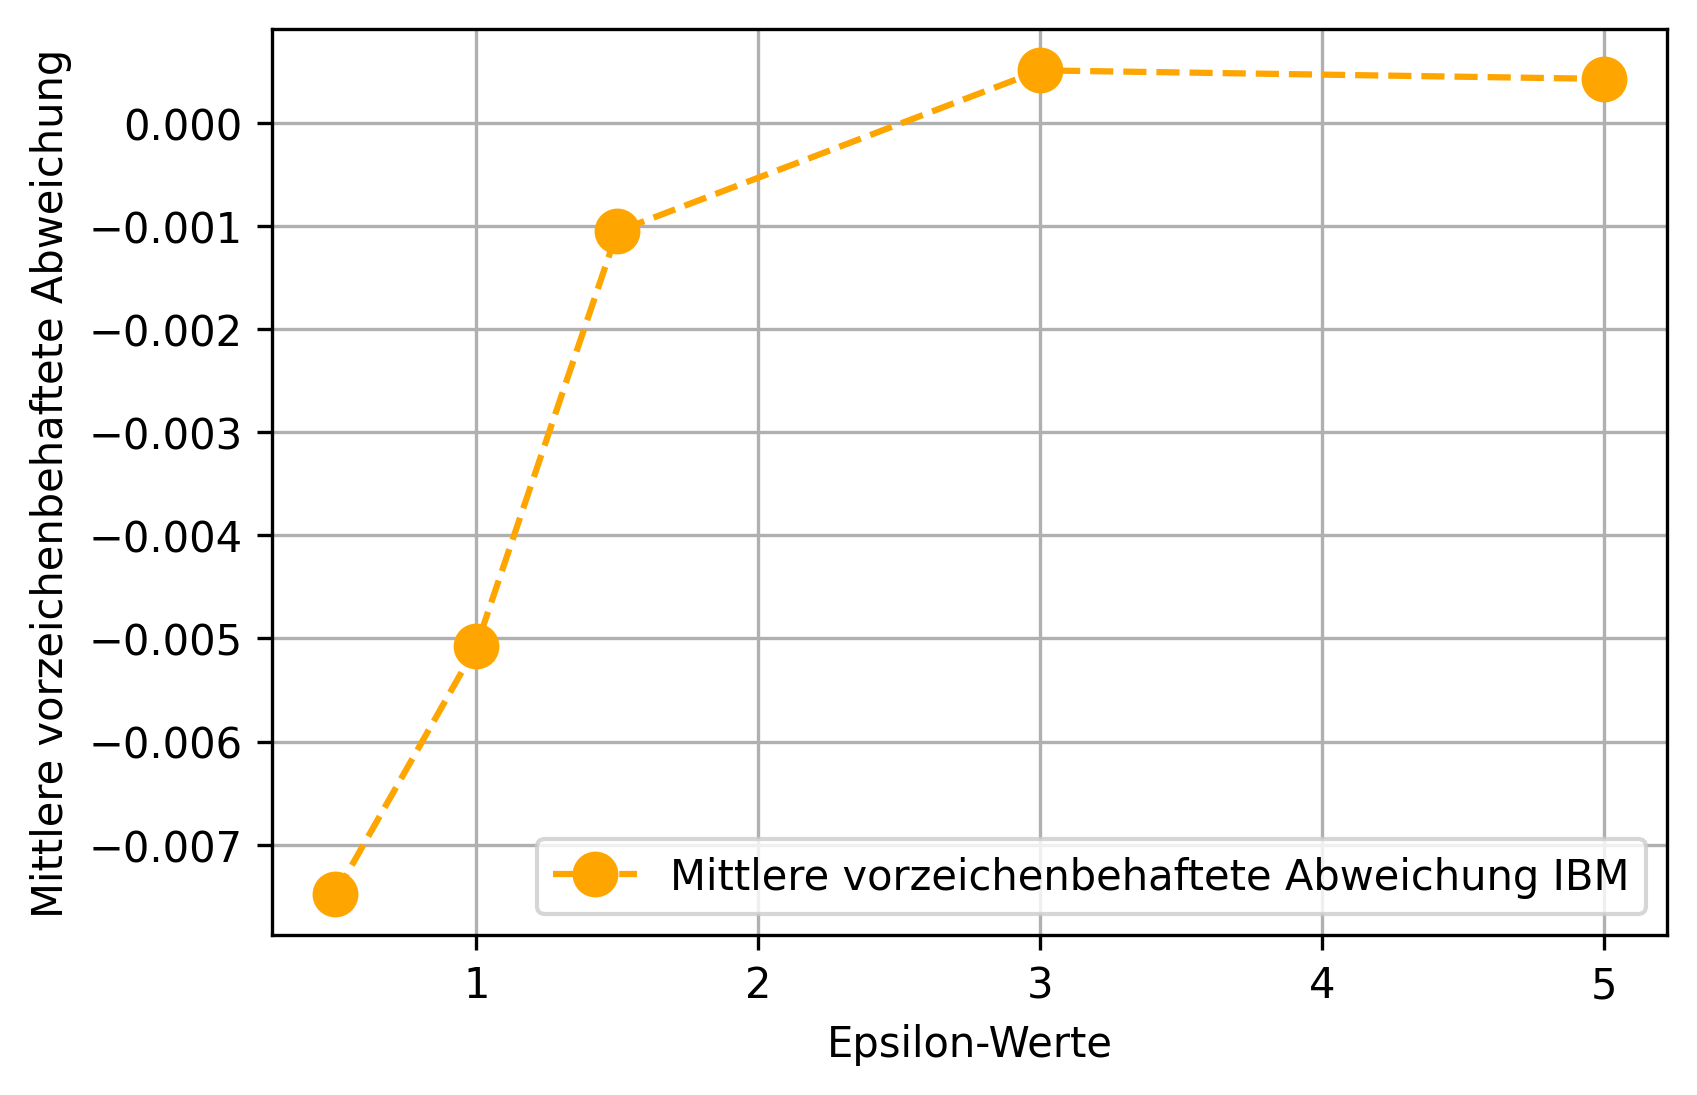
\includegraphics[scale=0.4]{./images/ibm_msd.png}
	} \qquad
	\subfloat[Das Ergebnis von Google für die Standardabweichung.]{
		\label {fig:google_msd}
		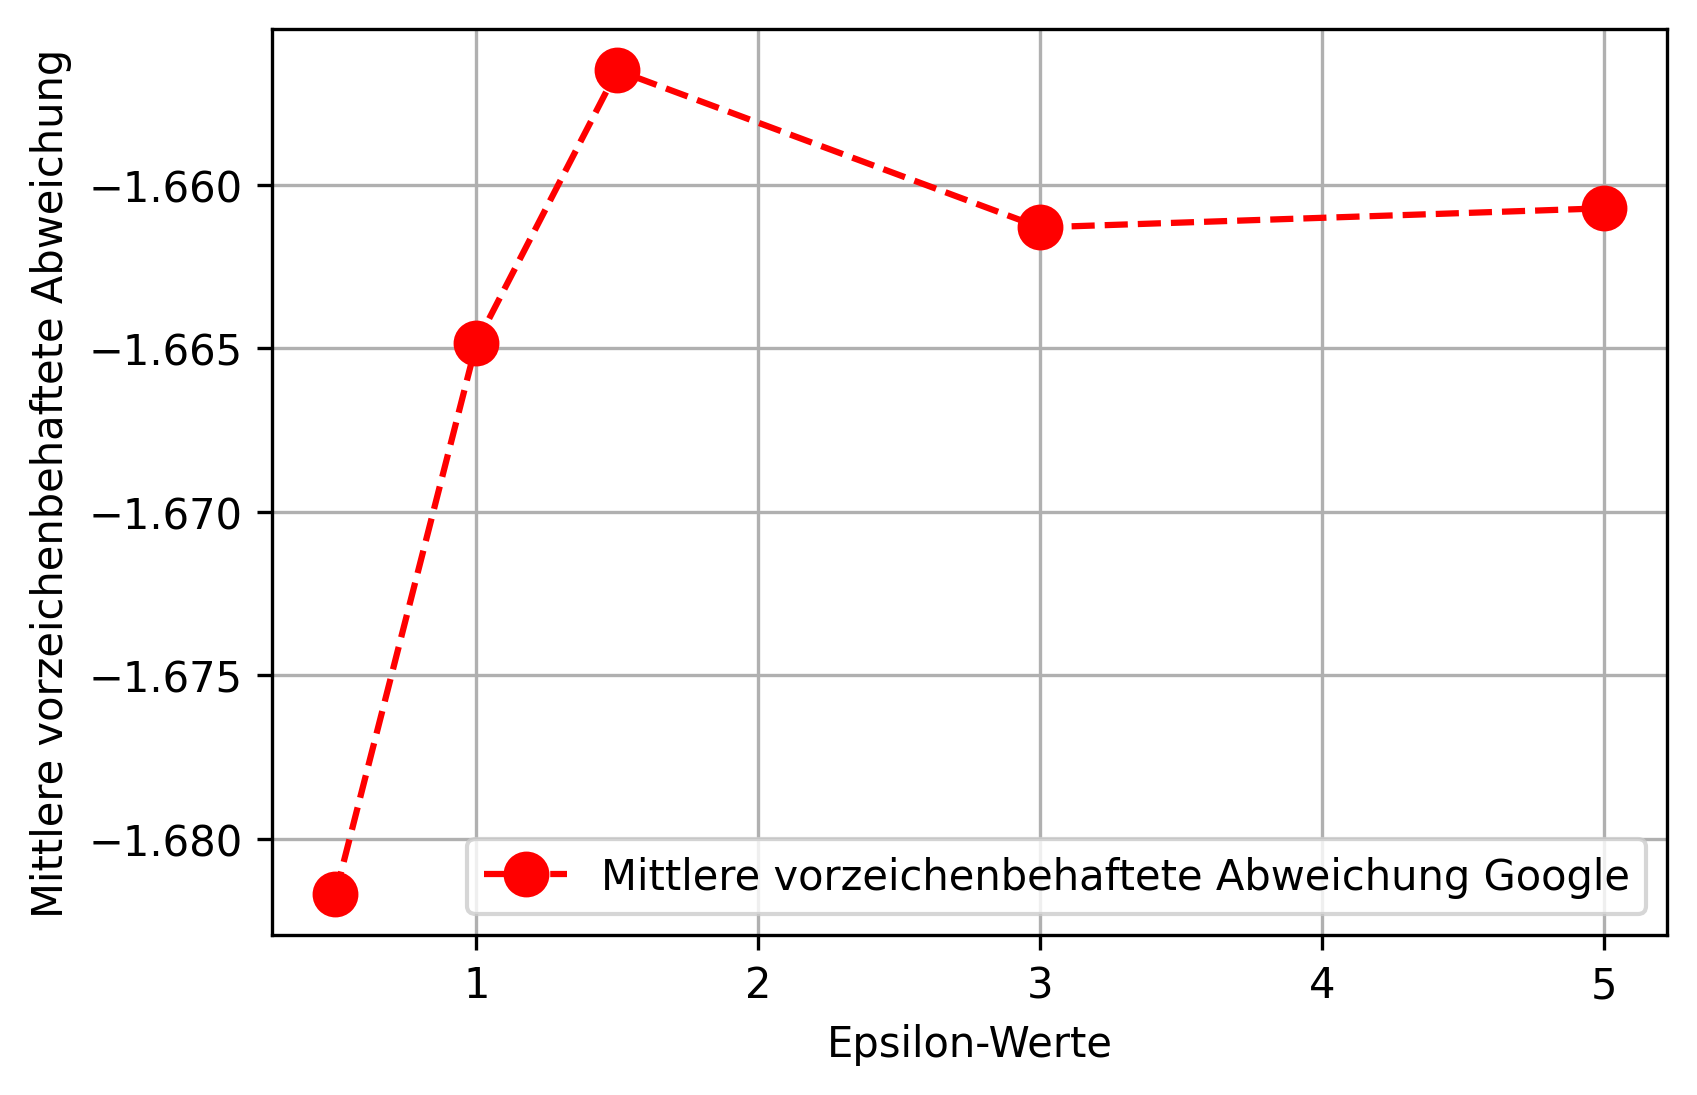
\includegraphics[scale=0.4]{./images/google_msd.png}
	}
	\subfloat[Das Ergebnis von Smartnoise SDK für die Standardabweichung.]{
		\label {fig:sn_msd}
		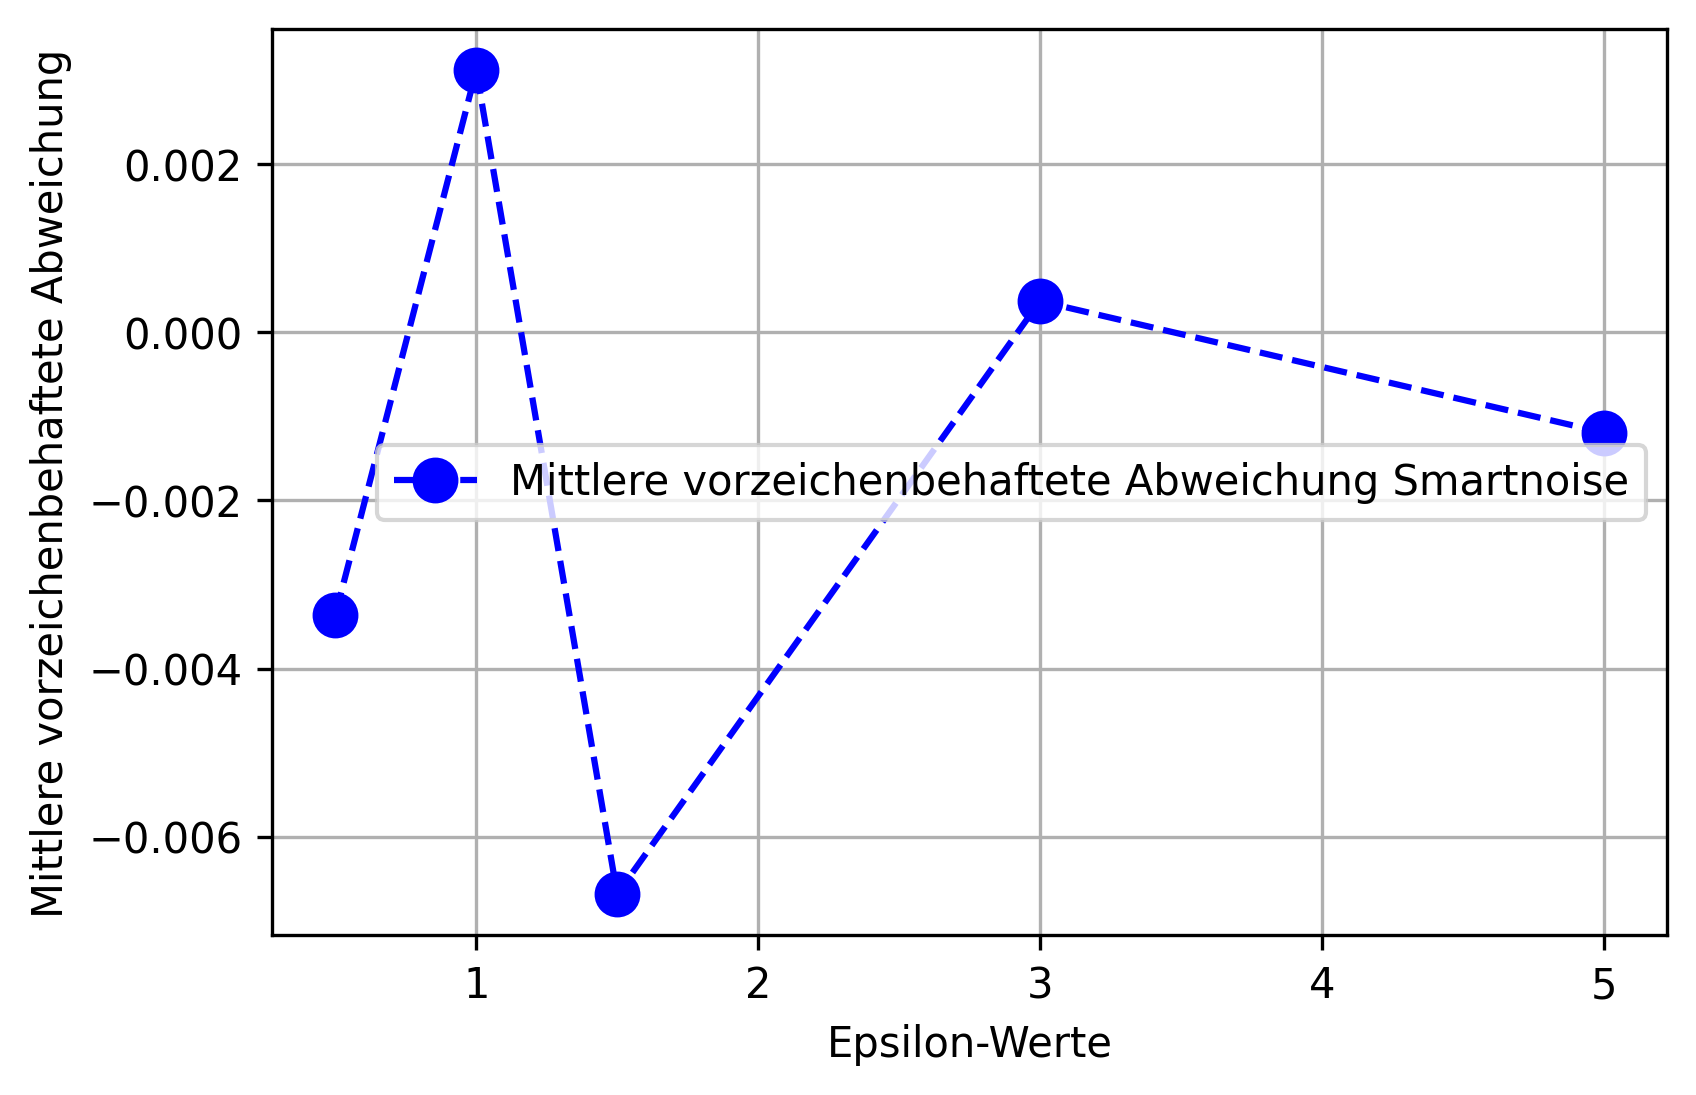
\includegraphics[scale=0.4]{./images/sn_msd.png}
	}
	\caption{Die Ergebnisse der Standardabweichung für die $\epsilon$-Werte [0,5;1,0;1,5;3,0;5,0] der drei Frameworks.}
	\label{fig:msd}
\end{figure}

\textbf{Erwartetes Ergebnis:}
Nach dem Laplace Mechanismus hat die Laplace Verteilung den Erwartungswert $\mu$=$0$. Dadurch soll die Aussagekraft der verrauschten Daten beibehalten werden. Bei kleinen $\epsilon$-Werten ist ein höherer Wert der Metrik zu erwarten,  da dann die Privatsphäre mehr geschützt wird und das Verrauschen verstärkt ist. Das Vorzeichen spielt in erster Rolle keine essentielle Rolle, sondern der Betrag des Wertes. Es kann insoweit ein typisches Verhalten des Mechanismus nach zeigen, ob grundsätzlich zu viel oder zu wenig hinzugefügt worden ist.

\textbf{IBM \gls{dp} Ergebnis:}
Die Kurve in \cref{fig:ibm_msd} verläuft mit steigendem $\epsilon$ streng monoton steigend gegen den Wert $0$, sodass die Verzerrung stets abnimmt. Die semantische Nutzbarkeit der Daten bleibt erhalten. Im Gesamtüberblick der Werte liegen sie bei fast $0$, wodurch ein Verlust der semantischen Aussagekraft  nicht einhergeht.

\textbf{Google Ergebnis:}
In den Zwischenergebnissen sinkt der Wert des Durchschnitts durch das Verrauschen des Mechanismus auf 34. In \cref{fig:google_msd} folgt die Konsequenz durch diese Metrik, welche sehr groß und ausschließlich negativ ausgefallen ist. Dies zeigt ein Muster des Mechanismus auf. Eine höhere Verzerrung liegt bei den ersten zwei Punkten wie erwartet vor, jedoch der dritte Punkt ist ein Ausreißer, wogegen die letzten zwei Punkte stagnieren. Die semantische Bedeutung ist bei den letzten zwei Punkten konstant gehalten, wogegen sie zu vor abnimmt. Insgesamt folgt bei der Auswertung ein hoher semantischer Verlust der verrauschten Daten, somit ebenfalls an Nutzbarkeit.

\textbf{Smartnoise SDK Ergebnis:}
Die Werte der Metrik liegen in \cref{fig:sn_msd} sehr nahe an $0$. Ein Verschwinden der semantischen Bedeutung der verrauschten Datensätze geht nicht hervor. Die Verteilung der Punkte in der Abbildung sind verstreut, sodass kein konstantes Verhalten des Mechanismus hervorgeht. Grundsätzlich gilt bei kleinen $\epsilon$-Werten betragsmäßig ein höherer Wert als bei großen, damit die Verzerrung die Nachvollziehbarkeit der unveränderten Daten erschwert (Schutz der Privatsphäre). Hier wird dies nicht eingehalten.
\begin{figure}[htbp]
	\centering
	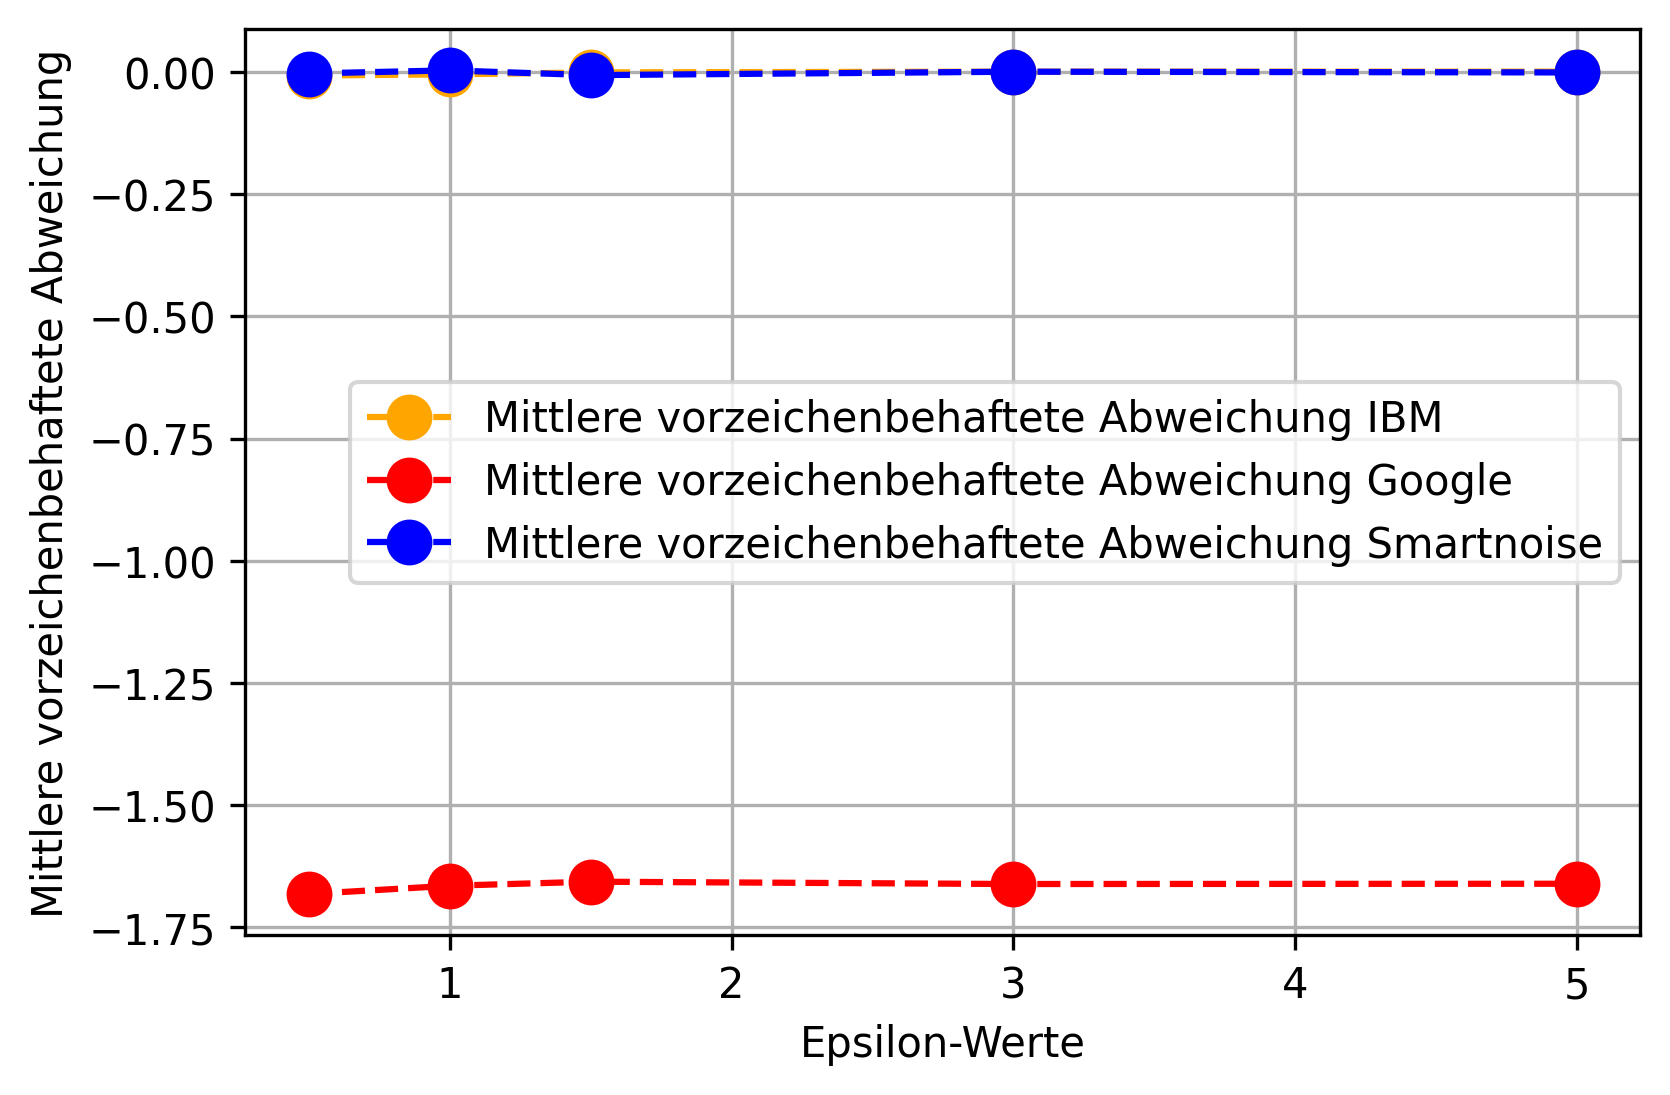
\includegraphics[scale=0.6]{./images/together_msd.png}
	\caption{Die Gesamtübersicht der drei Frameworks in der Metrik Mittlere vorzeichenbehaftete Abweichung.}
	\label{fig:together_msd}
\end{figure}

\textbf{Vergleich: }
Die beiden Frameworks Smartnoise SDK sowie IBM \gls{dp} bewahren die Nutzbarkeit der verrauschten Datensätze auf einem Niveau wie in \cref{fig:together_msd} erkennbar. Dies erlaubt den verrauschten Datensätze eine hohe Aussagekraft zu behalten. In Verhältnis dazu verzerrt Google durchschnittlich die Werte sehr durch zu viel negatives Rauschen. Damit geht ein großer Verlust der Semantik der Daten einher. In den Zwischenergebnissen liegen daher die verrauschten Werte bei den erstgenannten Frameworks bei ca. 36, wogegen bei Google stets um den Wert 34.
\newpage
\section{Performance}
In diesem Kapitel wird die Performance der Berechnung von verrauschten Werten evaluiert. Die Berechnung sind die 10,000 verrauschten Durchschnittswerte, die aus den 5 $\epsilon$-Werten mit jeweils 1,000 Durchführungen für zwei Datensätze resultieren. Die Anzahl an Iterationen für IBM \gls{dp} und Google \gls{dp} beträgt 1,000 und beim Smartnoise SDK 100.

\subsubsection{Bedingungen}
Zunächst erfolgt die Messung der Ausführungszeit ausschließlich der zuvor genannten Berechnung. Es werden keine Overheads wie die Verbindung, Einlesung oder Verarbeitung der Daten usw. berücksichtigt. Die Relevanz liegt auf der verrauschten Funktion durch das Framework.

Im Gegensatz dazu wurde Google \gls{dp} in der Programmiersprache Java genutzt. Eine Verlagerung der Berechnung auf den Server war aufgrund von serverseitigen Einstellungen zu aufwendig, weswegen sie lokal durchgeführt wurde. Trotz dessen ist dies nicht von belangen, denn die Ausführungszeit ist lokal sehr kurz. Somit wird hierbei schon ein Trend des Frameworks klar ersichtlich.

\subsubsection{Ausführungszeiten der Frameworks}
\begin{figure}[htbp]
	\centering
	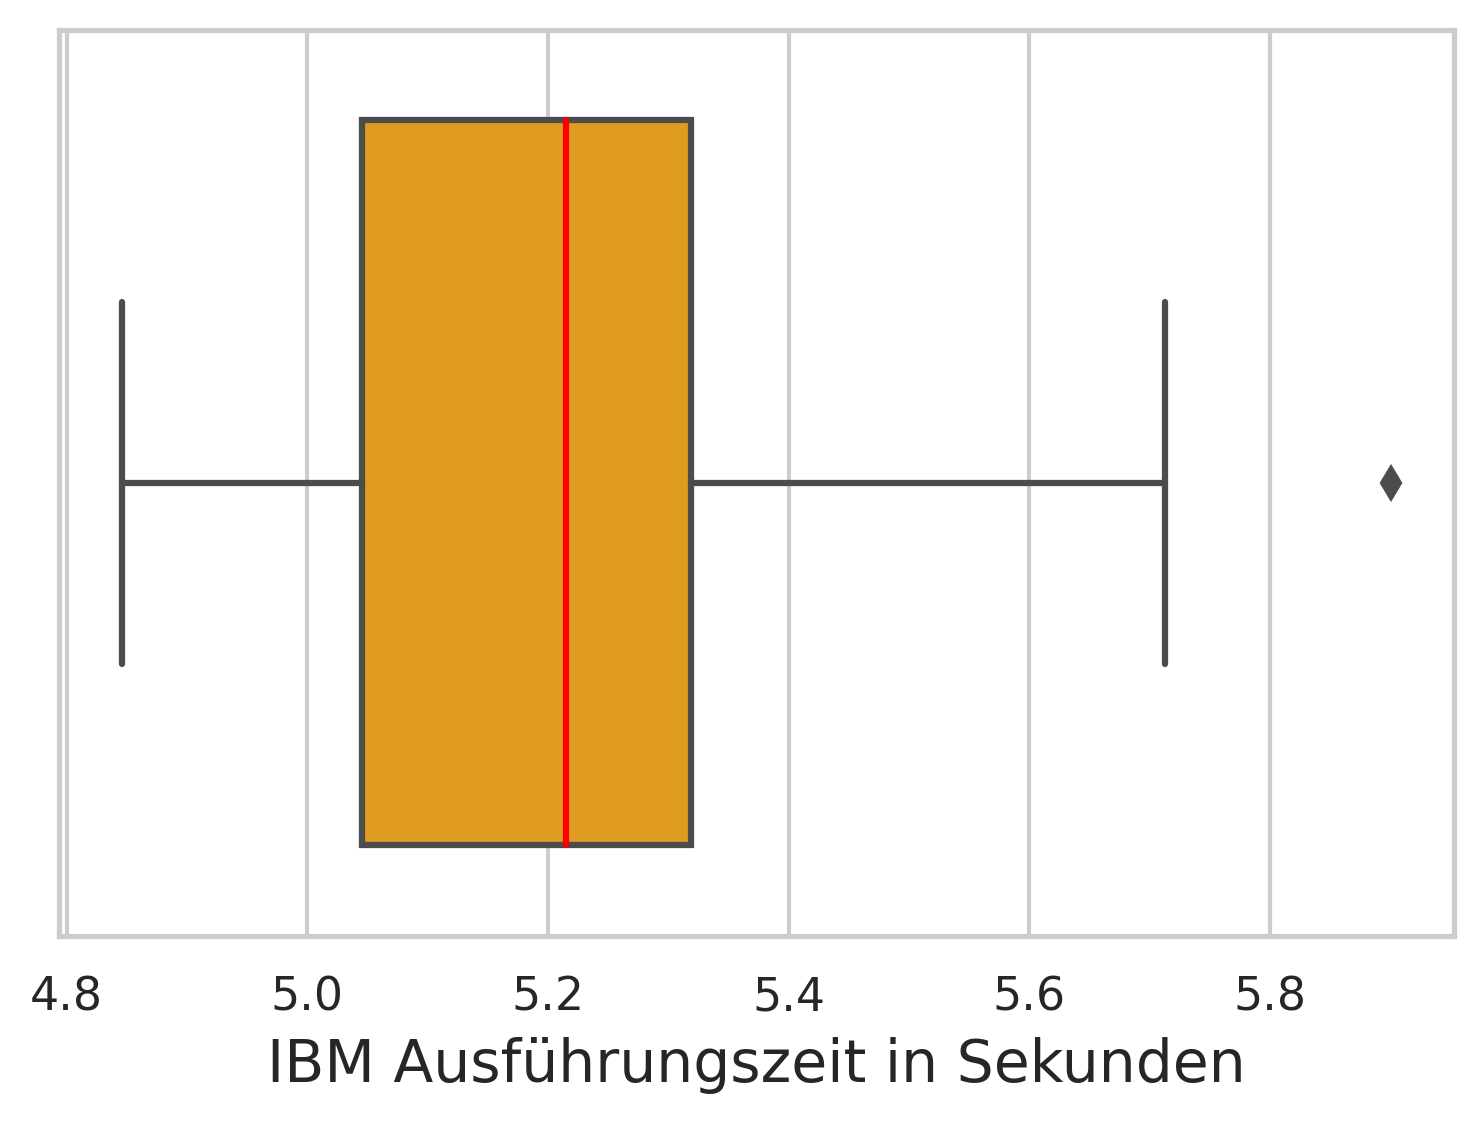
\includegraphics[scale=0.6]{./images/boxplot_ibm.png}
	\caption{Die Ausführungszeit von IBM \gls{dp} für die Berechnung der verrauschten Durchschnittswerte (10,000 Werte).}
	\label{fig:boxplot_ibm}
\end{figure}
\textbf{Ergebnis von IBM \gls{dp}:}
In \cref{fig:boxplot_ibm} ist der Boxplot der Ausführungszeiten von IBM \gls{dp} dargestellt. Der Median für die Zeit liegt bei 5,2 Sekunden. 50 \% der Iterationen weisen eine Zeit zwischen 5.05 und 5,32 Sekunden auf. Im unteren Viertel liegen die Werte zwischen 4.85 und 5.05 Sekunden und im oberen Viertel zwischen 5,32 und 5,71 Sekunden. Im Gesamten gibt es nur einen einzigen Ausreißer mit der Ausführungszeit 5,90. Insgesamt verläuft die Ausführungszeit schnell und stabil. Damit kann es mit hoher Nutzbarkeit angewendet werden.

\begin{figure}[htbp]
	\centering
	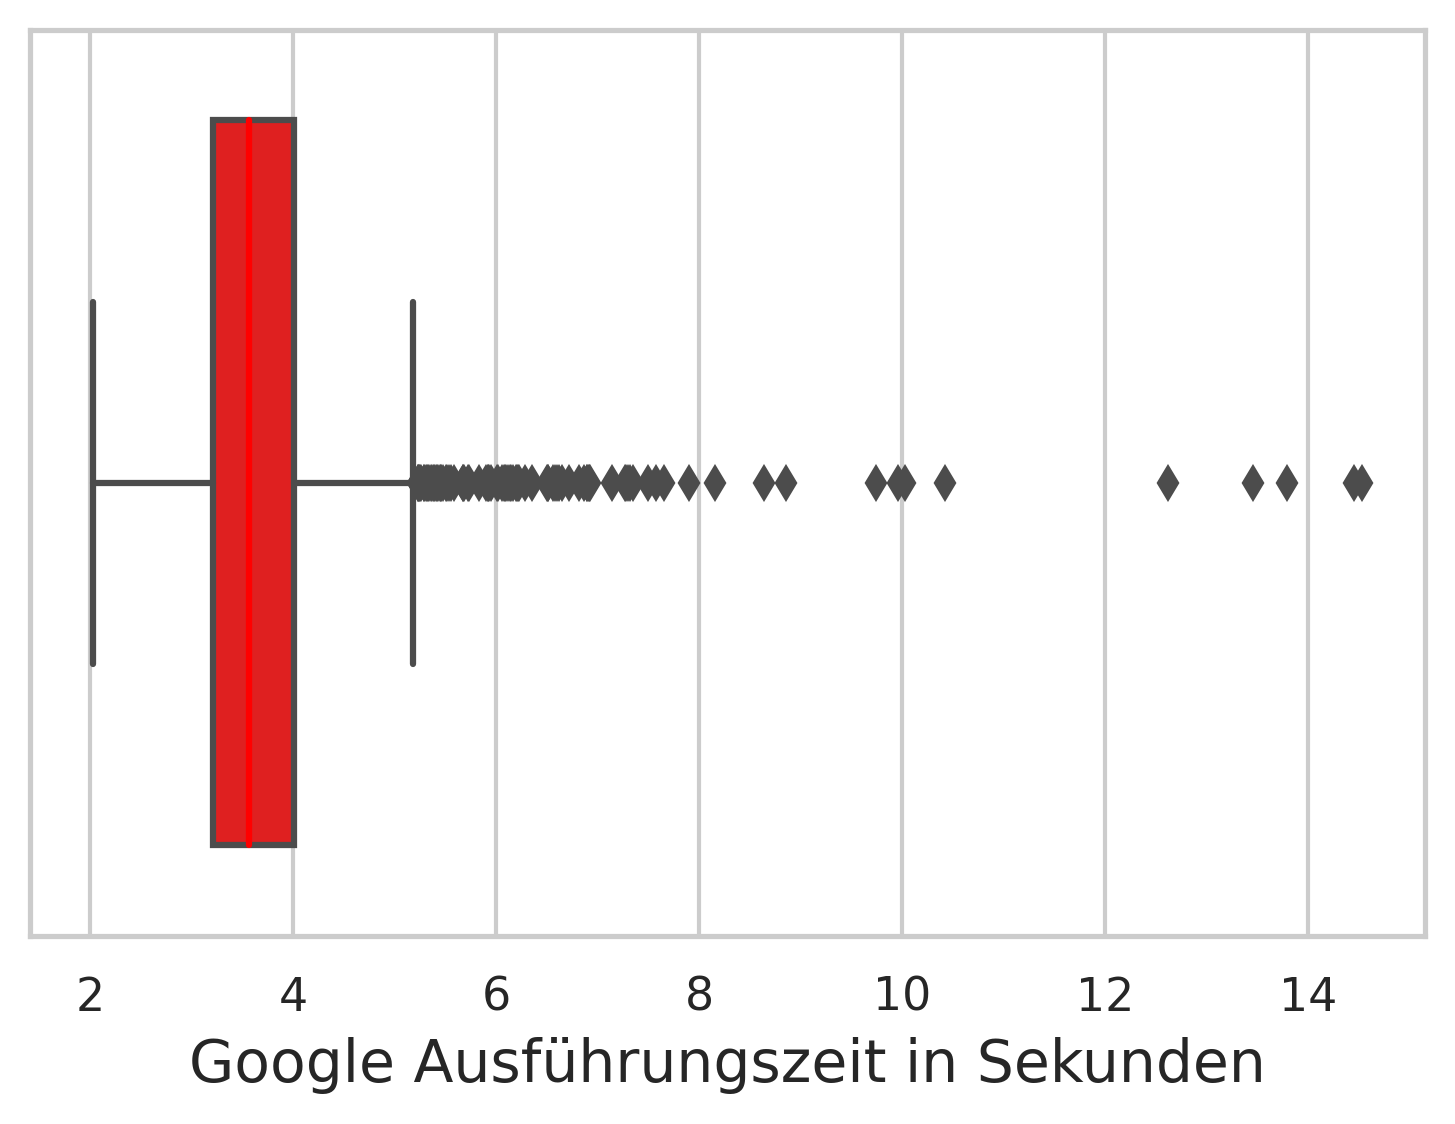
\includegraphics[scale=0.6]{./images/boxplot_google.png}
	\caption{Die Ausführungszeit von Google für die Berechnung der verrauschten Durchschnittswerte (10,000 Werte).}
	\label{fig:boxplot_google}
\end{figure}

\textbf{Ergebnis von Google:}
In \cref{fig:boxplot_google} ist der Boxplot der Ausführungszeiten von Google dargestellt. Der Median liegt bei 3,6 Sekunden, welcher eine schnelle Ausführungszeit aufzeigt. 50 \% der Iterationen weisen eine Zeit zwischen 3,21 und 4,01 Sekunden auf. Im unteren Viertel liegen die Werte zwischen 2,03 und 3,21 Sekunden und im oberen Viertel zwischen 4,01 und 5,18 Sekunden. Die Anzahl an Ausreißer beträgt 93 und betrifft 9,3 \% der Ausführungen. Dies weist eine gewisse Instabilität auf, die jeden 10. Durchlauf betrifft. Hierbei liegt das Maximum bei 14,53 Sekunden, wobei einige Ausreißer wie 14,45 Sekunden, 13,79 Sekunden und 12,62 Sekunden in die Nähe dessen liegen. Das Minimum liegt bei 2,03 und weißt unterdessen keine Ausreißer auf. Die Ursache für das vermehrte Auftreten von Ausreißern ist nicht erklärbar und auf das Framework zurückzuführen.

\textbf{Ergebnis von Smartnoise SDK:}
Bei Smartnoise SDK beansprucht die Ausführungszeit ca. 2 Stunden, weswegen eine Evaluation von 1000 Iterationen im Rahmen der Arbeit nicht umsetzbar gewesen ist. Aufgrund dessen beträgt die Anzahl für die Iteration 100, trotz dessen ein klares Muster der Laufzeit sich abzeichnet.

In \cref{fig:boxplot_sn} wird die lange Ausführungszeit deutlich. Der Median liegt hierbei bei 1,98 Stunden, also fast 2 Stunden. Ca. 25 \% der Ausführungszeiten liegen über 2 Stunden. Die Spanne dabei beträgt zwischen 2,03 und 2,19 Stunden. Der untere Quantil umfasst die Werte zwischen 1,75 und 1,89 Stunden. Insgesamt sind keine Ausreißer vorgekommen.
\begin{figure}[p]
	\centering
	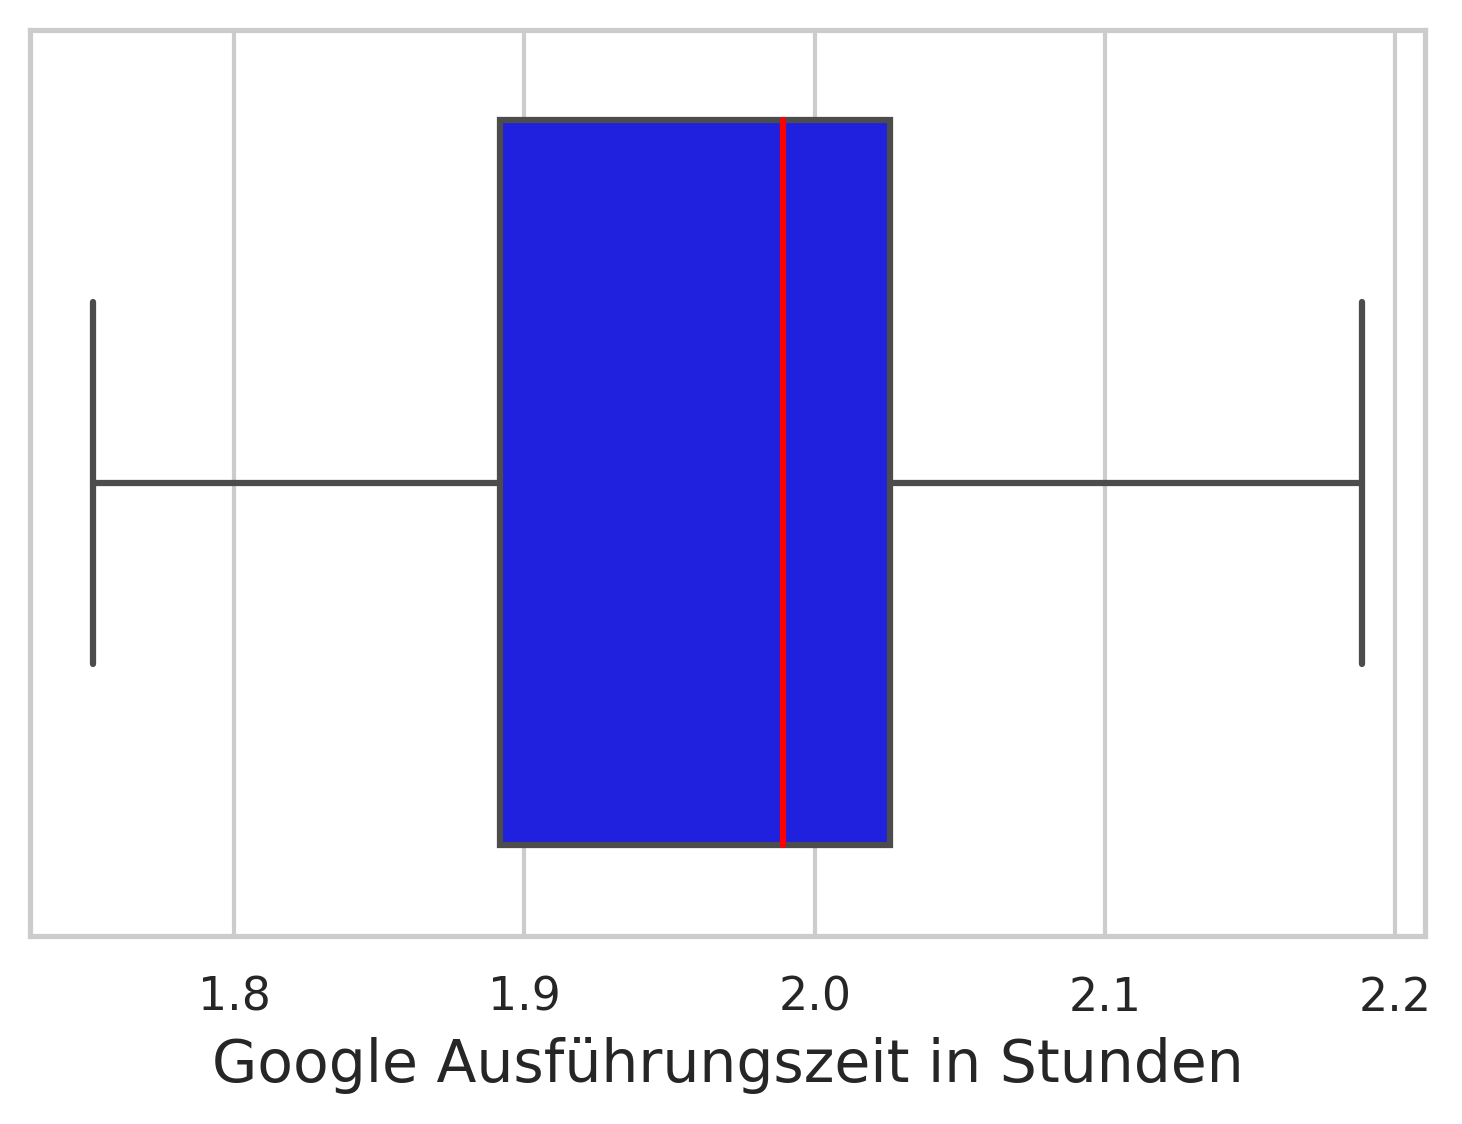
\includegraphics[scale=0.6]{./images/boxplot_sn.png}
	\caption{Die Ausführungszeit von Smartnoise SDK für die Berechnung der verrauschten Durchschnittswerte (10,000 Werte).}
	\label{fig:boxplot_sn}
	\vspace{100in}
\end{figure}

\chapter{Folgerungen}
In der vorliegenden Bachelorarbeit wurden die drei Frameworks IBM DP, Google DP und Smartnoise SDK in einem medizinischen Anwendungsfall evaluiert. Hierfür wurde eine generische Schnittstelle programmiert. Sie liest medizinische Alterswerte von mit COVID-19 infizierten Personen ein und berechnet ihren Durchschnittswert durch die entsprechende \gls{dp} Funktion der Frameworks. Anhand von Metriken werden die verrauschten Durchschnittswerte auf Privatsphäre, Genauigkeit und Erwartungstreue bewertet.

Die ausgeführte Evaluation zeigt deutlich auf, dass IBM DP in allen Kategorien stets insgesamt die besten Werte bei den Metriken erzielt hat. Hierauf folgend liegt das Framework Smartnoise SDK, welches durchschnittliche instabile Qualität in den metrischen Werten erreicht hat. Dagegen hat das Google DP Framework in allen bis auf die Metrik Standardabweichung geringe Leistung in den Metriken aufgezeigt. In der Ausführungszeit liegen IBM DP und Google DP im Sekundenbereich, erheblich entgegengesetzt liegt Smartnoise SDK im Stundenbereich. Im vorgestellten medizinischen Anwendungsfall ist IBM \gls{dp} ohne Einschränkungen einsetzbar, jedoch Smartnoise SDK aufgrund von zeitlichen Einschränkungen nicht verwendbar ist.
\section{Einsetzbarkeit}
Bei der Einsetzung eines der drei Frameworks ist zu beachten, dass Analysten in Kenntnis der Grundkonzepte von \gls{dp} sein sollten. Bei der Verwendung des Frameworks können unerwartete und widersprüchliche Resultate auftreten, die auf das Framework zurückzuführen sind. In der Evaluation dieser Bachelorarbeit wurden Mehrfachdurchführungen zur Berechnung der Metriken ausgeführt, um gewisse Muster zu erkennen und die richtigen Ergebnisse auszusortieren. Denn bei allen Frameworks kamen in manchen Metriken wie die Wasserstein-Distanz unerwartetes Verhalten auf. Somit folgen durch Analysen keine eindeutigen Ergebnisse, sondern welche mit Fehlertoleranzen.

Vor der praktischen Nutzen eines der Frameworks muss die Verbindung zum zentralen Server aufgestellt werden. Wie bereits in Kapitel 4 erwähnt, hat Smartnoise SDK als einzige die Möglichkeit eine unmittelbare Verbindung zu einer Datenbank herzustellen. Die anderen bräuchten eine zusätzliche Verbindung, um nicht auf die Rohdaten zugreifen zu müssen. Des Weiteren muss das \gls{pb} serverseitig reguliert und anpassbar sein. Der Forscher will entsprechend seiner Daten die Privatsphäre beliebig stark schützen. Bei sensiblen Attributen sowie bei Quasi-Identifikatoren, die selbst keine Identifikatoren sind, allerdings in Kombination mit Hintergrundwissen eine eindeutige Zuordnung ermöglichen, sind kleinere $\epsilon$-Werte erforderlich. Der Server muss in der Lage sein ebenfalls mit kleinen $\epsilon$ arbeiten zu können.

Eines der wichtigsten Aspekte für die Einsetzung eines der Frameworks ist die Ausführungszeit bei Anfragen. Ein Forscher stellt mehrere verschiedene Anfragen, um gewisse Erkenntnisse oder Strukturen über die Ergebnisse zu erfahren. Vor allem bei medizinischen Daten sind die Anzahl an Einträge sehr groß und vielfältig. In der Evaluation sind die Resultate zu den Ausführungszeiten der Frameworks eindeutig. IBM \gls{dp} und Google \gls{dp} können 10,000 Werte in wenigen Sekunden berechnen, wogegen Smartnoise SDK dafür ca. 2 Stunden benötigt wie in \cref{tab : classification} dargestellt. Auf dem genannten Server ist ebenfalls aufgefallen, dass die Berechnungen von Smartnoise SDK sehr viel Speicher verbraucht. Die wohl mögliche Ursache geht auf die Struktur des Frameworks zurück. Wenn eine Berechnung durchgeführt werden soll, dann ist eine SQL-Abfrage erforderlich. Zunächst wird sie in Python angegeben und durch interne Strukturen wie der Parser interpretiert und in Python ausgeführt. Dies kann zu einem großen Overhead bei der Berechnung führen und eine Erklärung für den großen Speicherverbrauch sein. Daher eignet sich selbst Smartnoise SDK auf einem Server nicht für Mehrfachanwendungen von Funktionen oder aufwendige Berechnungen.

In dieser Evaluation ist eine \gls{dp} Funktion durchgeführt worden, um weitere Erkenntnisse über die Anwendbarkeit der Frameworks im medizinischen Forschungsalltag zu erhalten, sollten weitere Funktionen folgen. Zunächst mit einfachen Funktionen wie die Summe, die Anzahl etc. und steigend Komplexere wie Laplace Mechanismen für verrauschte Einzelwerte evaluiert werden. Dies soll Aufschluss vor allem über die Ausführungszeit der Anfragen ergeben, um das Framework Smartnoise SDK doch noch einsetzen zu können.  

\section{Schutz und Nutzbarkeit der Daten}
\begin{table}[h]
	\centering
	\begin{tabular}{ l l l l} \toprule
		\textbf{Metrik} & \textbf{IBM DP} & \textbf{Google DP} & \textbf{Smartnoise SDK}  \\ \midrule
		\textit{Privatsphäre:}&&&\\ \hline
		\textit{DP-res}	& $\checkmark$ &$\checkmark$ &$\checkmark$ \\ 
		\textit{WD}	& Hoch  & Niedrig & Mittel \\
		\textit{Genauigkeit:}&&&\\ \hline
		\textit{MSE}	& Hoch & Niedrig & Hoch\\
		\textit{STD}	&  Hoch& Hoch & Mittel\\
		\textit{Erwartungstreue:}&&&\\ \hline
		\textit{MSD}	&  Hoch & Niedrig & Hoch\\ 
		\textit{Performance:}&&&\\ \hline
		\textit{Ausführungszeit}	&  Sekundenbereich & Sekundenbereich & Stundenbereich\\ \bottomrule
	\end{tabular}
	\caption{Die Einstufung der Frameworks in den Metriken aus der Evaluation.}
	\label{tab : classification}
\end{table}

In medizinischen Statistiken aus Rohdaten werden verschiedene Aspekte berücksichtigt, die anhand der Ergebnisse aus der Evaluation in \cref{tab : classification} über die Einsetzbarkeit der Frameworks Aufschluss geben soll.

Die Hauptpriorität ist stets bei Veröffentlichung von medizinischen Daten die Privatsphäre des einzelnen Patienten entsprechend der Verordnung der \gls{dsgvo}. Durch die Definition von \gls{dp} soll ein einzelner Eintrag in einer Datenmenge bis zu einem messbaren Risiko geschützt werden. Hierfür dient die Metrik DP-res, welche die Ausgabe der Frameworks mit der DP Definition validiert. Aus den Ergebnissen in \cref{tab : classification} geht hervor, dass die Ausgabe jedes Framework dies erfüllt. Ausschließlich mit dieser Erfüllung dürfen die verrauschten Daten für die medizinische Forschung genutzt werden, somit dient dies als Bedingung. Dies ist jedoch verständlich, da jedes Framework speziell für die Einhaltung von der Definition von \gls{dp} konstruiert worden ist.

In der medizinischen Forschung handelt es sich stets um sensible Daten. Manche von ihnen sind schützenswerter aufgrund ihres großen Personenbezuges. Ein gewisser Grad an Sensibilität der Daten ist vorhanden. Entsprechend diesem handelt das \gls{pb}, womit die Stärke des Schutzes der Privatsphäre reguliert werden kann. Die Qualität des Schutzes der Privatsphäre ist unterschiedlich bei den Frameworks wie in \cref{tab : classification} ersichtlich ausgefallen. Google DP hat für den kleinsten $\epsilon$-Wert sehr gut abgeschnitten, jedoch bei den restlichen sind niedrige Werte aufgetreten. Für eine medizinische Veröffentlichung kann der Schutz zu niedrig sein und zu Re-Identifizierung von Patienten führen. Smartnoise SDK leidet an Schwankungen bei kleinen $\epsilon$-Werten, was zu einer Instabilität des Schutzes führt. Vor allem für sensible Daten ist ein erwünschter hoher Schutz dadurch nicht garantiert. Insgesamt ist eine recht hoher mit relativer Instabilität an Schutz dargeboten. Schlussendlich garantiert IBM DP den Forschern ein Verhalten entsprechend ihrer Erwartungen. Ein durchgehender hoher Schutz der Privatsphäre ist vorhanden und es weist keine Instabilität bei der Ausgabe auf.

Eine ursprünglicher Gedanke ist, wenn die Privatsphäre gut geschützt ist, dann ist die Ungenauigkeit verstärkt vorhanden. Dies gilt nicht beim Smartnoise SDK und vor allem beim IBM \gls{dp}. Sie erreichen bei der Metrik MSE sehr kleine Werte, was für eine sehr geringe Abweichung vom originalen Durchschnitt der Rohdaten sorgt. Für die Statistik der medizinischen Daten werden dadurch die Aussagekraft und semantische Richtigkeit erlangt. Hingegen beim Google DP ist der Mechanismus für den schlechten Ausfall der Metrik MSE zuständig. Des Weiteren folgen bei Forschungen mehrfache Anfragen für dieselbe Thematik, dies bedeutet im Framework die mehrfache Ausführung von \gls{dp} Funktionen. Ein Forscher muss auf die Stabilität des Frameworks vertrauen können, damit die Streuung der Verrauschens nicht erheblich abhängig von der Anzahl an Anfragen ist. Diesen Aspekt deckt die Metrik STD, welche bei IBM DP und Google nahezu identisch ausfallen, ab. Smartnoise SDK stagniert bei diesem Wert, sodass die Ausgabe bei mehrfacher Anfrage minimal verändert wird. Diese Stagnation kann für kleine $\epsilon$-Werte zu geringen Schwankungen bei der Ausgabe durch das Verrauschen führen. Für die Aussagekraft von Statistiken und Forschungen ist die Genauigkeit der Daten unentbehrlich, in diesem Rahmen erfüllt IBM DP dies mit hoher Leistung, wobei Google DP große Ungenauigkeit nachweist. Dazwischen liegt das Framework Smartnoise SDK.

Nach dem theoretischen Aspekt dieser Frameworks basieren sie alle auf dem Laplace Mechanismus mit einem Erwartungswert von $0$, wodurch er im Durchschnitt mit den Rohdaten übereinstimmen soll. Bei dem Parameter $b$ für den Mechanismus bestimmt das Verhältnis zwischen der Sensitivität und dem $\epsilon$-Wert. Die Erwartungstreue der Frameworks sollte nach der Theorie vorhanden sein, da ihre Laplace Verteilung, worauf das Verrauschen basiert, zentriert ist. Damit bleibt vor allem die semantische Bedeutung der Daten durch das Verrauschen erhalten. In Forschungen werden basierend auf Daten Erkenntnisse vollzogen, die auf einem Fundament an wahrheitsgetreuen Daten gründet. Speziell in dieser Evaluation ist bei der Durchschnittsfunktion von Google \gls{dp}  ein internes Schema aufgefallen, welches zu viel von den unveränderten Daten durch das Verrauschen abzieht. Somit liegt stets der verrauschte Wert niedriger als der unveränderte Durchschnittswert. Dieses Verhalten ist durch weitere Experimente mit anderen \gls{dp} Funktionen des Frameworks zu überprüfen. Dann könnte festgestellt werden, ob stets nach diesem Schema gehandelt wird oder dies lediglich bei der Durchschnittsfunktion auftritt. Eine weitere Auffälligkeit ist, dass große $\epsilon$-Werte nicht eine höhere Erwartungstreue aufzeigen. Sondern sie werden nicht in den Berechnungen berücksichtigt. Denn, dann hat das starke Verrauschen, um die Privatsphäre zu schützen, keinen hohen Stellenwert mehr. In den anderen \gls{dp} Funktionen kann dieses Übersehen ausgeschlossen sein. Dieses Schema bleibt für weitere Forschungen offen. IBM DP und Smartnoise SDK liegen hierbei um den Wert $0$. Sie entsprechen relativ den Erwartungen vom Laplace Mechanismus und ermöglichen den Forschenden sich auf die verrauschten Ausgaben zu verlassen.

Entgegen den Erwartungen liefert das Framework IBM DP einheitlich in allen Kategorien verlässliche Ergebnisse, die für die medizinische Forschung genügen. Es ist ursprünglich für den Themenbereich maschinelles Lernen konzipiert worden, damit verschiedene Modelle auf verrauschten Daten lernen und auswerten können. Sie benötigen semantisch richtige und hohe genaue Daten innerhalb des Rahmens des Verrauschens. Dies kann ein Grund für die hohe Performance des Frameworks sein. Anschließend folgt Smartnoise SDK mit gewissen Ungereimtheiten bei kleinen $\epsilon$-Werten in den ersten beiden Kategorien. Schlussendlich schneidet Google DP in allen Metriken eher schlecht ab. Es ist für die Bewahrung der Privatsphäre von medizinischen Daten mit hoher Genauigkeit mit Vorsicht zu verwenden.

Aufgrund des Aufbaus jedes Frameworks treten gewisse unerklärbare Ergebnisse bei ihnen auf. Die interne Berechnung des Verrauschens durch den Laplace Mechanismus ist mathematisch einheitlich definiert, jedoch ist die Menge des Hinzufügen von Rauschen selbstbestimmt. Daher können gänzlich solche schlechten Ergebnisse von Google \gls{dp} in der Metrik MSD begründet werden, da diese intern vom Framework bestimmte Regulierungen folgt. Lediglich durch Abfangen von Zwischenergebnissen (siehe Kapitel 6) sind sie zurückführbar auf das Framework und stellen die Ergebnisse als valide da. Trotzdem zeichnen sich klare Muster bzw. Schemata der Frameworks ab, die durch Mehrfachausführung abgedeckt sind. Fokus der Evaluation war die Erkennung und die Beurteilung solcher Muster

Des Weiteren erfolgt die Bewertung der Frameworks teilweise und nicht total. Solch eine Bachelorarbeit, die Frameworks auf \gls{dp} evaluiert, ist bis zum aktuellen Stand in keiner vergleichbaren Arbeit bzw. keinem Paper entstanden. Aufgrund dessen fehlen Vergleichswerte als Richtlinien, um die Ergebnisse dieser Evaluation einheitlich bzw. genau zuzuordnen können. 

Es ergibt sich weiterer Forschungsbedarf, aus der Bewertung von Frameworks Richtwerte für die Metriken zu bestimmen. Dafür sollte eine großflächige Durchführung von \gls{dp} Funktionen mit verschiedenen $\epsilon$-Werten für einige Frameworks durchgeführt werden. Am Ende könnten die Resultate durch Analyse und Vergleich zu groben Richtlinien führen. Ein anderer Ansatz ist es, durch verschiedene Rohdaten Rückschlüsse auf das Verhalten der Mechanismen von den Frameworks zu ziehen. In dieser Evaluation ist die Eingabe ganzzahlige Alterswerte gewesen, sodass Gleitkommazahlen andere Ergebnisse aufgrund von technischen Gründen liefern können.

\chapter{Ausblick und Fazit}
In diesem Kapitel folgt das Fazit der gesamten Bachelorarbeit, wobei es eine Zusammenfassung der Kapitel, Evaluationsresultate und die Beantwortung der Aufgabenstellung dieser Arbeit umfasst. Die zeitliche und inhaltliche Tragweite einer Bachelorarbeit ist formell beschränkt, sodass ein Ausblick für weitere Forschung folgt. 
\section{Fazit}
Die Digitalisierung des Gesundheitswesens wird durch die \gls{ePa} gefördert. In dieser werden die medizinischen Daten eines Patienten hinterlegt. Bisher fehlen jedoch technische Lösungen für den Schutz der Privatsphäre der betroffenen Patienten. Die \gls{ePa} stellt für die medizinische Forschung ein großes Potenzial an Nutzbarkeit dar. In dieser Arbeit wurden dafür drei Frameworks von bekannten Softwarehersteller für die datenschutzgerechte Verarbeitung von sensiblen Gesundheitsdaten evaluiert. Ihre Ausgabe erfolgt nach dem Prinzip von \gls{dp} mit dem dafür eingesetzten Laplace Mechanismus. 

In einem an die medizinische Forschung angelegten Anwendungsfall evaluiert diese Arbeit die Frameworks IBM \gls{dp}, Smartnoise SDK und Google \gls{dp} auf ihre Einsetzbarkeit. Er umfasst ihre Verbindung zu einem zentralen Server mit Gesundheitsdaten. Auf sie haben die Forscher durch die Frameworks einen Zugriff, um durch die Analyse Erkenntnisse zu erlangen und Statistiken zu veröffentlichen unter dem Schutz der Privatsphäre der Patienten.

Für diese spezifische Anwendung wurde eine prototypische generische Schnittstelle implementiert. Sie liest die erzeugten Daten, die durch die Wahrscheinlichkeitsverteilung der COVID-19 infizierten Menschen aus dem Monat Dezember des Jahres 2021 randomisiert generiert worden sind, ein. Jedes Framework führt ihre \gls{dp} Funktion \textit{Durchschnitt} auf diesen Daten durch. Für die Evaluation dieser Ausgabe sind verschiedene Metriken in den Kategorien Privatsphäre, Genauigkeit und Erwartungstreue aus Literaturquellen herangezogen worden. Sie sind auf ihre Aussagekraft beurteilt und dementsprechend verwendet worden. Ein weiterer Aspekt dieser Evaluation ist die Ausführungszeit der Berechnungen gewesen.

Bei den resultierenden Werten der Metriken werden teilweise unerklärliche Unterschiede festgestellt. Diese sind auf die Implementierung der Frameworks zurückzuführen. Folgende Schlüsse lassen sich aus den Ergebnissen ziehen:
Das Framework IBM \gls{dp} entspricht in allen Kategorien den Erwartungen und weist keine unerwarteten Ergebnisse auf. Google \gls{dp} hingegen fällt in allen am schlechtesten aus und sorgt für eine hohe Ungenauigkeit in den Daten. Smartnoise SDK hat in allen Bereichen mittlere Werte mit einer gewissen Instabilität. In der Performance erfolgen die Ausführungszeiten bei IBM \gls{dp} und Google \gls{dp} im Sekundenbereich, in Kontrast dazu bei Smartnoise SDK im Stundenbereich.

Nach diesen Ergebnissen der Evaluation im medizinischen Anwendungsfall hebt sich das Framework IBM \gls{dp} mit seiner Leistung deutlich ab. Es erzielt einen hohen Grad an Privatsphäre und Nutzbarkeit der Daten in einer akzeptablen Anwendungszeit. Somit lässt es sich für diesen Anwendungsfall einsetzen. Auch wenn Smartnoise SDK in einem instabilen mittleren Niveau Daten privatisiert, scheitert es bei der Anwendung an seiner Ausführungszeit. Für Forscher ist sie zu groß, um dauerhaft Mehrfachausführungen und Auswertungen durchzuführen zu können. Ebenfalls scheitert das Google \gls{dp} an seiner geringen Qualität an Schutz für die Privatsphäre der Daten. Zusätzlich existiert die hohe Ungenauigkeit der Daten, wodurch ihre Nutzbarkeit verfällt.
\section{Ausblick}
In der Evaluation sind die Resultate aufgrund fehlender Richtwerte in diesen Metriken relativ in ihren Kategorien zugeordnet worden. Somit erfolgte keine absolute Einordnung, da Vergleichsdaten fehlen. Es fehlt in der medizinischen Forschung an Experimenten bzw. Versuchen mit Frameworks, um die Auswertung strukturierter und aussagekräftiger zu gestalten. Hierfür sind Richtwerte der Metriken erforderlich. Dies wurde in dieser Arbeit bei den Folgerungen (Kapitel 7) erwähnt. Die Schwierigkeit liegt darin, einen Schwellwert für die Akzeptanz und Nicht-Akzeptanz des Wertes zu definieren. 

Um ein Verständnis für die Metriken zu entwickeln, helfen die Auswertungen verschiedener \gls{dp} Funktionen. In dieser Evaluation wurde der Durchschnitt von Alterswerten betrachtet. Die Frameworks sind mit statistischen Funktionen wie z.B. Summe, Standardabweichung usw. sowie komplexen Modellen wie beim maschinellen Lernen ausgestattet. Ein Vergleich in diesen könnte weitere Erkenntnisse über die metrischen Werte liefern.

In Kapitel 2 werden verschiedene Mechanismen fürs Verrauschen genannt und es gibt weitere die in den Frameworks vorhanden sind. Ein allseits bekannter ist der Laplace Mechanismus und ein weiterer ist der Gauß Mechanismus. Das mathematische Rauschen kann unterschiedlich ausfallen, da sie verschiedene Verteilungen folgen. So benötigt der Gauß Mechanismus zum Beispiel zusätzlich den Parameter $\delta$, welcher den Grad an Verletzung der Anforderungen bestimmt. In einer weiteren Forschung können diese Mechanismen in einem Vergleich evaluiert werden. Eine umfangreiche Untersuchung ihrer Stärken kann Erkenntnisse über ihre Anwendung für spezifische Themenbereiche folgen lassen.

Schlussendlich könnte diese Bachelorarbeit als Grundlage einer prototypischen Umsetzung des Frameworks IBM \gls{dp} in einer praktischen Forschung dienen. In diesem Fall könnten bereits implementierten Metriken dieser Arbeit in Python zur Evaluierung herangezogen werden. Hierfür genügen lediglich die Ergebnisse des Frameworks in einer CSV Datei abzuspeichern, welche nach dem Einlesen durch die generische Schnittstelle ausgewertet werden kann. Bei der praktischen Anwendung ist speziell die Überprüfung der Qualität des Frameworks in der Privatisierung und Performance zu überprüfen. Eine praktische Nutzung des Frameworks kann zu einer erkenntnisreichen Evaluation führen.

\backmatter

\printbibliography
\listoftables
\listoffigures
\listofalgorithms 
\printindex
\glsaddallunused[main]
\printglossary


\end{document}